%
% Root file for the Programming Guide
% $Id: ProgrammingGuide.tex,v 1.5 2004-01-03 19:05:53 gerald Exp $
%

\documentclass[12pt]{scrbook}

%%%%%%%%%%%%%%%%%%%%%%%%%%%%%%%%%%%%%%%%%%%%%%%%%%%%%%%%%%
%                                                        %
% Uncomment the following if you want to use pdfLaTeX    %
%                                                        %
%%%%%%%%%%%%%%%%%%%%%%%%%%%%%%%%%%%%%%%%%%%%%%%%%%%%%%%%%%

  \usepackage[pdftex]{graphicx}
  \usepackage[pdftex,                %%% hyper-references for pdflatex
  bookmarks=true,                    %%% generate bookmarks ...
  bookmarksnumbered=true,            %%% ... with numbers
  hypertexnames=false,               %%% needed for correct links to figures !!!
  breaklinks=true,                   %%% break links if exceeding a single line
  colorlinks=true,
  urlcolor = blue,
  citecolor = blue,
  urlcolor = blue]{hyperref}

%%%%%%%%%%%%%%%%%%%%%%%%%%%%%%%%%%%%%%%%%%%%%%%%%%%%%%%%%%
%                                                        %
% Uncomment the follwing, if you want to use plain LaTeX %
%                                                        %
%%%%%%%%%%%%%%%%%%%%%%%%%%%%%%%%%%%%%%%%%%%%%%%%%%%%%%%%%%
%  \usepackage{graphicx}
%  \newcommand{\href}[2]{{\tt #1}}


%%%%%%%%%%%%%%%%%%%%%%%%%%%%%%%%%%%%%%%%%%%%%%%%%%%%%%%%%%
%                                                        %
% Common section for both plain LaTeX and pdfTex         %
%                                                        %
%%%%%%%%%%%%%%%%%%%%%%%%%%%%%%%%%%%%%%%%%%%%%%%%%%%%%%%%%%

\usepackage{a4wide}
\usepackage{times}
\usepackage{fancyhdr}
% Note: next line required to enable longtable to work.
\usepackage{longtable}

\setcounter{secnumdepth}{2}

\sloppy
% page headings

\pagestyle{fancyplain}
\renewcommand{\chaptermark}[1]{\markboth{#1}{#1}}
\renewcommand{\sectionmark}[1]{\markright{\thesection\ #1}}
\lhead[\sf\bfseries\fancyplain{}{\thepage}]{\sf\fancyplain{}{\rightmark}}
\rhead[\sf\fancyplain{}{\leftmark}]{\sf\bfseries\fancyplain{}{\thepage}}
\cfoot{}

\title{JacORB 2.0 Programming Guide}

\author{The JacORB Team}

\lowertitleback{{\bfseries Contributors:}\\
\\
Gerald Brose\\
Nicolas Noffke\\
Andr\'e Spiegel\\
Sebastian M{\"u}ller\\
Steve Osselton\\
Nick Cross\\
Jason Courage
}

\begin{document}

% uniform formatting of a command line, includes leading $
\newcommand{\cmdline}[1]{\begin{small}\noindent \texttt{\$ #1}\end{small}}

% Use these instead of writing version numbers directly, so
% version changes only have to be made in one place
\newcommand{\JacORBDir}{JacORB2\_0}
\newcommand{\JacORBVersion}{2.0}
\maketitle

\setlength{\parskip}{1.1ex}
\newpage
\tableofcontents

%%%%%%%%%%%%%%%%%%%%%%%%%%%%%%%%%%%%%%%%%%%%%%%%%%%%%%%%%%%%%%%%%%%%%%%%%%%%%%

\chapter{Introduction}
\label{ch:intro}

%
% $Id: Introduction.tex,v 1.6 2004-01-03 19:11:27 alphonse.bendt Exp $
%

This document gives an introduction to programming distributed
applications with JacORB, a free Java object request broker. JacORB
comes with full source code, a couple of CORBA Object Service
implementations, and a number of example programs.  The JacORB version
described in this document is JacORB \JacORBVersion.

\section{A Brief CORBA introduction}

The idea behind CORBA is to model distributed resources as objects
that provide a well-defined interface, and to invoke services through
remote invocations (RPCs). Since the transfer syntax for
sending messages to objects is strictly defined, it is possible to
exchange requests and replies between processes running program
written in arbitrary programming languages and hosted on arbitary
hardware and operating systems. Target addresses are represented as
{\em Interoperable Object References} (IORs), which contain transport
addresses as well as identifiers needed to dispatch incoming messages
to implementations. 

Interfaces to remote objects are described declaratively in an
programming language-independent {\em Interface Definition Language}
(IDL), which can be used to automatically generate language-specific
stub code.

It is important to stress that:
\begin{itemize}
\item CORBA objects are abstract entities  seen by clients and
  represented by artifacts in potentially arbitrary, even non-OO
  languages. These artifacts are called {\em servants} in CORBA
  terminology.
\item CORBA objects achieve location transparency, i.e., clients need
  not be (and generally are not) aware of the actual target hosts
  where servants reside. However, complete distribution transparancy
  is not achieved in the sense that clients would not notice a
  difference between a local function call and a remote CORBA
  invocation. This is due to factors such as increased latency,
  network error conditions, and CORBA-specific initialization code in
  applications, and data type mappings.
\end{itemize}

Please see \cite{Brose2001a,Siegel2000, Vinoski1997} for more
information and additiomal details, and \cite{Henning1999} for
advanced issues.

\section{Project History}

JacORB originated in 1995 (was it 1996?) in the CS department at Freie
Universit"a Berlin (FUB). It evolved from a small Java RPC library and a
stub compiler that would process Java interfaces. This predecessor was
written --- most for fun and out of curiosity --- by Boris Bokowski
and Gerald Brose because at that time no Java RMI was available. The
two of us then realized how close the Java interface syntax was to
CORBA IDL, so we wrote an IDL grammar for our parser generator and
moved to GIOP and IIOP as the transport protocol. It was shortly
before Christmas 1996 when the first interoperable GIOP request was
sent form a JacORB client to an IONA Orbix server. For a long time,
JacORB was the only free (in the GNU sense) Java/CORBA implementation
available, and it soon enjoyed widespread interest, at first mostly in
academic projects, but commercial use followed soon after.

For a while, Gerald developed JacORB as a one-man-project until a few
student projects and master theses started adding to it, most notably
Reimo Tiedemann's POA implementation, and Nicolas Noffke's
Implementation Repository and Portable Interceptor implementations.
Other early contributors were Sebastian M"uller, who wrote the
Appligator, and Herbert Kiefer, who added a policy domain service
(which is no longer part of the JacORB distribution). 

A more recent addition is Alphonse Bendt's implementation of the CORBA
Notification Services as part of his master's theses. Substantial
additions to the JacORB core were made by Andr{\'e} Spiegel, who
contributed OBV and AMI implementations. Other substantial
contributions to JacORB have been added over time by the team at
PrismTech UK (Steve Osselton, Nick Cross, Simon McQueen, Jason
Courage). Still other active contributors are Francisco Reverbel of
the JBoss team (RMI/IIOP), and David Robison, who contributed CSIv2.

JacORB continues to be used for research at FUB, especially in the
field of distributed object security. Even though a number of people
from the core team have left FUB (Gerald, Nico, and Reimo are now with
Xtradyne Technologies, Andr{\'e} Spiegel is now a freelance developer and
consultant), the JacORB project is still rooted at Freie
Universit"at Berlin, which hosts the JacORB web and CVS server.

Due to the limited number of developers, the philosophy around the
development has never been to achieve feature-completeness beyond the
core 90\%, but standards compliance and quality.  (e.g., JacORB 2.0
does not come with a PolicyManager).  Brand-new and less widely-used
features had to wait until the specification had reached a minimum
maturity --- or until someone offered project funding.

\section{Support}

The JacORB core team and the user community together provide best
effort support over our mailing lists. 

To enquire about commercial support, please send email to {\tt
  info@jacorb.com} if you want members of the JacORB core team.
Commercial support is also available from PrismTech and OCI.

\section{Contributing --- Donations}

In essence, the early development years were entirely funded by public
research. JacORB did receive some sponsoring over the years, but not
as much as would have been desirable. A few development tasks that
would otherwise not have been possible could be payed for, but more
would have been possible --- and still is. 

If you feel that returning some of the value created by the use of
Open Source software in your company is a wise investment in the
future of that the software (maintenance, quality improvements,
further development) in the future, then you should contact us about
donations.

Buying hardware and sending it to us is one option. It is also
possible to directly donate money to the JacORB project at Freie
Universit"at Berlin. If approval for outright donations is
difficult to obtain at your company, we can send you an invoice for,
e.g.., CORBA consulting.

\section{Contributing --- Development}

If you want to contribute to the development of the software directly,
you should do the following:

\begin{itemize}
\item download JacORB and run the software to gain some first-hand
  expertise first 
\item read this document and other sources of CORBA documentation,
  such as \cite{Brose2001a}, and the OMG's set of specifications
  (CORBA spec., IDL/Java language mapping)
\item start reading the code
\item subscribe to the {\tt jacorb-developer} mailing list to share
  your expertise
\item contact us to get subscribed to the core team's mailing list and
  gain CVS access
\item read the coding guide line
\item contribute code and test cases
\end{itemize}

\section{Limitations, Feedback}

A few limitations and known bugs (list is incomplete):

\begin{itemize}
    \item the IDL compiler does not support
    \begin{itemize}
        \item the {\tt context} construct
    \end{itemize}
    \item the API documentation and this document are incomplete.
\end{itemize}

\subsection{Feedback, Bug reports}

For bug reporting, please use our Bugzilla bug tracking system available at
\href{http://www.jacorb.org/bugzilla}{http://www.jacorb.org/bugzilla}.  Please
send problems as well as criticism and experience reports to our developer
mailing list available from
\href{http://www.jacorb.org/contact.html}{http://www.jacorb.org/contact.html}. 


%%% Local Variables: 
%%% mode: latex
%%% TeX-master: "../ProgrammingGuide"
%%% End: 



%%%%%%%%%%%%%%%%%%%%%%%%%%%%%%%%%%%%%%%%%%%%%%%%%%%%%%%%%%%%%%%%%%%%%%%%%%%%%%

\chapter{Installing JacORB}
\label{ch:installing}


In this chapter  we explain how to obtain and  install JacORB, and give
an overview of the package contents.

\section{Downloading JacORB}


JacORB can be downloaded as a source or binary distribution in a
g-zipped tar--archive or zip--archive format from the JacORB home
page at \href{http://www.jacorb.org}{http://www.jacorb.org}.

To install JacORB, first unzip and untar (or simply unzip) the archive
somewhere.  This will result  in a new directory {\tt \JacORBDir}.
After this follow the instructions in {\tt \JacORBDir/doc/INSTALL}.

\section{Installation}
\label{Sec_installation}

\subsection{Requirements}

JacORB requires JDK 1.5 or above properly installed on your machine.  To build
JacORB (and compile the examples) you need to have the XML--based make tool
``Ant'' installed on your machine (version 1.7.1 or greater).  Ant can be downloaded
from \href{http://jakarta.apache.org/ant}{http://jakarta.apache.org/ant}. All make
files ({\tt build.xml}) are written for this tool.

To rebuild JacORB completely, just type {\tt ant} in the installation directory. Optionally,
you might want to do a {\tt ant realclean} first. It might be neccessary to set the following
environment variable prior to invoking Ant:
\small{
\begin{verbatim}
   export ANT_OPTS="-Xmx256m"
\end{verbatim}
}
For SSL, you need an implementation of the SSL protocol. We currently support
Oracle's JSSE Reference implementation included in the JDK.

\subsection{Libraries}
Once JacORB is installed, the bin directory should contain the scripts used to assist in
running JacORB applications (see \ref{runningExampleApp}) and \ref{appRunningEndorsed}).
The lib directory contains the JacORB libraries and third party libraries required by the ORB
and services (See below). JacORB libraries have been split as follows:

\begin{itemize}
\item jacorb.jar          - containing the ORB, IMR, IR and NamingService
\item jacorb-services.jar - containing all other services (e.g. Notification, DDS, Collection etc).
\item idl.jar             - containing the IDL compiler.
\end{itemize}

\subsection{Dependencies}

JacORB depends upon the following third party software
\begin{enumerate}
\item Simple Logging Facade For Java (SLF4J Version 1.5.0)
\end{enumerate}

Note that the services may depend upon further third party libraries.


%%% Local Variables:
%%% mode: latex
%%% TeX-master: "../ProgrammingGuide"
%%% End:


%%%%%%%%%%%%%%%%%%%%%%%%%%%%%%%%%%%%%%%%%%%%%%%%%%%%%%%%%%%%%%%%%%%%%%%%%%%%%%

\chapter{Configuration}
\label{ch:configuration}

%
% $Id: configuration.tex,v 1.65 2011-09-22 11:14:52 nick.cross Exp $
%

This chapter explains the general mechanism for configuring JacORB
and lists all configuration properties. Note that as JacORB's
configuration has been updated it is recommended to use the new
jacorb.properties file supplied with this version.

\section{Configuration Mechanism}

JacORB has a number of configuration options which can be set as Java
properties. There are three options for setting properties:

\begin{itemize}
\item in properties files
\item as command line properties, and
\item as properties passed as arguments to ORB.init() in the code of your
  applications.
\end{itemize}

In the case of a single JVM with multiple ORB instances, it may be
required to either share configuration options between ORBs, or to
separate the individual configurations from each other. We explain how
properties can be set for sharing or for individual ORB instances.

\subsection{Properties files}

JacORB looks for a few standard properties files, a common file called
{\tt orb.properties}, and an ORB-specific file called {\tt
  <orbid>.properties}, where {\tt <orbid>} is the name of an ORB
instance that was explicitly configured. Moreover, JacORB can load
custom properties files from arbitrary locations. We explain each of
these files in turn.

\subsubsection{The common properties file}

The reason for having a common properties file is that a single JacORB
installation may be shared by a number of users with a set of common
default properties. These may be refined by users in their own
properties files but still provide reasonable defaults for the
environment. Note that it is not required to have a common properties
file as all configuration options can also be set in other files, on
the commandline or in the code.

JacORB looks for the common properties file {\tt orb.properties} in
the following places:

\begin{enumerate}
\item in the {\tt lib} directory of the JDK installation. (The JDK's
  home directory denoted by the system property "java.home").
\item in the user home directory. (This is denoted by the system
    property "user.home". On Windows, this is
    {\verb+c:\documents\username+}, on Unixes it's {\verb+~user+}. If
    in doubt where your home directory is, write a small Java programm that
  prints out this property.
\item on the class path.
\end{enumerate}

The common properties file is searched in the order presented above,
so you may actually be loading multiple files of this name. If a
properties file is found it is loaded, and any property values defined
in this file will override values of the same property that were
loaded earlier. Loading properties files from the classpath is useful
when distributing applications packaged in JAR files.

\subsubsection{The ORB properties file}

Having ORB-specific properties files is necessary when multiple ORB
instances live in the same process, but need to have separate
configurations, e.g., some ORBs use SSL and others don't, or some ORBs
need to listen on separate but predefined ports. To let colocated ORBs
use and retrieve separate configurations, JacORB provides a lookup
mechanisms based on a specific property, the {\tt ORBid} property. The
default value for the ORBid is {\tt jacorb}, ie. is the ORBid is not
explicitly set anywhere, it defaults to {\tt jacorb}. Note that this
ORBid is reserved, ie., you cannot explicitly set your ORBid to this
value. To use different configurations for different ORBs, you simply
pass different ORBid values to your ORBs.

JacORB looks for ORB properties files in these places:

\begin{enumerate}
\item {\tt jacorb.config.dir/etc/orbid.properties.}, if that exists, or
\item {\tt jacorb.home/etc/orbid.properties.}, or
\item the current directory ({\tt './orbid.properties.'})
\item on the class path.
\end{enumerate}

The {\tt jacorb.config.dir} and {\tt jacorb.home} properties must be
set for JacORB to be able to use a preconfigured configuration
directory. The {\tt jacorb.home} property defaults to {\tt ``.''}, if
unset. Setting these properties can be done in the {\tt
  orb.properties} file, or by passing a property in on the
commandline, like this:

\cmdline{jaco -Djacorb.config.dir=c:/ -DORBid=example test.Example}

This commandline causes JacORB to look for a file called {\tt
  example.properties} in {\tt c:/etc}. If the {\tt -DORBid=example}
had been ommitted, the name of the ORB properties file that JacORB
would try to load would have been {\tt jacorb.properties}, because
that is the default value for the ORBid. A good starting point is to
have a common properties file that sets the {\tt jacorb.config.dir}
property, and then have put a {\tt jacorb.properties} file in that
directory.

Note, however, that the added flexibility of using multiple
configuration files may lead to individual properties defined in
multiple files. You must know the order in which your configuration
files are loaded to avoid confusion over property settings not having
the expected effect!

\subsubsection{Custom properties files}

In addition to the standard JacORB properties files, a {\em custom
  properties file} can be loaded by passing the name of that
properties files the {\tt custom.props} property to JacORB. This can
be handy for application-specific settings that you want to distribute
with your code.

The value of this property is the path to a properties file, which
contains the properties you want to load. As an example, imagine that
you usually use plain TCP/IP connections, but in some cases want to
use SSL (see section \ref{ch:SSL}). The different ways of achieving
this are

\begin{itemize}
\item Use just one properties file, but you will have to edit that
  file if you want to switch between SSL and
plaintext connections.
\item Use commandline properties exclusively (cf. below), which may lead to very long
commands
\item Use a command property file for all applications and different
  custom properties files for each application.
\end{itemize}

For example, you could start a JacORB program like this:

\cmdline{jaco -Dcustom.props=c:/tmp/ns.props org.jacorb.naming.NameServer}

In addition to loading any standard properties files found in the
places listed above, JacORB will now also load configuration
properties from the file {\tt c:/tmp/ns.props}, but this last file
will be loaded after the default properties files and its values will
thus take precedence over earlier settings.

\subsection{Command-line properties}

In the same way as the {\tt custom.props} property in the example
above, arbitrary other Java properties can be passed to JacORB
programs using the {\tt -D<prop name>=<prop value>} command line
syntax for the {\tt java} interpreter, but can be used in the same way
with the {\tt jaco} script. Note that the properties must precede
the class name on the command line. For example to override the
ORB initial references for NameService the following may be used:

\small{
\begin{verbatim}
    jaco -DORBInitRef.NameService=file:///usr/users/...../NameService.ior
        Server
\end{verbatim}
}

The ORB configuration mechanism will give configuration properties
passed in this way precedence over property values found in
configuration files.

Anything that follows after the class name is interpreted (by {\tt java}) as a
command line argument to the class and will be visible in the {\tt args}
parameter of the classes main method. For example

\small{
\begin{verbatim}
    jaco Server
        -ORBInitRef.NameService=file:///usr/users/..../NameService.ior
\end{verbatim}
}

\subsection{Arguments to ORB.init()}

For more application--specific properties, you can pass a {\tt
 java.util.Properties} object to {\tt ORB.init()} during application
initialization. Properties set this way will override properties set
by a properties file. The following code snippet demonstrates how to
pass in a {\tt Properties} object ({\tt args} is the String array
containing command line arguments):

\small{
\begin{verbatim}
    java.util.Properties props = new java.util.Properties();
    props.setProperty("jacorb.implname","StandardNS");
    org.omg.CORBA.ORB orb = org.omg.CORBA.ORB.init(args, props);
\end{verbatim}
}

\section{Configuration Options}

We are now ready to have a look at the most basic JacORB configuration
properties. As a starting point, you should look at the file {\tt
  /etc/jacorb\_properties.template}, which you can adapt to your own
needs (e.g. renaming to jacorb.properties or orb.properties as required).

\subsection{Initial references}

Initial references are object references that are available to CORBA
application through the bootstrap {\tt
  orb.resolve\_initial\_service()} API call. This call takes a string
argument as the name of an initial reference and returns a CORBA
object reference, e.g., to the initial name service.

\renewcommand{\baselinestretch}{0.9}
\small{
\begin{verbatim}
########################################
#                                      #
#   Initial references configuration   #
#                                      #
########################################

#
# URLs where IORs are stored (used in orb.resolve_initial_service())
# DO EDIT these! (Only those that you are planning to use,
# of course ;-).
#
# The ORBInitRef references are created on ORB startup time. In the
# cases of the services themselves, this may lead to exceptions being
# displayed (because the services aren't up yet). These exceptions
# are handled properly and cause no harm!

#ORBInitRef.NameService=corbaloc::160.45.110.41:38693/StandardNS/NameServer-POA/_root
#ORBInitRef.NameService=file://c:/NS_Ref
ORBInitRef.NameService=http://www.x.y.z/~user/NS_Ref
#ORBInitRef.TradingService=http://www.x.y.z/~user/TraderRef
\end{verbatim}
}
\renewcommand{\baselinestretch}{1.0}
\small\normalsize

The  string value  for  {\tt
ORBInitRef.NameService} is  a URL  for a resource  used to set  up the
JacORB name  server. This URL  will be used  by the ORB to  locate the
file  used to  store  the  name server's  object  reference (see  also
chapter \ref{ch:naming}).

\subsection{Logging}

JacORB writes logging information through SLF4J, which is a logging
facade that can interface with arbitary backend logging systems such
as Log4J, JCL, or JDK logging.  To switch to a different logging
system, all that needs to be done is to put a different library on the
classpath.

JacORB does not usually attempt to configure the external logging
system.  That means it is left to you to provide a configuration for
it, for example to set the log verbosity or to configure log file
names.  This is done in a way that is specific to the particular
logging system used, e.g. via property files.  As an added
convenience, there is also a hook in JacORB that allows you to make
some settings in the external logging system based on the
configuration of JacORB itself, for example to choose log file names
based on the implementation name of the server.

The default logging system selected in the JacORB distribution is JDK
logging.  This is because it is already present in the JDK, and JacORB
therefore does not need to ship any other library.  A sample
configuration file for JDK logging is provided, which makes it easy to
specify log file names, log rotation parameters, and the like.

\subsubsection{Logging Conventions}

JacORB logs to a hierarchy of loggers with a root logger named {\tt
  jacorb}.  All sub-loggers have names that start with this prefix,
e.g. {\tt jacorb.orb}, {\tt jacorb.config}, and so on.  Settings that
apply to the root logger usually also apply to all loggers below in
the hierarchy (depending on the actual logging system used).

It is possible to split the logging hierarchy based on the
implementation name of the ORB instance.  Different ORBs will then log
to different loggers, which can be configured independently.  To do
this, set the property {\tt jacorb.log.split\_on\_implname} to {\tt
  true}.  Then, if the property {\tt jacorb.implname} is set for an
ORB instance, the loggers for that ORB all start with the prefix {\tt
  jacorb.$implname$.}, rather than just {\tt jacorb.}.

SLF4J defines five different logging levels: \emph{error},
\emph{warn}, \emph{info}, \emph{debug}, and \emph{trace}.  These
levels are mapped to the log levels of the underlying logging system.
For JDK logging, the mapping is \emph{error} $\rightarrow$ {\tt
  SEVERE}, \emph{warn} $\rightarrow$ {\tt WARNING}, \emph{info}
$\rightarrow$ {\tt INFO}, \emph{debug} $\rightarrow$ {\tt FINE}, and
\emph{trace} $\rightarrow$ {\tt FINEST}.  In JacORB's code, the
SLF4J log levels are used according to the following conventions:

\begin{description}
\item[error] Events which suggest that there is a bug in JacORB or in
  user code.  This includes, but is not limited to, ``fatal errors''
  which will lead to termination of the program.

\item[warn] Events that demand attention, but which are handled
  properly according to the CORBA spec.  For example, abnormal
  termination of a connection, reaching of a resource limit (queue
  full), and the like.

\item[info] Starting and stopping of subsystems, establishing and
  closing of connections, registering objects with a POA.

\item[debug] Information that might be needed for finding bugs in
  JacORB or user code.  Anything that relates to the normal processing
  path of individual messages.

\item[trace] Not used in JacORB (and discouraged by the SLF4J team).
\end{description}

\subsubsection{Configuration of JDK Logging}

Since JDK logging is the default in the JacORB distribution, we
provide some shortcuts to achieve a reasonable logging configuration
with it easily.  If any of the two properties {\tt
  jacorb.log.default.verbosity} or {\tt jacorb.logfile} is set, then
JacORB configures JDK logging at startup to match these values.
(These properties were retained from previous JacORB versions where
JacORB configured all logging itself.)

The property {\tt jacorb.log.default.verbosity} specifies the level at
which messages are logged.  The value is a number from 0 to 4, where 0
means no logging (off), 1 means only $error$ messages, 2 means $warn$
messages, 3 means $info$ messages, and 4 means $debug$ messages (higher
levels also include lower levels).

The property {\tt jacorb.logfile} specifies the name of a file to
write the log to.  If the {\tt jacorb.logfile} property is not set, output
will be sent to the terminal.
If the {\tt jacorb.logfile} property is set to an explicity filename then
output will be sent to that file. Note that it is \emph{NOT} recommended that
multiple JVM processes send output to the same file as this could lead to file
corruption. Alternatively if the {\tt jacorb.logfile} property ends in
{\tt \$implname} e.g.
\small{
\begin{verbatim}
jacorb.logfile=c:/tmp/$implname
\end{verbatim}
}
\small\normalsize
and the {\tt jacorb.implname} property has been set, output will be logged
to a file with the same name as the {\tt jacorb.implname} property value. See
section \ref{implname} for more information on the {\tt jacorb.implname} property.
The default formatting of JDK logs is quite verbose, using two lines
of output for every log entry.  We have provided a {\tt LogFormatter}
class that gives a more succinct output.  This class is named {\tt
  org.jacorb.config.JacORBLogFormatter} and is used whenever JacORB
configures the logging system itself.

For any more sophisticated configuration, such as using log file
rotation or specifying different log levels for some of the loggers,
you need to configure JDK logging directly.  To do this, make sure
that the properties {\tt jacorb.log.default.verbosity} and {\tt
  jacorb.logfile} are \emph{not} set to any value (because otherwise
JacORB will interfere with your configuration).  Then, prepare a
configuration file such as the one found in {\tt
  JACORB\_HOME/etc/logging\_properties.template} with your settings.
The name of this file needs to be passed to the JVM at startup, for
example by providing the following command line option:

\begin{verbatim}
-Djava.util.logging.config.file=/path/to/config-file
\end{verbatim}

\subsubsection{Using another Logging System}

The SLF4J facade is implemented in two Java libraries, a generic one
and a backend-specific one.  The generic library is named {\tt
  slf4j-api-1.5.10.jar} (or any other version), and the
backend-specific library is named {\tt slf4j-jdk14-1.5.10.jar} (for JDK
logging), or {\tt slf4j-log4j-1.5.6.jar} for Log4J, and the like.  To
switch to a different logging system, the backend-specific library of
SLF4J needs to be replaced, and the implementation library for that
backend needs to be added as well.  So for example, to use Log4J, the
following libraries need to be on the classpath: {\tt
  slf4j-api-1.5.10.jar}, {\tt slf4j-log4j-1.5.10.jar}, and {\tt
  log4j-1.2.15.jar}.  The JacORB distribution only ships with the
generic SLF4J library and the JDK adapter library.  Other libraries
need to be downloaded from the SLF4J site.

When using another logging system besides JDK logging, JacORB does not
attempt to configure log verbosity or log file names by itself, as
described in the previous section.  This means that features such as
choosing log file names based on implementation names are not
available for other logging systems.  You can however configure this
explicitly, for example by using the split-on-implname feature
described above.  For more sophisticated needs, it is also possible to
provide a {\tt LoggingInitializer} class, which is a hook provided by
JacORB to allow configuration of a logging system based on the JacORB
configuration.  The class needs to extend the class {\tt
  org.jacorb.config.LoggingInitializer} and the name of the class
needs to be specified in the property {\tt jacorb.log.initializer}.

\subsubsection{POA Monitor}

The  {\tt jacorb.poa.monitoring} property  determines whether  the POA
should bring up a monitoring GUI  for servers that let you examine the
dynamic behavior of  your POA, e.g.  how long  the request queue gets
and whether your thread pool is  big enough.  Also, this tool lets you
change the  state of a POA,  e.g. from {\it active}  to {\it holding}.
Please see chapter \ref{ch:POA} on the POA for more details.


\subsection{Typecode Compaction}
\label{compact-typecode}
Using the proprty
\begin{verbatim}
jacorb.compactTypecodes=off
\end{verbatim}
causes JacORB to strip off all optional information from Typecode's before marshalling them.
This will remove all optional data from the typecode (essentially the equivilant of
calling get\_compact\_typecode). This produces smaller network packages and thereby can give a positive effect on performance.

Disadvantages of this are that the CORBA Notification Service relies on typecodes for complex
filter notation and this also may cause interoperability problems with other orbs during typecode
comparisons. For instance the comparison of Typecode's that were received across the net with
local one's (from a Helper class) using \emph{equal} will fail.

That's because the following holds (see OMG doc):
\begin{verbatim}
MyTypeHelper.id().equal(MyTypeHelper.id()) => TRUE
MyTypeHelper.id().equal(MyTypeHelper.id()
    .get_compacted_typecode()) => FALSE
\end{verbatim}

JacORB will (if compaction is enabled) always invoke \emph{get\_compacted\_typecode} before marshalling a typecode.

Note: it's not necessary to compare TypeCode's using \emph{equal}. The method \emph{equivalent} does a less strict comparison
that omits the optional information.

\subsection{Acceptor Exception Event Plugin}
\label{acceptorevent}
This plugin is implemented by {\tt
org.jacorb.orb.listener.AcceptorExceptionListener}.
\begin{small}
\begin{verbatim}
package org.jacorb.orb.listener;
public interface AcceptorExceptionListener extends EventListener
    void exceptionCaught(AcceptorExceptionEvent ae);
\end{verbatim}
\end{small}
The configuration property is
\begin{verbatim}
jacorb.acceptor_exception_listener
\end{verbatim}
If the server listener thread receives an exception while doing the {\tt
ServerSocket.accept()} it will construct a {\tt
org.jacorb.orb.listener.AcceptorExceptionEvent} and notify the configured
implementation. The Event allows the following to be retrieved:
\begin{small}
\begin{verbatim}
    public ORB getORB()
    public Throwable getException()
\end{verbatim}
\end{small}
The default implementation, {\tt
org.jacorb.orb.listener.DefaultAcceptor\-ExceptionListener}, will simply shutdown
the ORB on all Errors and for SSLExceptions that are thrown before any socket
connections have been made. If the developer wishes they may plugin
their own for more fine grained control.

In order to detect whether the exception has been thrown on the first attempt
or any attempt after that the developer may use the following function within
their listener implementation.
\begin{small}
\begin{verbatim}
    public void exceptionCaught(AcceptorExceptionEvent ae) {
    ...
       if (((org.jacorb.orb.iiop.IIOPListener.Acceptor)
                   ae.getSource()).getAcceptorSocketLoop()) {
      ...
\end{verbatim}
\end{small}
{\tt getAcceptorSocketLoop} returns false if the event has been thrown on the
initial loop, or true on any loop after that.

Note that if the default implementation is used it is possible that due to e.g.
an SSLException the listener will fail to accept on the server socket after the
root POA is resolved which means that the ORB will be shutdown. Therefore future
calls on that POA will fail with a 'POA destroyed' message.

\subsection{Implname and CORBA Objects}
\label{implname}
A JacORB object key consists of {\tt <impl name>/<poa name>/<object oid>}. The lifespan of CORBA objects are defined by the POA policy LifespanPolicyValue.

Transient objects are those whose lifespans are bounded by the process in which they were created. Once a transient object has been destroyed any clients still holding references to those objects should receive a OBJECT\_NOT\_EXIST. This applies even if the transient object is recreated as it is a new object reference. To achieve this JacORB replaces the implname portion of the key with transient data.

Persistent objects are those that may live beyond the lifetime of the process that created them. The implname property should be configured in this case. It should be set to a unique name to to form part of the object identity. If it is not set, an exception will be thrown. This property may be configured in the jacorb.properties (where an example shows it set to StandardImplName) or in the code of the server e.g.
\small{
\begin{verbatim}
    /* create and set properties */
    java.util.Properties props = new java.util.Properties();
    props.setProperty("jacorb.use_imr","on");
    props.setProperty("jacorb.implname","MyName");

    /* init ORB  */
    orb = org.omg.CORBA.ORB.init(args, props);
\end{verbatim}
}

The implname property allows a program to run with a different implementation name so that it will not accept references created by another persistent POA with the same POA name. A common problem is where the developer has two persistent servers running with the same implname and POA names when one tries to contact the other. Rather than calling server x, server y performs local call. This is because there is no way of distinguishing the two servers; the developer should have used different implnames (e.g. UUIDs).

\subsubsection{Corbaloc with JacORB Implname and CORBA Objects}

Normally corbaloc is used to provide a shortcut to refer to CORBA objects. However the stringified key portion corresponds to the octet sequence in the object\_key member of a GIOP Request or LocateRequest header as defined in section 15.4 of CORBA 2.3. Further the key\_string uses the escape conventions described in RFC 2396 to map away from octet values that cannot directly be part of a URL. This means the key string might look like:
\small{
\begin{verbatim}
corbaloc:iiop:10.1.0.4:18000/FooBar/ServiceName/V_3%f1%1c%9b%11%db%b7%e9
         %bdsnQ%ea%85qV_3%f0%1c%9b%11%db%b7%e9%bdsnQ%ea%85TA5%f0%1c%9b%11
         %db%b7%e9%bdsnQ%ea%85
\end{verbatim}
}
With JacORB, for persistent objects, the developer may configure the implname, poa name and object key. This should mean that the corbaloc sequence should be more readable:
\small{
\begin{verbatim}
corbaloc:iiop:10.1.0.4:42811/imr_demo/ImRDemoServerPOA/imr_demo
\end{verbatim}
}
With a transient object the key may look like:
\small{
\begin{verbatim}
corbaloc:iiop:10.1.0.4:42818/2649480905/%00%14%3e45%0d%0b!%10%3e
\end{verbatim}
}
As it is not possible to construct a transient object with a readable key some developers may find it useful to use the objectKeyMap facility within JacORB to refer to their transient objects. Note the objectKey functionality may also be used with persistent objects.

This property provides more readable corbaloc URLs by mapping the actual object key to an arbitrary string. The mapping below would permit clients of a name service to access it using corbaloc::ipaddress:portnum/NameService. The property also accepts the following mappings:
\begin{itemize}
\item IOR, resource, jndi, URL (e.g. file, http)
\end{itemize}
Note that {\tt jacorb.orb.objectKeyMap.name} is configurable both through the jacorb.properties file and through the proprietary function

{\tt ORB::addObjectKey(String name, String)}

Example usage

{\tt jacorb.orb.objectKeyMap.NameService=file:///home/rnc/NameSingleton.ior}

This then allows the corbaloc key portion to simply be 'NameService'.

\subsection{Network Event Logging}
\label{eventLogging}

An enhancement has been added to JacORB that allows a developer to monitor TCP and SSL connections.
Note that for both of these implementations full information may only retrieved with a successful connection;
e.g. if the connection could not be established there will be no certificates.

\subsubsection{TCP Monitoring}

To monitor TCP connections a developer should implement the following interface
\begin{small}
\begin{verbatim}
package org.jacorb.orb.listener;
public interface TCPConnectionListener extends EventListener
    void connectionOpened(TCPConnectionEvent e);
    void connectionClosed(TCPConnectionEvent e);
\end{verbatim}
\end{small}
The classname should then be specified in the property
\begin{verbatim}
jacorb.net.tcp_listener
\end{verbatim}

The standard java event interface is followed; the developer's code will receive the
TCPConnectionEvent which allows the following information to be retrieved:
\begin{small}
\begin{verbatim}
    public String getLocalIP()
    public int getLocalPort()
    public String getRemoteIP()
    public int getRemotePort()
\end{verbatim}
\end{small}
Note that the TCPConnectionEvent extends java.util.EventObject and the EventObject.getSource
operation will return the IIOPConnection of the TCP connection.

\subsubsection{SSL Monitoring}

To monitor SSL sessions a developer should implement the following interface
\begin{small}
\begin{verbatim}
package org.jacorb.orb.listener;
public interface SSLSessionListener extends EventListener
    void sessionCreated(SSLSessionEvent e);
    void handshakeException(SSLSessionEvent e);
    void keyException(SSLSessionEvent e);
    void peerUnverifiedException(SSLSessionEvent e);
    void protocolException(SSLSessionEvent e);
    void sslException(SSLSessionEvent e);
\end{verbatim}
\end{small}
The classname should then be specified in the property
\begin{verbatim}
jacorb.security.ssl.ssl_listener
\end{verbatim}

The standard java event interface is followed; the developer's code will receive the
SSLSessionEvent which allows the following information to be retrieved:
\begin{small}
\begin{verbatim}
    public String getLocalIP()
    public int getLocalPort()
    public String getRemoteIP()
    public int getRemotePort()
    public String getRemoteDN()
    public X509Certificate[] getPeerCertificateChain()
\end{verbatim}
\end{small}

Note that getRemoteDN will simply return a concatenated string of the
certificates. For that reason it is deprecated; getPeerCertificateChain should
be used instead as that allows a developer to extract specific information from
the certificate.  In order to detect a succesful handshake the implementation
delegates to the JSSE {\tt javax.net.ssl.HandShakeCompletedListener}. When using
JDK1.3 JSSE the JSSE may not throw for instance a handshakeException but a
sslException. Similar to above, SSLSessionEvent extends java.util.EventObject. The
EventObject.getSource operation will return the source of the HandshakeCompletedEvent.

\subsection{IORMutator}
\label{iorMutator}

An enhancement has been added to JacORB that allows a developer to alter incoming
and outgoing objects at a very low level within the ORB. While the majority of the
users would not require this ability, it is useful within scenarios where for instance,
a user is running with legacy network elements which have multiple, identical IP
addresses. This allows them to mutate the IORs as shown below.

\textbf{This is a very powerful ability that must be used with caution. As it operates
at the CDRStream level it is easy to break the ORB and cause unpredictable behaviour}

\subsubsection{Adding a Mutator}
The developer should firstly extend the following abstract class.
\begin{small}
\begin{verbatim}
package org.jacorb.orb.IORMutator;
public abstract class IORMutator
    protected org.omg.ETF.Connection connection;

    public abstract IOR mutateIncoming (IOR object);
    public abstract IOR mutateOutgoing (IOR object);
\end{verbatim}
\end{small}
The classname should then be specified in the property
\begin{verbatim}
jacorb.iormutator
\end{verbatim}

The IORMutator class also has a {\tt org.omg.ETF.Connection connection} variable. This
variable will be updated with the current transport information for the respective
streams. Note, altering the information within the transport is undefined. The
mutateIncoming operation will be called for CDRInputStream operations and the
mutateOutgoing for CDROuputStream operations.

\subsection{Network and Sockets}

\subsubsection{IP Addresses}
On a multihomed machine the IOR will contain only one of the configured
IP address (even if OAIAddr or jacorb.ior\_proxy\_host is used). In order to add both IP
addresses the developer could use an IORInterceptor to either:
\begin{itemize}
\item add a second IIOPProfile with the alternate IP address and implement another ProfileSelector to select this alternate address. See Chapter \ref{ch:etf}.
\item add a TAG\_ALTERNATE\_IIOP\_ADDRESS component to the existing IIOPProfile and set network connection timeouts correctly so client connection attempts to the wrong IP will eventually fail.
\end{itemize}


\subsubsection{NAT and firewalls}
Network Address Translation (NAT) frequently causes a lot of problems if internal CORBA objects need to be accessed from outside the NAT network.
Cause of these problems is that object IORs contains host's IP address but internal (inside the NAT) IPs are not accessible from outer network.
Simplest solution is using the {\tt jacorb.ior\_proxy\_host} and DNS names instead of IP addresses.
E.g. we have the 192.168.10.* network managed by NAT. Its gateway has inner IP: 192.168.10.1 and outer IP: 10.30.102.67.
Here are 2 cases:
\begin{itemize}
\item Client JacORB application. No additional adjustments need to be done for the client application except firewall
(if exists) configuration to allow passing the outgoing connection to the server object(s).
\item Server or acting both client and server JacORB application. There is additional adjustments are required.
\end{itemize}

To make server object behind the NAT accessible from outer network the following configuration steps need to be done:
\begin{itemize}
\item Check that DNS name for the host is set. It should be mapped e.g. to the 192.168.10.128 IP inside NAT and to 10.30.102.67 outside the NAT.
\item Update the {\tt jacorb.properties} file (host has 'server-host' DNS name for example). Set following properties to:
\begin{small}
\begin{verbatim}
jacorb.ior_proxy_host=server-host
jacorb.dns.enable=on
\end{verbatim}
\end{small}
\item Choose and define the server object's port (this will allow to easy port mapping by NAT and firewall). This could be done either by {\tt jacorb.properties} file editing. e.g.:
\begin{small}
\begin{verbatim}
OAPort=57998
\end{verbatim}
\end{small}
where 57998 is pre-defined port number or by using the {\tt -DOAPort=57998} command line parameter.
Note if {\tt OAPort} parameter is defined in {\tt jacorb.properties} it will be used for all server objects that are using the same {\tt jacorb.properties} file.
Thus, for many server objects command line parameter is more applicable.
Also, remember that ports with numbers below the 1024 are treated as system ports and require root privileges for their creation.
\item Setup port forwarding in NAT and firewall according to their configuration guides. Note that port numbers should be the same, e,g. if server uses 15242 port
it should have bound to the 15242 gateway port.
\end{itemize}
If Implementation repository is used the corresponding properties {\tt jacorb.imr.ior\_proxy\_host} and {\tt jacorb.imr.ior\_proxy\_port} need to be defined similar
to the {\tt jacorb.ior\_proxy\_host} and {\tt jacorb.ior\_proxy\_port}.

Also, using the {\tt jacorb.ior\_proxy\_address} property is more convenient but it should be defined for each server object independently to prevent errors during
ports creation.

Parameter {\tt jacorb.dns.force\_resolve} allow to controlling host's Fully Qualified Domain Names (FQDN) resolution. If there is necessity to use only "short" DNS names
this parameter need to be set to 'off' value. Otherwise the canonical (full) hosts DNS names will be used in IORs by default.


\subsubsection{Ports}
JacORB provides a number of socket factories to allow control over the way
sockets are created on both the client and the server side.

On the server side JacORB uses {\tt jacorb.net.server\_socket\_factory} and
{\tt jacorb.ssl.server\_socket\_factory} to control the creation of sockets.\\
The default non-ssl implementation is {\tt org.jacorb.orb.factory.DefaultServerSocketFactory}
which will pick any available port. Alternatively there is:
\begin{itemize}
\item {\tt org.jacorb.orb.factory.PortRangeServerSocketFactory} which
together with the min and max values specifies a port range to use.
\end{itemize}
The default ssl implementation is
{\tt org.jacorb.security.ssl.sun\_jsse.SSLServerSocketFactory}.
Note that it is also possible to override the port selection using OAPort or OASSLPort.\\

On the client side JacORB uses {\tt jacorb.net.socket\_factory} and {\tt
jacorb.ssl.socket\_factory} to control the creation of sockets.\\
The default non-ssl implementation is
{\tt org.jacorb.orb.factory.DefaultSocketFactory} which will pick any available
port. Alternatively there is:
\begin{itemize}
\item {\tt org.jacorb.orb.factory.FixedAddressSocketFactory} which will pick a fixed port.
\item {\tt org.jacorb.orb.factory.PortRangeSocketFactory} which together with the min and max values specifies a port range to use.
\end{itemize}
The default ssl implementation is {\tt org.jacorb.security.ssl.sun\_jsse.SSLSocketFactory}.


\subsubsection{Custom socket factories}
\label{sec:customSocketFactories}

You may plug in custom socket factories that'll be used by JacORB to
create sockets and server sockets. Each factory needs to implement a JacORB specific
interface. To make your factory available to JacORB you need to set the appropriate
configuration property to the classname of your custom factory. See the following
sections for the available factories and their details. Please also see the javadoc documentation
of the specified interfaces for the contract your custom factories must adhere to.
For convenience JacORB also offers some abstract base classes that pre-implement some functionality and that you
may choose to subclass.

\pagebreak
\textbf{Socket Factory}This factory is used by JacORB to create an outgoing non-SSL connection.
\begin{small}
\begin{longtable}{|p{5cm}|p{7.5cm}|}
\caption{Socket Factory Configuration}\\
\hline
\verb"property" & jacorb.net.socket\_factory\\
\hline
\verb"implemented interface" & org.jacorb.orb.factory.SocketFactory\\
\hline
\verb"base class" & org.jacorb.orb.factory.AbstractSocketFactory\\
\hline
\end{longtable}
\end{small}

\textbf{Server Socket factory}
This factory is used by JacORB to create a server socket for incoming non-SSL connections.
\begin{small}
\begin{longtable}{|p{5cm}|p{7.5cm}|}
\caption{Server Socket Factory Configuration}\\
\hline
\verb"property" & jacorb.net.server\_socket\_factory\\
\hline
\verb"implemented interface" & org.jacorb.orb.factory.ServerSocketFactory\\
\hline
\verb"base class" & org.jacorb.orb.factory.AbstractSocketFactory\\
\hline
\end{longtable}
\end{small}

\textbf{SSL Socket Factory}
This factory is used by JacORB to create an outgoing SSL connection.
\begin{small}
\begin{longtable}{|p{5cm}|p{7.5cm}|}
\caption{SSL Socket Factory Configuration}\\
\hline
\verb"property" & jacorb.ssl.socket\_factory\\
\hline
\verb"implemented interface" & org.jacorb.orb.factory.SocketFactory\\
\hline
\end{longtable}
\end{small}

\textbf{SSL Server Socket factory}
This factory is used by JacORB to create a server socket for incoming SSL connections.
\begin{small}
\begin{longtable}{|p{5cm}|p{7.5cm}|}
\caption{SSL Server Socket Factory Configuration}\\
\hline
\verb"property" & jacorb.ssl.server\_socket\_factory\\
\hline
\verb"implemented interface" & org.jacorb.orb.factory.ServerSocketFactory\\
\hline
\end{longtable}
\end{small}

\section{Configuration Properties}

A comprehensive listing and description of the properties which are used
to configure JacORB are given in the following tables.

\subsection{ORB Configuration}
\begin{small}
\begin{longtable}{|p{5cm}|p{7.5cm}|p{1.5cm}|p{1.5cm}|}
\caption{ORB Configuration}\\
\hline
~ \hfill \textbf {Property} \hfill ~ & ~ \hfill \textbf {Description}
\hfill ~ & ~ \hfill \textbf {Type} \hfill ~ & \hfill \textbf{Default} \endhead
\hline
\verb"ORBInitRef.<service>" & Properties of this form configure
initial service objects which can be resolved via the ORB
resolve\_initial\_references. A variety of URL formats are
supported. & URL & unset \\
\hline
\verb"org.omg.PortableInterc"
\verb"eptor.ORBInitializerCl"
\verb"ass.<name>" & A portable interceptor initializer class
instantiated at ORB creation. & class & unset \\
\hline
\verb"org.omg.PortableInterc"
\verb"eptor.ORBInitializerCl"
\verb"ass.standard_init" & Standard portable interceptor. DO NOT
REMOVE. & class &  \\
\hline
\verb"org.omg.PortableInterc"
\verb"eptor.ORBInitializerCl"
\verb"ass.bidir_init" & This portable interceptor must be configured
to support bi-directional GIOP & class & unset \\
\hline
\verb"jacorb.orb.objectKeyMa"
\verb"p.<name>" & Maps an object key to an arbitrary string thereby
enabling better readability for corbaloc URLs. & string & \\
\hline

\verb"jacorb.giop_minor_vers"
\verb"ion" & The GIOP minor version number to use for newly created
IORs & integer & 2 \\
\hline
\verb"jacorb.retries" & Number of retries if connection cannot
directly be established & integer & 5 \\
\hline
\verb"jacorb.retry_interval" & Time in milliseconds to wait between
retries & millisec. & 500 \\
\hline
\verb"jacorb.buffermanager.f"
\verb"actory" & This parameter allow to define buffer manager
factory. Here are 3 options already implemented:
\begin{enumerate}
\item org.jacorb.orb.DefaultBufferManagerFactory that will create
    default buffer manager implementation
\item org.jacorb.orb.JDK15BufferManagerFactory that uses JDK 1.5 (or
    above) buffer manager implementation based on the soft references
    (java.lang.ref.SoftReference).
\item org.jacorb.orb.NonCachingBufferManagerFactory that uses simple
    buffer manager implementation without any caching.
\end{enumerate}
Also, custom-made buffer manager factories allowed. They must implement
the org.jacorb.orb.BufferManagerFactory interface.
& class & org.jacorb.orb.DefaultBufferManagerFactory \\
\hline
\verb"jacorb.maxManagedBufSi"
\verb"ze" & This is NOT the maximum buffer size that can be used, but
just the largest size of buffers that will be kept and managed. The
real value of the maximal managed buffer size in bytes is
(2**maxManagedBufSize). You only need to increase this value if you
are dealing with LOTS of LARGE data structures. You
may decrease it to make the buffer manager release large buffers
immediately rather than keeping them for later reuse & integer & 22 \\
\hline
\verb"jacorb.bufferManagerFl"
\verb"ushMax" & Whether to use an additional unlimited size buffer
cache for CDROutputStreams. If -1 then off, if zero then this is
feature is enabled, if greater than zero then it is enabled and
flushed every x seconds & integer & -1 \\
\hline
\verb"jacorb.bufferManagerTh"
\verb"reshold" & Maximum number of buffers of the same size held
in pool. & integer & 20. \\
\hline
\verb"jacorb.buffermanager.e"
\verb"xpansionpolicy" & This parameter allow to define buffer manager
expansion policy. Here are 3 options already implemented:
\begin{enumerate}
\item org.jacorb.orb.buffermanager.DefaultExpansionPolicy that will
    return new buffer's size that bigger or equal to the requested.
    Sizes calculation are performed by code:
\begin{small}
\begin{verbatim}
        double multiplier = scale - Math.log (requestedSize) / divider;
        multiplier = (multiplier < 1.0) ? 1.0 : multiplier;
        newSize = (int) Math.floor ( multiplier * requestedSize );
\end{verbatim}
\end{small}
     where scale and divider parameters are configurable (see description
     below).
\item org.jacorb.orb.buffermanager.LinearExpansionPolicy that returns exactly
     requested size.
\item org.jacorb.orb.buffermanager.DoubleExpansionPolicy that returns new
     size wich equals requested size * 2.
\end{enumerate}
Also, custom-made buffer manager expansion policies are allowed. They must
implement the org.jacorb.orb.buffermanager.BufferManagerExpansionPolicy
interface. Please note that expansion policy support is implemented in the
default buffer manager implementation (org.jacorb.orb.BufferManager).
Custom-made buffer manager implementation need to have their own expansion
policy support implementation.
& class & org.jacorb.orb.buffermanager.DefaultExpansionPolicy \\
\hline
\verb"jacorb.buffermanager.d"
\verb"efaultexpansionpolicy."
\verb"scale" & Scale parameter for the org.jacorb.orb.buffermanager.DefaultExpansionPolicy
buffer sizes calculation (see the formula above).
 & float & 4 \\
\hline
\verb"jacorb.buffermanager.d"
\verb"efaultexpansionpolicy."
\verb"divider" & Divider parameter for the org.jacorb.orb.buffermanager.DefaultExpansionPolicy
buffer sizes calculation (see the formula above).
 & float & 6 \\
\hline
\verb"jacorb.deferredArrayQu"
\verb"eue" & JacORB will delay internally transferring bytes to the stream;
this is the size of this internal queue. Size in k. & integer & 8. \\
\hline
\verb"jacorb.connection.del"
\verb"ay_close" & Normally, a jacorb server will close the TCP/IP connection
right after sending a CloseConnection message. However, it may occasionally
happen that the client sends a message into the closed connection because
it hasn't handled the CloseConnection yet. To avoid this situation, closing
of the TCP/IP connection can be delayed (Delay time is controlled by
jacorb.connection.timeout\_after\_closeconnection specified in msecs) &
boolean & off \\
\hline
\verb"jacorb.connection.cli"
\verb"ent.connect_timeout" & Initial timeout for establishing a connection.
 & millisec & 90000 \\
\hline
\verb"jacorb.connection.clie"
\verb"nt.pending_reply_timeo"
\verb"ut" &  Wait the specified number of msecs for a reply to a
request. If exceeded, a org.omg.CORBA.TIMEOUT exception will be
thrown. Not set by default & millisec. & 0  \\
\hline
\verb"jacorb.connection.clie"
\verb"nt.idle_timeout" & Client-side timeout. This is set to non-zero in order
to close the connection after specified number of milliseconds idle time. Only
connections that don't have pending messages are closed, unless
jacorb.connection.client.timeout\_ignores\_pending\_messages is turned on. &
millisec. & unset \\
\hline
\verb"jacorb.connection.clie"
\verb"nt.timeout_ignores_pen"
\verb"ding_messages" & Controls if client-side idle timeouts take care of
pending messages or not. If "on", the connection is closed regardless of any
pending messages, and all pending messages are cancelled (resulting in a {\tt
COMM\_FAILURE}, unless jacorb.connection.client.retry\_on\_failure is turned
on).& boolean & off \\
\hline
\verb"jacorb.connection.clie"
\verb"nt.retry_on_failure" & Controls if network failures on existing connections
should yield a COMM\_FAILURE or should trigger a remarshaling
of all pending messages. Note that this should only be used with idempotent
operations because the client side ORB has no way of knowing the processing
state of the lost request on the server. & boolean & \\
\hline
\verb"jacorb.connection.serv"
\verb"er.timeout" & Maximum time in milliseconds that a server keeps a
connection open if nothing happens & millisec. & unset \\
\hline
\verb"jacorb.connection.serv"
\verb"er.keepalive" & Enable SO\_KEEPALIVE on server sockets. If the OS
keepalive detects a TCP/IP connection to be broken, the effect is the same as
if the TCP/IP connection has been closed gracefully. & boolean & false \\

\hline
\verb"jacorb.connection.clie"
\verb"nt.keepalive" & Enable SO\_KEEPALIVE on client sockets. If the OS
keepalive detects a TCP/IP connection to be broken, the effect is the same as
if the TCP/IP connection has been closed gracefully.All pending replies will
receive a {\tt COMM\_FAILURE}. & boolean & false \\
\hline
\verb"jacorb.connection.max"
\verb"_server_connections" & This property sets the
  maximum number of TCP/IP connections that will be listened on by the
  server--side ORB. Only effective in conjunction with the other connection
  management properties. Please see \ref{connection_management}.& integer &
  unlimited \\

\hline
\verb"jacorb.connection.wait"
\verb"_for_idle_interval" & This property sets the
  interval to wait until the next try is made to find an idle connection to
  close. Only effective in conjunction with the other connection management
  properties. Please see \ref{connection_management}. & millisec & 500\\

\hline
\verb"jacorb.listener.server"
\verb"_socket_timeout" & Sets a timeout on the (SSL) server socket. This is a
workaround for JDK 1.3 on linux where a thread blocked on \verb"accept()"
isn't notified when closing that socket. Default is 0, i.e.~off. See Java bug
\#4344135. NOTE: This is only useful in conjunction with the SI\&C SSL socket
factories. & millisec & 0\\
\hline
\verb"jacorb.connection.sele"
\verb"ction_strategy_class" & This property sets
  the {\tt Selection\-Strategy}. Only effective in conjunction with the other
  connection management  properties. Please see \ref{connection_management}. &
  class & \\
\hline
\verb"jacorb.connection.stat"
\verb"istics_provider_class" & This property sets
  the {\tt Statistics\-Provider}. Only effective in conjunction with the other
  connection management properties. Please see \ref{connection_management}. &
  class & \\

\hline
\verb"jacorb.connection.del"
\verb"ay_close" & This property controls the behaviour after sending a GIOP
CloseConnection messsage. If set to ``on'', the TCP/IP connection won't be
closed directly. Instead, it is waited for the client to do so
first. Please see \ref{connection_management}. & boolean & off \\
\hline

\verb"jacorb.listener.server"
\verb"_socket_timeout" & Sets a timeout on the (SSL) server socket. This is a
workaround for JDK 1.3 on linux where a thread blocked on \verb"accept()"
isn't notified when closing that socket. Default is 0, i.e.~off. See Java bug
\#4344135. NOTE: This is only useful in conjunction with the SI\&C SSL socket
factories. & millisec & 0\\
\hline

\verb"jacorb.transport.facto"
\verb"ries" & This property controls which transport plug-ins are
available to the ORB.  The value is a list of classes that implement the ETF
{\tt Factories} interface.
& comma-separated list of classes & \\
\hline
\verb"jacorb.transport.serve"
\verb"r.listeners" & Controls which transports should be offered by
JacORB on the server side.  The value is a list of numeric profile
tags for each transport that should be available on the server side.
& comma-separated list of integers & \\
\hline
\verb"jacorb.transport.clien"
\verb"t.selector" & Name of a class that selects the transport profile
to use for communication on the client side.  The value is the fully
qualified name of a class that implements {\tt
  org.jacorb.orb.ProfileSelector}.
& class & \\
\hline
\verb"jacorb.reference_cachi"
\verb"ng" & Whether or not JacORB caches objects references & boolean & unset  \\
\hline
\verb"jacorb.hashtable_class" & The following property specifies the
class which is used for reference caching. WeakHashtable uses
WeakReferences, so entries get garbage collected if only the Hashtable
has a reference to them. This is useful if you have many references to
short-living non-persistent CORBA objects. It is only available for
java 1.2 and above. On the other hand the standard Hashtable keeps the
references until they are explicitly deleted by calling
\_release(). This is useful for persistent and long-living CORBA
objects & class & Hashtable \\
\hline
\verb"jacorb.use_bom" & Use GIOP 1.2 byte order markers, since CORBA
2.4-5 & boolean & off  \\
\hline
\verb"jacorb.giop.add_1_0_pr"
\verb"ofiles" & Add additional IIOP 1.0 profiles even if using IIOP
1.2 & boolean & off \\
\hline
\verb"jacorb.dns.enable" & Use DNS names in IORs, rather than numeric
IP addresses & boolean & off \\
\hline
\verb"jacorb.dns.eager_resolve" & resolve DNS names in IORs eagerly & boolean & on \\
\hline
\verb"jacorb.dns.force_lookup" & Forces FQDN host name reverse lookup.
Turn off if "short" host name need to be used in IORs & boolean & on \\
\hline
\verb"jacorb.compactTypecode"
\verb"s" & Whether to send compact typecodes. Options are 0 (off), on (full compaction of all optional parameters) & boolean & on \\
\hline
\verb"jacorb.cacheTypecodes" & Whether to cache read
typecodes  & boolean & off \\
\hline
\verb"jacorb.cachePoaNames" & Whether to cache poa names as an optimisation
to save reparsing portions of the object key& boolean & off \\
\hline
\verb"jacorb.orb_initializer"
\verb".fail_on_error" & Control, if failing ORBInitializers should make the
complete {\tt ORB.init()} fail. & boolean & off \\
\hline
\verb"jacorb.acceptor_"
\verb"exception_listener"
\verb"_class" & A class implementing interface {\tt
  org.jacorb.orb.listener.AcceptorException\-Listener}. The implementation
will be notified of any exception caught by the thread doing the {\tt
  ServerSocket.accept()} and has the chance of taking appropriate action,
e.g. shutting down the ORB. The default implementation will shutdown the ORB
on all Errors and SSLExceptions. & String (classname) & org.jacorb
.orb.listener.DefaultAcceptorExceptionListener \\
\hline
\verb"jacorb.interop.indirec"
\verb"tion_encoding_disable" & Turn off indirection encoding for
repeated typecodes. This fixes interoperability with certain broken
ORB's eg. Orbix 2000 & boolean & off \\
\hline
\verb"jacorb.interop.comet" & Enable additional buffer length checking
and adjustment for interoperability with Comet CORBA/COM bridge which
can incorrectly encode buffer lengths & boolean & off \\
\hline
\verb"jacorb.interop.lax_"
\verb"boolean_encoding" & Treat any non zero CDR encoded boolean value
as true (strictly should be 1 not non zero). This is useful for ORBs such
as VisiBroker and ORBacus & boolean & off \\
\hline
\verb"jacorb.interop."
\verb"null_string_encoding" & Allow reading and writing of null strings.
This can be useful for ORBs such as VisiBroker. & boolean & off \\
\hline
\verb"jacorb.net.tcp_listene"
\verb"r" & Defines a listener for TCP connection events. See \ref{eventLogging}.
& string & disabled\\
\hline
\verb"jacorb.enhanced_thread"
\verb"_name" & Temporarily adds connection endpoints and time (in milliseconds)
that the thread started to the Thread name. To be used to correlate running
threads with entries in debug logs. & string & off\\
\hline
\verb"jacorb.disableClientOr"
\verb"bPolicies" &
Disable client side ORB policies for speed. & boolean & off\\
\hline
\verb"jacorb.ipv6.hide_zoni"
\verb"d" &
By default JacORB will remove the ZoneID so IORs will work off-host. & boolean & on\\
\hline
\verb"jacorb.avoidIsARemoteC"
\verb"all" & Always attempt to search for local repository ID information to avoid
the cost of a remote call. In most scenarios this is quicker than the remote call.
With some complicated hierarchies it may be quicker to turn this off. & boolean & on\\
\hline
\verb"jacorb.native_char_cod"
\verb"eset" & Overrides the detection from the local environment for the codeset
used to transmit characters. Note that this property is only effective once per
JVM. & string & off\\
\hline
\verb"jacorb.native_wchar_co"
\verb"deset" & Overrides the detection from the local environment for the codeset
used to transmit wide characters. ote that this property is only effective once per
JVM. & string & off\\
\hline
\verb"jacorb.codeset" &
Enabling this will do codeset translation on marshalling. Disabling it will force
JacORB to ignore all codeset component info profiles and to disable translation on
marshalling. & boolean & on\\
\hline
\end{longtable}
\end{small}

\textbf{Note:} The class {\tt org.jacorb.orb.giop.CodeSet} provides a main method to
aid debugging of codeset issues. It will print out the current system encoding values.
If the developer is running under a Unix based system and passes the argument -a it will
also print out the current locale and all known locales.


\subsection{Network Configuration}
\begin{small}
\begin{longtable}{|p{5cm}|p{7.5cm}|p{1.5cm}|p{1.5cm}|}
\caption{Network Configuration}\\
\hline
~ \hfill \textbf {Property} \hfill ~ & ~ \hfill \textbf {Description}
\hfill ~ & ~ \hfill \textbf {Type} \hfill ~ & \hfill \textbf{Default} \endhead
\hline
\verb"jacorb.ior_proxy_addre"
\verb"ss" & Used to supply an alternative
endpoint in locally created object
references. This is intended for servers that export IORs for access
from outside a firewall.  The general form of the value is {\tt
  <protocol>://<address>}. The protocol name in the value must match
the protocol(s) used by the server. For example: {\tt
  iiop://myhost:1234}. The given address is inserted into every IOR
that the local ORB produces, without any check whether the address is
valid, except that the protocol must be supported by the ORB, and the
address must be parsable for that protocol. This property supercedes
jacorb.ior\_proxy\_host and jacorb.ior\_proxy\_port.
& string & unset \\
\hline
\verb"jacorb.ior_proxy_host" & The properties jacorb.ior\_proxy\_host and
jacorb.ior\_proxy\_port have been superceded by
jacorb.ior\_proxy\_address (see above), which is a
protocol-independent way of specifying endpoint addresses.  The
host/port properties are still recognized, but if
jacorb.ior\_proxy\_address is specified, it overrides these properties.
Note that the value that ends up in the IOR also
is affected by the setting of the property jacorb.dns.enable.
& node & unset \\
\hline
\verb"jacorb.ior_proxy_port" & See jacorb.ior\_proxy\_host and
jacorb.ior\_proxy\_address above &
port & unset \\
\hline
\verb"OAAddress" & Used to supply an explicit listener protocol and
address for servers. The general form of the value is
{\tt <protocol>://<address>}. The protocol name must match the
protocol(s) used by the server. For example: {\tt
  iiop://myhost:1234}. This property supercedes OAIAddr and OAPort.
& string & unset \\
\hline
\verb"OAIAddr" & The Object Adapter Internet Address: IP address on
multi-homed host (this gets encoded in object references).
\begin{itemize}
\item Addresses like 127.0.0.X will only be accessible from the same
machine!
\item If OAIAddr is not set on a multi-homed host it is operating system/JVM
dependant which IP address is selected.
\item If the developer is trying to use callbacks (\textit{not\textit{ bidirectional
GIOP)}} on a multihomed host the client
will also require OAIAddr set as it is acting as a server.
\end{itemize}
  & node & unset \\
\hline
\verb"OAPort" & See OAIAddr above (ignored if OAAddress is set) & port & unset \\
\hline
\verb"jacorb.net.socket_fact"
\verb"ory" & Sets or defines the socket factory. See section \ref{sec:customSocketFactories} for details.& class & \\
\hline
\verb"jacorb.net.server_sock"
\verb"et_factory" & Sets or defines the server socket factory. See section \ref{sec:customSocketFactories} for details.& class & \\
\hline
\verb"jacorb.net.socket_fact"
\verb"ory.port.min" & Sets the minimum port number that can be used
for an additional supported socket factory. This property is used in
conjunction with the jacorb.net.socket\_factory.port.max
property. These properties enable the factory to traverse firewalls
through a fixed port range  & integer & unset (disabled) \\
\hline
\verb"jacorb.net.socket_fact"
\verb"ory.port.max" & Sets the maximum port number that can be used
for the additional supported socket factory. Refer to
jacorb.net.socket\_factory.port.min above & integer & disabled\\
\hline
\end{longtable}
\end{small}

\subsection{Logging Configuration}
\begin{small}
\begin{longtable}{|p{5cm}|p{7.5cm}|p{1.5cm}|p{1.5cm}|}
\caption{Logging Configuration}\\
\hline
~ \hfill \textbf {Property} \hfill ~ & ~ \hfill \textbf {Description}
\hfill ~ & ~ \hfill \textbf {Type} \hfill ~ & ~ \hfill
\textbf{Default} ~ \endhead
\hline
\verb"jacorb.orb.print_versi"
\verb"on" & If enabled, the ORB's version number is printed whenever
the ORB is initialized. & boolean & on \\
\hline
\verb"jacorb.log.default."
\verb"verbosity" & Log levels: 0 = off, 1 =
error, 2 = warning, 3 = info, 4 = debug & integer & unset \\
\hline
\verb"jacorb.logfile" & Output destination for diagnostic log file. If
not set, diagnostics are sent to standard error.& filename & unset \\
\hline
\verb"jacorb.logfile.append" & Whether to append to
existing log file or overwrite (if file logging) & boolean & off \\
\hline
\verb"jacorb.log.initializer" & Name of a class to initialize logging
after the configuration has been read & class &
\verb"JdkLogg"
\verb"ingInit"
\verb"ializer" \\
\hline
\verb"jacorb.debug.dump_outg"
\verb"oing_messages" & Hex dump outgoing messages & boolean & off \\
\hline
\verb"jacorb.debug.dump_inco"
\verb"ming_messages" & Hex dump incoming messages & boolean & off \\
\hline
\end{longtable}
\end{small}


\subsection{POA Configuration}
\begin{small}
\begin{longtable}{|p{5cm}|p{9cm}|p{2cm}|}
\caption{POA Configuration}\\
\hline
~ \hfill \textbf {Property} \hfill ~ & ~ \hfill \textbf {Description} \hfill ~ & ~ \hfill \textbf {Type} \hfill ~ \endhead
\hline
\verb"jacorb.poa.monitoring" & Displays a GUI monitoring tool for servers. Default is off. & boolean \\
\hline
\verb"jacorb.poa.thread_pool"
\verb"_max" & Maximum thread pool configuration for request processing & integer \\
\hline
\verb"jacorb.poa.thread_pool"
\verb"_min" & Minimum thread pool configuration for request processing & integer \\
\hline
\verb"jacorb.poa.thread_pool"
\verb"_shared" & If set use shared thread pool between all POAs. Only with
ORB\_CTRL\_MODEL. Default is off. & boolean \\
\hline
\verb"jacorb.poa.thread_prio"
\verb"rity" & If set, request processing threads in the POA will run at this priority. If not set or invalid, MAX\_PRIORITY will be used. Not set by default. & integer \\
\hline
\verb"jacorb.poa.queue_wait" & Specifies whether the POA should block
when the request queue is full (On), or throw TRANSIENT exceptions
(Off). Default is Off. & boolean\\
\hline
\verb"jacorb.poa.queue_max" & The maximum length of the request
queue.  If this length has been reached, and further requests arrive,
jacorb.poa.queue\_wait specifies what to do. Default is 100. & integer \\
\hline
\verb"jacorb.poa.queue_min" & If jacorb.poa.queue\_wait is On, and the
request queue gets full, then the POA blocks until the queue contains
no more than queue\_min requests. Default is 10. & integer \\
\hline
\end{longtable}
\end{small}


\subsection{Implementation Repository Configuration}
\begin{small}
\begin{longtable}{|p{5cm}|p{9cm}|p{2cm}|}
\caption{Implementation Repository Configuration}\\
\hline
~ \hfill \textbf {Property} \hfill ~ & ~ \hfill \textbf {Description} \hfill ~ & ~ \hfill \textbf {Type} \hfill ~ \endhead
\hline
\verb"jacorb.use_imr" & Switch on to contact the Implementation Repository (IR) on every server start-up. Default is off. & boolean \\
\hline
\verb"jacorb.use_imr_endpoin"
\verb"t" & Switch off to prevent writing the IMR address into server IORs. This property is ignored if jacorb.use\_imr = off. Default is off. & boolean \\
\hline
\verb"jacorb.imr.allow_auto_"
\verb"register" & If set to on servers that don't already have an entry on their first call to the IR, will get automatically registered. Otherwise, an UnknownServer exception is thrown. Default is off. & boolean \\
\hline
\verb"jacorb.imr.check_objec"
\verb"t_liveness" & If set on the IR will try to ping every object reference that it is going to return. If the reference is not alive, then TRANSIENT is thrown. Default is off. & boolean \\
\hline
\verb"ORBInitRef.Implementat"
\verb"ionRepository" & The initial reference for the IR. & URL \\
\hline
\verb"jacorb.imr.table_file" & File in which the IR stores data. & file \\
\hline
\verb"jacorb.imr.backup_file" & Backup data file for the IR. & file \\
\hline
\verb"jacorb.imr.ior_file" & File to which the IR writes its IOR. This is usually referred to by the initial reference for the IR (configured above).  & file \\
\hline
\verb"jacorb.imr.timeout" & Time in milliseconds that the implementation will wait for a started server to register. After this timeout is exceeded the IR assumes the server has failed to start. Default is 12000 (2 minutes). & millisec. \\
\hline
\verb"jacorb.imr.no_of_poas" & Initial number of POAs that can be registered with the IR. This is an optimization used to size internal data structures. This value can be exceeded. Default is 100. & integer \\
\hline
\verb"jacorb.imr.no_of_serve"
\verb"rs" & Initial number of servers that can be registered with the IR. This is an optimization used to size internal data structures. This value can be exceeded. Default is 5. & integer \\
\hline
\verb"jacorb.imr.port_number" & Starts the IMR on a fixed port (equivalent to the -p option). & integer \\
\hline
\verb"jacorb.imr.connection_"
\verb"timeout" & Time in milliseconds that the IR waits until a connection from an application client is terminated. Default is 2000. & millisec. \\
\hline
\verb"jacorb.implname" & The implementation name for persistent servers. See \ref{implname}. & name \\
\hline
\verb"jacorb.java_exec" & Command used by the IR to start servers. & command \\
\hline
\end{longtable}
\end{small}


\subsection{Security Configuration}
\begin{small}
\begin{longtable}{|p{5cm}|p{9cm}|p{2cm}|}
\caption{Security Configuration}\\
\hline
~ \hfill \textbf {Property} \hfill ~ & ~ \hfill \textbf {Description} \hfill ~ & ~ \hfill \textbf {Type} \hfill ~ \endhead
\hline
\verb"jacorb.security.suppor"
\verb"t_ssl" & Whether SSL security is supported. Default is off. & boolean \\
\hline
\verb"OASSLPort" & The port number used by SSL, will be dynamically assigned by default. & port \\
\hline
\verb"org.omg.PortableInterc"
\verb"eptor.ORBInitializerCl"
\verb"ass.ForwardInit" & Portable interceptor required to support SSL. This interceptor must be set if programs need access to certificates using the CORBA Security API, SSL works also without this interceptor. Not set by default and may be set to org.jacorb.security.ssl..sun\_jsse.SecurityServiceInitializer. & class \\
\hline
\verb"jacorb.ssl.socket_fact"
\verb"ory" & The qualified classname of the SSL socket factory class. See section \ref{sec:customSocketFactories} for details.& class \\
\hline
\verb"jacorb.ssl.server_sock"
\verb"et_factory" & The qualified classname of the SSL server socket factory class. See section \ref{sec:customSocketFactories} for details.& class \\
\hline
\verb"jacorb.security.ssl.cl"
\verb"ient.supported_options" & SSL client supported options - IIOP/SSL parameters (numbers are hex values, without the leading 0x):
\begin{enumerate}
\item NoProtection = 1
\item EstablishTrustInClient = 40
\item EstablishTrustInTarget = 20
\item Mutual authentication = 60
\end{enumerate}
Default is 0. Please see the programming guide for more explanation. & integer \\
\hline
\verb"jacorb.security.ssl.cl"
\verb"ient.required_options" & SSL client required options (See IIOP/SSL parameters above). Default is 0. & integer \\
\hline
\verb"jacorb.security.ssl.se"
\verb"rver.supported_options" & SSL server supported options (See IIOP/SSL parameters above). Default is 0. & integer \\
\hline
\verb"jacorb.security.ssl.se"
\verb"rver.required_options" & SSL server required options (See IIOP/SSL parameters above). Default is 0. & integer \\
\hline
\verb"jacorb.security.ssl.co"
\verb"rbaloc_ssliop.supporte"
\verb"d_options" & Used in conjunction with jacorb.security.ssl.corbaloc\_ssliop.required\_options. If these properties are set, then two values will be placed in the IOR, "corbaloc:ssliop" and "ssliop". If not set, only EstablishTrustInTarget is used for both supported and required options. & integer \\
\hline
\verb"jacorb.security.ssl.co"
\verb"rbaloc_ssliop.required"
\verb"_options" &  Default is 0. & integer \\
\hline
\verb"jacorb.security.keysto"
\verb"re" & The name and location of the keystore. This may be absolute or relative to the home directory. NOTE (for Sun JSSE users): The javax.net.ssl.trustStore [Password] properties doesn't seem to take effect, so you may want to add trusted certificates to normal keystores. In this case, please set the property jacorb.security.jsse.trustees\_from\_ks to on, so trusted certificates are taken from the keystore instead of a dedicated truststore.  & file \\
\hline
\verb"jacorb.security.keysto"
\verb"re_password" & The keystore password. & string \\
\hline
\verb"jacorb.security.keysto"
\verb"re_type" & The SSL keystore type. Defaults to JKS. & string \\
\hline
\verb"jacorb.security.jsse.s"
\verb"erver.key_manager_a"
\verb"lgorithm" & The algorithm used to initialise the SSL socket factories. Defaults to SunX509. Change to IbmX509 for IBM JDKs. & string \\
\hline
\verb"jacorb.security.jsse.s"
\verb"erver.trust_manager_a"
\verb"lgorithm" & The algorithm used to initialise the SSL socket factories. Defaults to SunX509. Change to IbmX509 for IBM JDKs. & string \\
\hline
\verb"jacorb.security.jsse.c"
\verb"lient.key_manager_a"
\verb"lgorithm" & The algorithm used to initialise the SSL socket factories. Defaults to SunX509. Change to IbmX509 for IBM JDKs. & string \\
\hline
\verb"jacorb.security.jsse.c"
\verb"lient.trust_manager_a"
\verb"lgorithm" & The algorithm used to initialise the SSL socket factories. Defaults to SunX509. Change to IbmX509 for IBM JDKs. & string \\
\hline
\verb"jacorb.security.jsse.c"
\verb"lient.trust_manager" & A user defined javax.net.ssl.TrustManager implemementation class name. Will be used to intialise the SSLContext. See JSSE docs for javax.net.ssl.SSLContext\#init(). Must be capable of instantiation via a no arg constructor. & string \\
\hline
\verb"jacorb.security.jsse.s"
\verb"erver.trust_manager" & A user defined javax.net.ssl.TrustManager implemementation class name. Will be used to intialise the SSLContext. See JSSE docs for javax.net.ssl.SSLContext\#init(). Must be capable of instantiation via a no arg constructor. & string \\
\hline
\verb"jacorb.security.jsse.t"
\verb"rustees_from_ks" & Sun JSSE specific settings: Use the keystore to take trusted certificates from. Default is off. & boolean \\
\hline
\verb"jacorb.security.ssl.se"
\verb"rver.cipher_suites" & A comma-separated list of cipher suite names which must NOT contain whitespaces. See the JSSE documents on how to obtain the correct cipher suite strings. & string \\
\hline
\verb"jacorb.security.ssl.cl"
\verb"ient.cipher_suites" & See jacorb.security.ssl.server.cipher\_suites above. & string \\
\hline
\verb"jacorb.security.ssl.cl"
\verb"ient.protocols" & Sun JSSE specific settings: Comma separated list of names of protocols to be set. See the JSSE documentation for javax.net.ssl.SSLSocket\#setEnabledProtocols(). & string \\
\hline
\verb"jacorb.security.ssl.se"
\verb"rver.protocols" & Sun JSSE specific settings: Comma separated list of names of protocols to be set. See the JSSE documentation for javax.net.ssl.SSLSocket\#setEnabledProtocols(). & string \\
\hline
\verb"jacorb.security.random"
\verb"classPlugin" & Classname for secure random plugin. See \ref{secureRandomPlugin} & string \\
\hline
\verb"jacorb.security.ssl.ss"
\verb"l_listener" & Defines a listener for SSL connection events. See \ref{eventLogging}.
& string \\
\hline
\verb"jacorb.security.ssl.al"
\verb"ways_open_unsecured_en"
\verb"dpoint" &  Default is FALSE. The secure interoperabilty spec states that targets that require SSL shall not open (or publicise in their IORs) an unsecured listen port. Some ORBs (we're looking at you, MICO) apparently don't like this. Setting this switch to TRUE will override the correct behaviour for interoperability. Attempts to access the unsecured port should be met with a NO\_PERMISSION exception. & boolean \\
\hline
\end{longtable}
\end{small}


\begin{small}
\begin{longtable}{|p{5cm}|p{9cm}|p{2cm}|}
\caption{Security Attribute Service (SAS) Configuration}\\
\hline
~ \hfill \textbf {Property} \hfill ~ & ~ \hfill \textbf {Description} \hfill ~ & ~ \hfill \textbf {Type} \hfill ~ \endhead
\hline
\verb"jacorb.security.sas"
\verb"contextClass" & Defines the specific SAS context generator/validator. Currently supported contexts include:
\begin{enumerate}
\item NullContext       - Sends a NULL SAS Context
\item GssUpContext      - Uses GSSUP security
\item KerberosContext   - uses Kerberos security
\end{enumerate}
At least one context must be selected for SAS support & string \\
\hline
\verb"rg.omg.PortableInterc"
\verb"eptor.ORBInitializerC"
\verb"lass.SAS" & This initializer installs the SAS interceptors. & string \\
\hline
\verb"rg.omg.PortableInterc"
\verb"eptor.ORBInitializerC"
\verb"lass.GSSUPProvider" & This option is used for GSSUP security and sets up the GSS Provider. & string \\
\hline
\verb"jacorb.security.sas"
\verb".stateful" & Whether to support stateful contexts. Default true. & boolean \\
\hline
\verb"jacorb.security.sas"
\verb".tss.requires_sas" & Whether SSL connection is required. Default false. & boolean \\
\hline
\end{longtable}
\end{small}



\subsection{Name Service Configuration}
\begin{small}
\begin{longtable}{|p{5cm}|p{9cm}|p{2cm}|}
\caption{Name service Configuration}\\
\hline
~ \hfill \textbf {Property} \hfill ~ & ~ \hfill \textbf {Description} \hfill ~ & ~ \hfill \textbf {Type} \hfill ~ \endhead
\hline
\verb"jacorb.naming.log." & The log level for the name & \\
\verb"verbosity" & service. Defaults to jacorb.log.default.verbosity & 0-4  \\
\hline
\verb"jacorb.naming.purge" & Whether non-active references are purged from name service
when list operation is invoked. Default is off & on or off \\
\hline
\verb"jacorb.naming.noping" & Whether resolve should return references without trying to
ping them to see if they're still alive first. Default is ping (off) &
on or off\\
\hline
\verb"jacorb.naming." & The file where the name server & string\\
\verb"ior_filename" &  drops its IOR (default unset) &   \\
\hline
\end{longtable}
\end{small}



%%% Local Variables:
%%% mode: latex
%%% TeX-master: "../ProgrammingGuide"
%%% End:


%%%%%%%%%%%%%%%%%%%%%%%%%%%%%%%%%%%%%%%%%%%%%%%%%%%%%%%%%%%%%%%%%%%%%%%%%%%%%%

\chapter{Getting Started}
\label{ch:start}


Before we explain an example in detail, we look at the general process
of developing CORBA applications with JacORB. We'll follow this
roadmap when working through the example.  The example can be found in
{\tt demo/grid} which also contains a build file so that the
development steps do not have to be carried out manually every time.
Still, you should know what is going on.

As this document gives only a short introduction to JacORB programming
and does not cover all the details of CORBA IDL, we recommend that you
also look at the other examples in the {\tt demo/} directory.  These
are organized so as to show how the different aspects of CORBA IDL can
be used with JacORB.

\section{JacORB development: an overview}

The steps we will generally have to take are:

\begin{enumerate}
    \item  write an IDL specification.
    \item compile this specification with the IDL compiler to generate
      Java classes (Java interfaces, helper and holder classes, as
      well as stubs and skeletons).
    \item write an implementation for the Java interface generated in step 2
    \item write a ``Main'' class that instantiates the server implementation
        and registers it with the ORB
    \item write a client class that retrieves a reference to the
    server object and makes remote invocations, i.e. CORBA calls.
\end{enumerate}


\section{IDL specifications}

Our example uses a simple server the definition of which should be
clear if you know IDL. Its interface is given in {\tt server.idl}. All
the source code for this example can be found in {\tt \JacORBDir/demo/grid}.

{\small
\begin{verbatim}
// server.idl
// IDL definition of a 2-D grid:
module demo
{
  module grid
  {
    interface MyServer
    {
        typedef fixed <5,2> fixedT;

        readonly attribute short height;  // height of the grid
        readonly attribute short width;   // width of the grid

        // set the element [n,m] of the grid, to value:
        void set(in short n, in short m, in fixedT value);

        // return element [n,m] of the grid:
        fixedT get(in short n, in short m);

        exception MyException
        {
            string why;
        };

        short opWithException() raises( MyException );
    };
  };
};
\end{verbatim}
}

\section{Generating Java classes}

Feeding this file into the IDL compiler

\cmdline{idl -d ./generated server.idl}

produces a number of Java classes that represent the IDL definitions.
This is done according to a set of rules known as the IDL-to-Java
language mapping as standardized by the OMG. If you are interested in
the details of the language mapping, i.e. which IDL language construct
is mapped to which Java language construct, please consult the
specifications available from {\tt http://www.omg.org}. The language mapping
used by the JacORB IDL compiler is the one defined in CORBA 2.3 and is
explained in detail in \cite{Brose2001a}. For practical usage, please
consult the examples in the {\tt demo} directory.

The most important Java classes generated by the IDL compiler are the
interfaces {\tt MyServer} and {\tt MyServerOperations}, and the stub
and skeleton files {\tt \_MyServerStub, MyServerPOA} and {\tt
  MyServerPOATie}.  We will use these classes in the client and server
as well as in the implementation of the grid's functionality and
explain each in turn.

Note that the IDL compiler will produce a directory structure for the
generated code that corresponds to the module structure in the IDL
file, so it would have produced a subdirectory {\tt demo/grid} in the
current directory had we not directed it to put this directory
structure to {\tt ./generated} by using the compiler's {\tt -d} switch.
  Where to put the source files for generated classes is a matter of
  taste.  Some people prefer to have everything in one place (as using
  the {\tt -d} option in this way achieves), others like to have one
  subdirectory for the generated source code and another for the
  output of the Java compiler, i.e. for the {\tt .class} files.


\section{Implementing the interface}

Let's try to actually provide an implementation of the functionality
promised by the interface. The class which implements that interface
is called {\tt gridImpl}.  Apart from providing a Java implementation
for the operations listed in the IDL interface, it has to inherit from
a generated class that both defines the Java type that represents the
IDL type {\tt MyServer} and contains the code needed to receive remote
invocations and return results to remote callers.  This class is {\tt
  MyServerPOA}.

You might have noticed that this approach is impractical in situations
where your  implementation class needs to inherit  from other classes.
As  Java only has  single inheritance  for implementations,  you would
have  to use  an alternative  approach ---  the  ``tie''--approach ---
here. The tie approach will be explained later.

Here is  the Java code for  the grid implementation. It  uses the Java
library  class  {\tt  java.math.BigDecimal}  for  values  of  the  IDL
fixed--point type {\tt fixedT}:

\small{
\begin{verbatim}
package demo.grid;

/**
 * A very simple implementation of a 2-D grid
 */

import demo.grid.MyServerPackage.MyException;

public class gridImpl
    extends MyServerPOA
{
    protected short height = 31;
    protected short width = 14;
    protected java.math.BigDecimal[][] mygrid;

    public gridImpl()
    {
        mygrid = new java.math.BigDecimal[height][width];
        for( short h = 0; h < height; h++ )
        {
            for( short w = 0; w < width; w++ )
            {
                mygrid[h][w] = new java.math.BigDecimal("0.21");
            }
        }
    }

    public java.math.BigDecimal get(short n, short m)
    {
        if( ( n <= height ) && ( m <= width ) )
            return mygrid[n][m];
        else
            return new java.math.BigDecimal("0.01");
    }

    public short height()
    {
        return height;
    }

    public void set(short n, short m, java.math.BigDecimal value)
    {
        if( ( n <= height ) && ( m <= width ) )
            mygrid[n][m] = value;
    }

    public short width()
    {
        return width;
    }

    public short opWithException()
        throws demo.grid.MyServerPackage.MyException
    {
        throw new demo.grid.MyServerPackage.MyException("This is only a test exception, no harm done :-)");
    }
}
\end{verbatim}
}

\section{Writing the Server}

To actually instantiate a {\tt  gridImpl} object which can be accessed
remotely  as  a CORBA  object  of type  {\tt  MyServer},  you have  to
instantiate it  in a main method  of some other class  and register it
with a  component of the CORBA  architecture known as  the {\it Object
Adapter}. Here is  the class {\tt Server} which  does all that is
necessary to  activate a  CORBA object of  type {\tt MyServer}  from a
Java {\tt gridImpl} object:

\small{
\begin{verbatim}
package demo.grid;

import java.io.*;
import org.omg.CosNaming.*;

public class Server
{
    public static void main( String[] args )
    {
        org.omg.CORBA.ORB orb = org.omg.CORBA.ORB.init(args, null);
        try
        {
            org.omg.PortableServer.POA poa =
                org.omg.PortableServer.POAHelper.narrow(
                     orb.resolve_initial_references("RootPOA"));

            poa.the_POAManager().activate();

            org.omg.CORBA.Object o = poa.servant_to_reference(new gridImpl());

            if( args.length == 1 )
            {
                // write the object reference to args[0]

                PrintWriter ps = new PrintWriter(
                                    new FileOutputStream(
                                       new File( args[0] )));
                ps.println( orb.object_to_string( o ) );
                ps.close();
            }
            else
            {
                // register with the naming service

                NamingContextExt nc =
                     NamingContextExtHelper.narrow(
                        orb.resolve_initial_references("NameService"));
                nc.bind( nc.to_name("grid.example"), o);
            }
        }
        catch ( Exception e )
        {
            e.printStackTrace();
        }
        orb.run();
    }
}
\end{verbatim}
}

After initializing the ORB we need to obtain a reference to the object
adapter --- the POA --- by asking  the ORB for it. The ORB knows about
a few initial references that can be retrieved using simple names like
``RootPOA''. The returned object is  an untyped reference of type {\tt
CORBA.Object} and thus needs to  be narrowed to the correct type using
a static  method {\tt narrow()}  in the helper  class for the  type in
question. We now  have to activate the POA because  any POA is created
in  ``holding''   state  in  which   it  does  not   process  incoming
requests.  After  calling {\tt  activate()}  on  the POA's  POAManager
object, the POA is in an active state and can now be asked to create a
CORBA  object  reference  from a  Java  object  also  know as  a  {\tt
Servant}.

In order to make the newly created CORBA object accessible, we have to
make its  object reference  available. This is  done using  a publicly
accessible directory  service, the naming  server. A reference  to the
naming      service     is      obtained      by     calling      {\tt
orb.resolve\_initial\_references("NameService")}   on   the  ORB   and
narrowing the reference using the {\tt narrow()} method found in class
{\tt org.omg.CosNaming.NamingContextExtHelper}.  Having done this, you
should call the  {\tt bind()} operation on the  name server.  The name
for the object which has to be supplied as an argument to {\tt bind()}
is not simply a string. Rather, you need to provide a sequence of {\tt
CosNaming.NameComponent}s that represent the  name. In the example, we
chose to use an extended Name Server interface that provides us with a
more convenient conversion operation from strings to Names.


\section{Writing a client}

Finally, let's have a look at the client class which invokes the
server operations:

\small{
\begin{verbatim}
package demo.grid;

import org.omg.CosNaming.*;

public class Client
{
   public static void main(String args[])
   {
       try
       {
           MyServer grid;
           org.omg.CORBA.ORB orb = org.omg.CORBA.ORB.init(args,null);

           if(args.length==1 )
           {
               // args[0] is an IOR-string
               grid = MyServerHelper.narrow(orb.string_to_object(args[0]));
           }
           else
           {
               NamingContextExt nc =
                   NamingContextExtHelper.narrow(
                      orb.resolve_initial_references("NameService"));

               grid = MyServerHelper.narrow(
                         nc.resolve(nc.to_name("grid.example")));
            }

            short x = grid.height();
            System.out.println("Height = " + x);

            short y = grid.width();
            System.out.println("Width = " + y);

            x -= 1;
            y -= 1;

            System.out.println("Old value at (" + x + "," + y +"): " +
                               grid.get( x,y));

            System.out.println("Setting (" + x + "," + y +") to 470.11");

            grid.set( x, y, new java.math.BigDecimal("470.11"));

            System.out.println("New value at (" + x + "," + y +"): " +
                               grid.get( x,y));

           try
           {
               grid.opWithException();
           }
           catch (jacorb.demo.grid.MyServerPackage.MyException ex)
           {
               System.out.println("MyException, reason: " + ex.why);
           }
       }
       catch (Exception e)
       {
           e.printStackTrace();
       }
   }
}
\end{verbatim}
}

After  initializing the  ORB, the  client obtains  a reference  to the
``grid''  service by locating  the reference  using the  name service.
Again, resolving the name is done by getting a reference to the naming
service                 by                 calling                {\tt
orb.resolve\_initial\_references("NameService")} and querying the name
server for  the {\tt "grid"}  object by calling {\tt  resolve()}.  The
argument  to  the  resolve  operation  is, again,  a  string  that  is
converted to  a Name. The result  is an object reference  of type {\tt
org.omg.CORBA.Object}  which has  to be  narrowed to  the type  we are
expecting, i.e. {\tt MyServer}.

After compiling everything we're now  ready to actually run the server
and the  client on  different (virtual) machines.  Make sure  the name
server is running before starting  either the server or the client. If
it isn't, type something like:

\cmdline{ns /home/me/public\_html/NS\_Ref}

where  {\tt /home/me/public\_html/NS\_Ref}  is the  name of  a locally
writable file  which can be  read by using  the URL given in  both the
remote client and  server code. (This is to  avoid using a well--known
address for  the name server,  so both client  and server look  up the
location of the  name server via the URL and  later communicate with it
directly.)

You can now launch the server:

\cmdline{jaco demo.grid.Server}

The client can be invoked on any machine you like:

\cmdline{jaco demo.grid.Client}

Running the  client after starting  the server produces  the following
output on your terminal:

\begin{verbatim}
Height = 31
Width = 14
Old value at (30,13): 0.21
Setting (30,13) to 470.11
New value at (30,13): 470.11
MyException, reason: This is only a test exception, no harm done :-)
done.
\end{verbatim}

\subsection{The Tie Approach}

If your implementation class cannot inherit from the generated servant
class  {\tt  MyServerPOA} because,  e.g.,  you  need  to inherit  from
another  base class,  you can  use the  tie approach.  Put  simply, it
replaces  inheritance by  delegation. Instead  of inheriting  from the
generated  base  class, your  implementation  needs  to implement  the
generated {\em operations interface} {\tt MyServerOperations}:

\begin{verbatim}
package demo.grid;

import demo.grid.MyServerPackage.MyException;

public class gridOperationsImpl
    implements MyServerOperations
{
...
}
\end{verbatim}

Your server is then written as follows:

\begin{verbatim}
package demo.grid;

import java.io.*;
import org.omg.CosNaming.*;

public class TieServer
{
    public static void main( String[] args )
    {
        org.omg.CORBA.ORB orb =
            org.omg.CORBA.ORB.init(args, null);
        try
        {
            org.omg.PortableServer.POA poa =
                org.omg.PortableServer.POAHelper.narrow(
                     orb.resolve_initial_references("RootPOA"));

            // use the operations implementation and wrap it in
            // a tie object

            org.omg.CORBA.Object o =
                poa.servant_to_reference(
                     new MyServerPOATie( new gridOperationsImpl()) );

            poa.the_POAManager().activate();

            if( args.length == 1 )
            {
                // write the object reference to args[0]

                PrintWriter ps = new PrintWriter(
                    new FileOutputStream(new File( args[0] )));
                ps.println( orb.object_to_string( o ) );
                ps.close();
            }
            else
            {
                NamingContextExt nc =
                     NamingContextExtHelper.narrow(
                        orb.resolve_initial_references("NameService"));
                NameComponent [] name = new NameComponent[1];
                name[0] = new NameComponent("grid", "whatever");
                nc.bind( name, o );
            }
\subsection{Using Object.\_release}

Previously {\tt org.jacorb.orb.Delegate} overrode
{\tt java.lang.Object::finalize} in order to call release when a client-side
stub was garbage collected. In effect it caused the Delegate to unregister
 itself from the underlying GIOPConnection and if there were no other
Delegates using that connection, it was closed and disposed of altogether.

However, as this has performance and scalability issues the finalize was
removed. This moves the responsiblity to the developer whom is now responsible
for calling the CORBA.\_release method themselves.

        }
        catch ( Exception e )
        {
            e.printStackTrace();
        }
        orb.run();
    }
}
\end{verbatim}

%%% Local Variables: 
%%% mode: latex
%%% TeX-master: "../ProgrammingGuide"
%%% End: 


%%%%%%%%%%%%%%%%%%%%%%%%%%%%%%%%%%%%%%%%%%%%%%%%%%%%%%%%%%%%%%%%%%%%%%%%%%%%%%

\chapter{The JacORB Name Service}
\label{ch:naming}


Name  servers  are used  to  locate  objects  using a  human--readable
reference (their  name) rather than  a machine or network  address. If
objects providing  a certain service  are looked up using  the service
name, their  clients are  decoupled from the  actual locations  of the
objects that provide  this service.  The binding from  name to service
can be changed without the clients needing to know.

JacORB provides an implementation of the OMG's Interoperable Naming
Service (INS) which supports binding names to object references and to
lookup object references using these names.  It also allows clients to
easily convert names to strings and vice versa.  The JacORB name
service comprises two components: the name server program, and a set
of interfaces and classes used to access the service.


One word of caution about using JDK 1.2 with the JacORB naming
service: JDK 1.2 comes with a couple of outdated and apparently buggy
naming service classes that do not work properly with JacORB. To avoid
having these classes loaded and used inadvertently, please make sure
that you always use the {\tt NamingContextExt} interface rather than
the plain {\tt NamingContext} interface in your code. Otherwise, you
will see your application receive null pointer or other exceptions.

\section{Running the Name Server}

The JacORB  name server is a  process that needs to  be started before
the name service can be accessed by programs. Starting the name server
is done by typing on the command line either simply

\cmdline{ns [-Djacorb.naming.ior_filename=<filename>] [-DOAPort=port] [-Djacorb.naming.time_out=<timeout>]}

You can also start the Java interpreter explicitly by typing

\cmdline{jaco jacorb.naming.NameServer [-Djacorb.naming.ior_filename=<filename>] [-DOAPort=port] [-Djacorb.naming.time_out=<timeout>]}

In the example

\cmdline{ns -Djacorb.naming.ior_filename=/home/me/public\_html/NS\_Ref}

we direct the name server process to write location information (its
own object reference) to the file {\tt /home/me/public\_html/NS\_Ref}.
A client--side ORB uses this file to locate the name server process.
The client--side ORB does not, however, need to be able to access the file through a
local or shared file system because  the file is read as a
 resource by using a URL pointing to it.  This implies that the
name server log file is accessible through a URL in the first place,
i.e., that you know of a web server in your domain which can answer
HTTP request to read the file.

The advantage of this approach is  that clients do not need to rely on
a hard--coded well known port  and that the name server is immediately
available world--wide  if the URL uses  HTTP. If you  want to restrict
name server visibility  to your domain (assuming that  the log file is
on a shared  file system accessible throughout your  domain) or you do
not have  access to a  web server, you  can use file URLs  rather than
HTTP URLs,  i.e. the URL pointing  to your name server  log file would
looks like

\noindent{\tt file:/home/brose/public\_html/NS\_Ref}

rather than

\noindent\verb+http://www.inf.fu-berlin.de/~brose/NS_Ref+

Specifying file URLs is also useful is clients and servers are run on
a single machine that may have no network connection at all. Please
note that the overhead of using HTTP is only incurred once --- when
the clients first locate the name server.  Subsequent requests will
use standard CORBA operation invocations which means they will be IIOP
requests (over TCP). In JacORB 1.4, the file name argument was made
optional because the JacORB 1.4 name server also answers requests that
are made using simplified corbaloc: URLs of the form {\tt
  corbaloc::ip-address:port/NameService}. This means that all you need
to know to construct an object reference to your name service is the
IP address of the machine and the port number  the server process is
listening on (the one specified using {\tt -DOAPort=<port>}).

The name server stores its  internal state, i.e., the name bindings in
its context,  in files  in the current  directory unless  the property
{\tt jacorb.naming.db\_dir} is set to a different directory name. This
saving is done  when the server goes down  regularly, i.e. killing the
server  with CTRL-C  will result  in loss  of data.   The  server will
restore state from its files if any files exist and are non--empty.

The second  parameter is a port number on which you want the name
service to listen for incoming requests. If this parameter is not
set, the name server will come up on the first free port it is
provided with by the operating system. The port number can also be set
using specific properties in the properties file, but the -DOAPort=<port> switch
was added merely for convenience.

The last  parameter is a time--out  value in msecs. If  this value is
set, the name server will shut down after the specified amount of time
and save  its state. This is  useful if the name  server is registered
with  the  Implementation Repository  and  can  thus  be restarted  on
demand.

\subsection*{Configuring a Default Context}

Configuring a naming context (i.e. a name server) as the ORB's default
or root context is done by  simply writing the URL that points to this
server's    bootstrap    file   to    the    properties   file    {\tt
.jacorb\_properties}.  Alternatively,  you can  set this file  name in
the property {\tt ORBInitRef.NameService} either on the command line or
within the application  as described in \ref{Sec_installation}.  After
the default  context has thus  been configured, all operations  on the
NamingContextExt  object  that  was   retrieved  by  a  call  to  {\tt
orb.resolve\_initial\_references("NameService")}   will  go   to  that
server  ---  provided  it's  running  or  can  be  started  using  the
Implementation Repository.

\section{Accessing the Name Service}

The  JacORB name  service is accessed using  the standard  CORBA
defined  interface:

\small{
\begin{verbatim}
   // get a reference to the naming service
   ORB orb = ORB.init(args, null);
   org.omg.CORBA.Object o = orb.resolve_initial_references("NameService")
   NamingContextExt nc = NamingContextExtHelper.narrow( o );

   // look up an object
   server s = serverHelper.narrow( nc.resolve(nc.to_name("server.service")) );
\end{verbatim}
}

Before an object  can be looked up, you need a  reference to the ORB's
name service. The standard way  of obtaining this reference is to call
{\tt orb.resolve\_initial\_\-referen\-ces("Name\-Service")}.  In calls using
the  standard,  extended  name  service interface,  object  names  are
represented as  arrays of {\tt NameComponent}s rather  than as strings
in  order to  allow  for  structured names.   Therefore,  you have  to
construct such an  array and specify that the  name's name is "server"
and    that    it    is    of   kind    ``service''    (rather    than
``context'').    Alternatively,    you    can   convert    a    string
``server.service''  to a  name by  calling the  {\tt NamingContextExt}
interface's {\tt to\_name()} operation, as shown above.

Now,  we can  look up  the object  by calling  {\tt resolve()}  on the
naming context, supplying the array as an argument.

\section{Constructing Hierarchies of Name Spaces}

Like directories in a file system, name spaces or contexts can contain
other contexts  to allow hierarchical structuring instead  of a simple
flat name  space. The  components of a  structured name for  an object
thus  form a path  of names,  with the  innermost name  space directly
containing the  name binding for the  object. This can  very easily be
done using {\tt NameManager} but can also be explicitly coded.

A new naming context within  an enclosing context can be created using
either   {\tt  new\_context()}   or  {\tt   bind\_new\_context()}.  The
following code snippet requests a naming context to create an inner or
subcontext using a given name and return a reference to it:
\small{\begin{verbatim}
   // get a reference to the naming service
   ORB orb = ORB.init();
   org.omg.CORBA.Object o =
      orb.resolve_initial_references("NameService");
   NamingContextExt rootContext =
      NamingContextExtHelper.narrow( o );

   // look up an object
   NameComponent[] name = new NameComponent[1];
   name[0] = new NameComponent("sub","context");
   NamingContextExt subContext =
     NamingContextExtHelper.narrow( rootContext.bind_new_context( name ));
\end{verbatim}}

Please  note   that  the  JacORB  naming  service   always  uses  {\tt
NamingContextExt} objects internally,  even if the operation signature
indicates {\tt  NamingContext} objects.  This is  necessary because of
the limitations  with JDK  1.2 as explained  at the beginning  of this
section.

\section{NameManager --- A simple GUI front-end to the Naming Service}

The graphical front-end to the name service can be started by calling

\cmdline{nmg}

The GUI front-end will simply look up the default context and display
its contents. Figure \ref{fig:nameManager} gives a screen shot.

\bigskip
\begin{figure}[htb]
  \begin{center}
    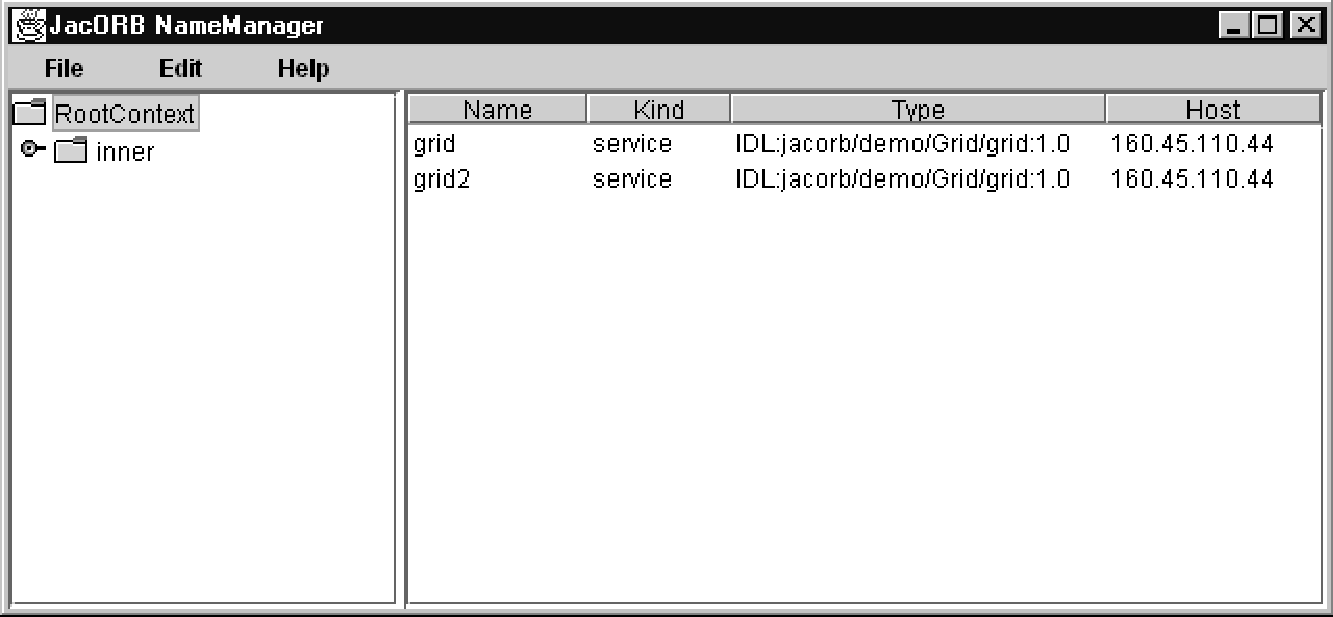
\includegraphics[width=10cm]{Naming/Nmgr1}
  \end{center}
\caption{NameManager Screenshot}
\label{fig:nameManager}
\end{figure}

NameManager has menus that let you bind and unbind names, and create
or delete naming contexts within the root context. Creating a nested
name space, e.g., can be done by selecting the {\tt RootContext} and
bringing up a context by clicking the right mouse button.  After
selecting ``new context'' from that menu, you will be prompted to
enter a name for the new, nested context.


%%% Local Variables: 
%%% mode: latex
%%% TeX-master: "../ProgrammingGuide"
%%% End: 


%%%%%%%%%%%%%%%%%%%%%%%%%%%%%%%%%%%%%%%%%%%%%%%%%%%%%%%%%%%%%%%%%%%%%%%%%%%%%%

\chapter{The server side: POA, Threads}
\label{ch:POA}


This  chapter   describes  the   facilities  offered  by   JacORB  for
controlling  how servers are  started and  executed. These  include an
activation daemon, the Portable Object Adapter (POA), and threading.

This chapter gives only a very superficial introduction to the POA.  A
thorough explanation of how the POA can be used in different settings and of
the different policies and strategies it offers is beyond our scope here, but
can be found in \cite{Brose2001a}.  Other references that explain the POA are
\cite{Henning1999, Vinoski1998}.  More in--depth treatment in C++ can be found
in the various C++-Report Columns on the POA by Doug Schmidt and Steve
Vinoski.  These articles are available at
\href{http://www.cs.wustl.edu/~schmidt/report-doc.html}{http://www.cs.wustl.edu/~schmidt/report-doc.html}.
The ultimate reference, of course, is the CORBA specification.

\section{POA}

The POA provides a comprehensive set of interfaces for managing object
references and servants. The code  written using the POA interfaces is
now portable across ORB implementations  and has the same semantics in
every ORB that is compliant to CORBA 2.2 or above.

The POA defines standard interfaces to do the following:
\begin{itemize}
\item Map an object reference to a servant that implements that object
\item Allow transparent activation of objects
\item Associate policy information with objects
\item  Make a  CORBA  object persistent  over  several server  process
lifetimes
\end{itemize}

In the POA specification, the use of pseudo-IDL has been deprecated in
favor  of an approach  that uses  ordinary IDL,  which is  mapped into
programming languages using the  standard language mappings, but which
is  locality constrained.  This means  that references  to  objects of
these types may not be passed outside of a server's address space. The
POA  interface  itself  is  one  example of  a  locality--constrained
interface.

The  object adapter  is that  part of  CORBA that  is  responsible for
creating CORBA  objects and  object references and  --- with  a little
help  from  skeletons ---  dispatching  operation  requests to  actual
object  implementations.   In  cooperation  with   the  Implementation
Repository  it can also  activate objects,  i.e. start  processes with
programs that provide implementations for CORBA objects.

\section{Threads}

JacORB  currently  offers  one   server--side  thread  model.  The  POA
responsible for a given request will obtain a request processor thread
from  a central  thread pool.  The pool  has a  certain size  which is
always between the maximum and  minimum value configure by setting the
properties     {\tt     jacorb.poa.thread\_pool\_max}     and     {\tt
jacorb.poa.thread\_pool\_min}.

When a  request arrives and  the pool is  found to contain  no threads
because all  existing threads are  active, new threads may  be started
until     the    total    number     of    threads     reaches    {\tt
jacorb.poa.thread\_pool\_max}. Otherwise,  request processing is blocked
until a  thread is returned to  the pool. Upon  returning threads that
have  finished processing a  request to  the pool,  it must  be decided
whether  the  thread  should  actually   remain  in  the  pool  or  be
destroyed. If the current pool  size is above the minimum, a processor
thread will not be out into the pool again. Thus, the pool size always
oscillates between max and min.

Setting {\tt min} to a value  greater than one means keeping a certain
number  of   threads  ready  to  service   incoming  requests  without
delay. This is  especially useful if you now  that requests are likely
to come  in in a bursty fashion.  Limiting the pool size  to a certain
maximum  is  done to  prevent  servers  from  occupying all  available
resources.

Request  processor   threads  usually   run  at  the   highest  thread
priority. It is possible to influence thread priorities by setting the
property  {\tt jacorb.poa.thread\_priority} to  a value  between Java's
Thread.MIN\_PRIORITY and Thread.MAX\_PRIORITY. If the configured priority
value  is  invalid JacORB  will  assign  maximum  priority to  request
processing threads.



%%% Local Variables: 
%%% mode: latex
%%% TeX-master: "../ProgrammingGuide"
%%% End: 


%%%%%%%%%%%%%%%%%%%%%%%%%%%%%%%%%%%%%%%%%%%%%%%%%%%%%%%%%%%%%%%%%%%%%%%%%%%%%%

\chapter{Implementation Repository}
\label{Ch_Imr}


\begin{quote}
``...  it is  very easy to be blinded to  the essential uselessness of
them by  the sense of achievement you  get from getting it  to work at
all.  In other  words --- and that is a  rock-solid principle on which
the whole of the Corporation's Galaxywide success is founded --- their
fundamental design  flaws are  completely hidden by  their superficial
design flaws.''

             D. Adams: So Long and Thanks for all the Fish
\end{quote}

The Implementation Repository is not, as its name suggests, a database
of  implementations.   Rather,  it  contains information  about  where
requests  to specific  CORBA objects  have  to be  redirected and  how
implementations  can be  transparently  instantiated if,  for a  given
request  to   an  object,  none  is   reachable.   ``Instantiating  an
implementation'' means starting a server program that hosts the target
object.  In  this  chapter  we  give  a brief  overview  and  a  short
introduction  on how to  use the  Implementation Repository.  For more
details please see \cite{Henning1999}.

\section{Overview}

Basically, the  Implementation Repository (ImR) is  an indirection for
requests  using  persistent  object  references. A  persistent  object
reference is one that was created  by a POA with a PERSISTENT lifespan
policy. This means that the lifetime of the object is longer than that
of its creating POA.   Using the Implementation Repository for objects
the lifetime  of which does not exceed  the life time of  its POA does
not make sense  as the main function of  the Implementation Repository
is to take care that such  a process exists when requests are made ---
and to start one if necessary.

To fulfill this function, the ImR  has to be involved in every request
to ``persistent  objects''.  This is achieved  by rewriting persistent
object  references to  contain {\em  not}  the address  of its  server
process but  the address  of the ImR.   Thus, requests  will initially
reach the ImR and not the actual server --- which may not exist at the
time of the request. If such a request arrives at the ImR, it looks up
the  server information  in its  internal tables  to determine  if the
target object is reachable or not.  In the latter case, the ImR has to
have  information  about how  an  appropriate  server  process can  be
started.   After   starting  this   server,  the  client   receives  a
LOCATION\_FORWARD  exception  from  the  ImR.  This  exception,  which
contains a new  object reference to the actual  server process now, is
handled by its runtime system  transparently.  As a result, the client
will automatically  reissue its request  using the new  reference, now
addressing the target directly.

\section{Using the JacORB Implementation Repository}

The  JacORB   Implementation  Repository  consists   of  two  separate
components:  a repository  process which  need  only exist  once in  a
domain, and  process startup daemons,  which must be present  on every
host that is  to start processes. Note that none  of this machinery is
necessary for processes that host  objects with a TRANSIENT life time,
such as used by the RootPOA.

First of all, the central repository process (which we will call ImR
in the following) must be started:

\cmdline{imr [-n] [-p <port>] [-i <ior\_file>][-f <file>][-b <file>] [-a]}

The   ImR   is  located   using   the   configuration  property   {\tt
ORBInitRef.ImplementationRepository}.  This property  must be set such
that  a  http  connection  can  be  made and  the  ImR's  IOR  can  be
read. Next, startup  daemons must be created on  selected hosts. To do
this, the following command must is issued on each host:

\cmdline{imr\_ssd}

When a startup  daemon is created, it contacts  the central ImR.

To register  a program such that  the ImR can start  it, the following
command is used (on any machine that can reach the ImR):

\cmdline{imr\_mg add "AServerName" -c "jaco MyServer"}

The {\tt imr\_mg} command is the  generic way of telling the ImR to do
something. It  needs another command  parameter, such as {\tt  add} in
this case. To add a server to the ImR, an {\em implementation name} is
needed. Here, it is {\tt  "AServerName"}.  If the host were the server
should be  restarted is not the  local one, use the  {\tt -h hostname}
option.  Finally, the  ImR needs to know how to  start the server. The
string {\tt "jaco  MyServer"} tells it how. The  format of this string
is simply such  that the server daemon can execute  it (using the Java
API call  {\tt exec()}), i.e.  it  must be intelligible  to the target
host's operating system.   For a Windows machine, this  could, e.g. be
{\tt "start jaco MyServer"} to have the server run in its own terminal
window, under Unix  the same can be achieved with  {\tt "xterm -e jaco
MyServer"}.

The startup  command is a  string that is  passed as the  {\em single}
argument to javas {\tt Runtime.exec()} method, without interpreting it
or adding  anything. Since {\tt  Runtime.exec()} has system--dependent
behaviour, the startup string has to reflect that. While for most unix
systems  it  is  sufficient  to  avoid shell--expansions  like  *  and
\verb+~+,  windows--based  systems  do   not  pass  the  string  to  a
commandline interpreter so a simple {\tt jaco MyServer} will fail even
if it works if directly typed in at the dos prompt. Therefore you have
to  ``wrap'' the  core  startup command  in  a call  to a  commandline
interpreter. On NT the following startup command will do the job: {\tt
cmd /c "jaco MyServer"}.  Please keep in mind that if you use the {\tt
imr\_mg} command  to set the startup  command, you have  to escape the
quotes so they appear inside of the resulting string.

If you don't  intend to have your server  automatically started by the
ImR     you      can     also     set      the     property     ``{\tt
jacorb.imr.allow\_auto\_register}'' or use the  {\tt -a} switch of the
ImR  process. If  this property  is  set, the  ImR will  automatically
create a new  entry for a server on POA activation,  if the server has
not been registered previously. In this case you don't have to use the
ImR Manager to register your server.

For a client program to be  able to issue requests, it needs an object
reference.  Up to  this  point,  we haven't  said  anything about  how
persistent object  references come into  existence. Reference creation
happens as usual, i.e. in the server application one of the respective
operations  on a  POA is  called.  For a  reference to  be created  as
``persistent'',  the POA  must  have been  created  with a  PERSISTENT
lifespan policy. This is done as in the following code snippet:

\small{
\begin{verbatim}
    /* init ORB and root POA */
    orb = org.omg.CORBA.ORB.init(args, props);
    org.omg.PortableServer.POA rootPOA =
        org.omg.PortableServer.POAHelper.narrow(
                        orb.resolve_initial_references("RootPOA"));

    /* create policies  */

    org.omg.CORBA.Policy [] policies = new org.omg.CORBA.Policy[2];
    policies[0] = rootPOA.create_id_assignment_policy(
                                IdAssignmentPolicyValue.USER_ID);
    policies[1] = rootPOA.create_lifespan_policy(
                                LifespanPolicyValue.PERSISTENT);

    /* create POA */

    POA myPOA = rootPOA.create_POA("XYZPOA",
                                rootPOA.the_POAManager(), policies);

    /* activate POAs */
    poa.the_POAManager().activate();

\end{verbatim}
}

(Note that in general the  id assignment policy will be {\tt USER\_ID}
for a POA with persistent object references because this id will often
be a key into  a database where the object state is  stored). If a POA
is created with this lifespan policy and the ORB property ``use\_imr''
is set, the ORB will try to  notify the ImR about this fact so the ImR
knows it doesn't need to start  a new process for requests that target
objects on this  POA.  To set the ORB policy,  simply set the property
{\tt  jacorb.use\_imr=on}.   The   ORB  uses  another  property,  {\tt
jacorb.implname}, as  a parameter for the  notification, i.e.~it tells
the  ImR  that a  process  using this  property's  value  as its  {\em
implementation name} is present. If  the server is registered with the
ImR, this property value has  to match the implementation name that is
used when registering.

The application  can set  these properties on  the command  line using
{\tt java -Djacorb.implname=MyName}, or in the code like this:

\small{
\begin{verbatim}
    /* create and set properties */
    java.util.Properties props = new java.util.Properties();
    props.setProperty("jacorb.use_imr","on");
    props.setProperty("jacorb.implname","MyName");

    /* init ORB  */
    orb = org.omg.CORBA.ORB.init(args, props);
\end{verbatim}
}

There are a few things  you have to consider especially when restoring
object state  at startup time or  saving the state of  your objects on
shutdown. It is important that, at startup time, object initialization
is complete when the object  is activated because from this instant on
operation calls  may come  in. The repository  knows about  the server
when the  first POA with  a PERSISTENT lifespan policy  registers, but
does not  forward object  references to clients  before the  object is
actually reachable. (Another, unreliable way to handle this problem is
to  increase the {\tt  jacorb.imr.object\_activation\_sleep} property,
so the repository waits longer for the object to become ready again.)

When the server shuts down,  it is equally important that object state
is saved by the time the last POA in the server goes down because from
this moment  the Implementation Repository regards the  server as down
and will start a new one upon requests.  Thus, a server implementor is
responsible for avoiding reader/writer problems between servers trying
to store and  restore the object state.  (One way of  doing this is to
use POA  managers to set  a POA to  holding while saving state  and to
inactive when done.)

Please keep in mind  that even if you don't have to  save the state of
your objects  on server shutdown  you {\em must} deactivate  your POAs
prior   to   exiting   your    process   (or   at   least   use   {\tt
orb.shutdown(\dots)} which  includes POA deactivation).  Otherwise the
ImR keeps the  server as active and will return  invalid IORs. In case
of  a  server crash  you  can either notify the ImR manually by  using
the  command  {\tt imr\_mg  setdown AServerName} or allow the ImR to
detect the crashed server and restart it if necessary.

\section{Server migration}

The  implementation  repository  offers  another  useful  possibility:
server migration.   Imagine the  following scenario: You  have written
your  server with  persistent  POAs,  but after  a  certain time  your
machine  seems   to  be   too  slow  to   serve  all   those  incoming
requests.  Migrating your  server to  a more  powerful machine  is the
obvious  solution.    Using  the  implementation   repository,  client
references do not contain addressing information for the slow machine,
so server migration can be done transparently to client.

Assuming  that you  added your  server to  the repository,  and  it is
running  correctly.

\cmdline{imr\_mg add AServerName -h a\_slow\_machine -c "jaco MyServer"}

The first step is to {\em  hold} the server, that means the repository
delays all requests for that server until it is released again.

\cmdline{imr\_mg hold AServerName}

Now  your server  will not  receive  any requests  for its  registered
POAs. If you can't shut your server down such that it sets itself down
at  the repository,  i.e.~your POAs  are  set to  inactive prior  to
terminating the process, you can use

\cmdline{imr\_mg setdown AServerName}

to  do  that.   Otherwise  your  POAs  can't  be  reactivated  at  the
repository because they are still logged as active.

If you  want your  server to be  restarted automatically, you  have to
tell the repository the new host and maybe a new startup command.

\cmdline{imr\_mg edit AServerName -h the\_fastest\_available\_machine\\
-c "jaco MyServer"}

If your server can be restarted automatically, you now don't even have
to start it manually, but it is instead restarted by the next incoming
request.  Otherwise start it manually on the desired machine now.

The last step is to release  the server, i.e.~let all delayed requests
continue.

\cmdline{imr\_mg release AServerName}

By now your  server should be running on  another machine, without the
clients noticing.

\section{A Note About Security}
Using the imr can pose a major security threat to your system. Imagine
the following standard setup: an imr  is running on a machine, its IOR
file is placed in a directory where  it can be read by the web server,
and several  imr\_ssds are running  on other machines. An  attacker can
now  execute processes  on the  machines the  ssds are  running  on by
taking the following steps:
\begin{enumerate}
         \item  Setting the  {\tt ORBInitRef.ImplementationRepository}
                property to the IOR file on your server.
         \item  Creating a new logical server with the desired command
           to execute as startup command on the desired host (where a
           ssd is running). This is the crucial point. The ssd calls
           {\tt Runtime.exec()} with the supplied string, and there
           is no way to check if the command does what it is supposed
           to do, i.e.~start a server.
         \item Start the server with the imr\_mg. The startup command
           of the server will be exec'd on the specified host.
\end{enumerate}

Now this should  not generally discourage you to use  the imr but show
you  that   there  are  risks,  which  can   be  reduced  significantly
nonetheless. There  are several ways  to encounter this threat  and we
don't consider this list to be complete:
\begin{enumerate}
        \item Try to control the distribution of the IOR file. Hiding
          it should not be considered here, because {\it security by
            obscurity} is generally a bad approach. Try to make use of
          file system mechanisms like groups and ACLs.
          \item Use a firewall which blocks of incoming traffic. Keep
            in mind that if the attacker is inside of your protection
            domain, the firewall won't help. It is also not that hard
            to write a Trojan that can tunnel those firewalls that
            block incoming traffic.
          \item Enforce SSL connections to the imr. This blocks all
            client connections that don't have a certificate signed by
            a CA of your choice. See chapter \ref{ch:SSL} for more
            information.
\end{enumerate}


%%% Local Variables: 
%%% mode: latex
%%% TeX-master: "../ProgrammingGuide"
%%% End: 


%%%%%%%%%%%%%%%%%%%%%%%%%%%%%%%%%%%%%%%%%%%%%%%%%%%%%%%%%%%%%%%%%%%%%%%%%%%%%%

\chapter{Dynamic Management of Any Values}
\label{ch:dynany}

{\em by Jason Courage}

The purpose of this chapter is to describe the DynAny specification,
which is the specification for the dynamic management of Any values.
This chapter only describes the main features of the DynAny
specification; for the complete specification consult the appropriate
chapter of the CORBA specification available from the OMG.

\section{Overview}

DynAny objects are used to dynamically construct and traverse Any
values.  A DynAny can represent a value of a basic type, such as
boolean or long, or a constructed type, such as enum or struct.

\section{Interfaces}

The UML diagram below shows the relationship between the interfaces
in the org.omg.DynamicAny module.

\smallskip
\begin{figure}[htb]
  \begin{center}
    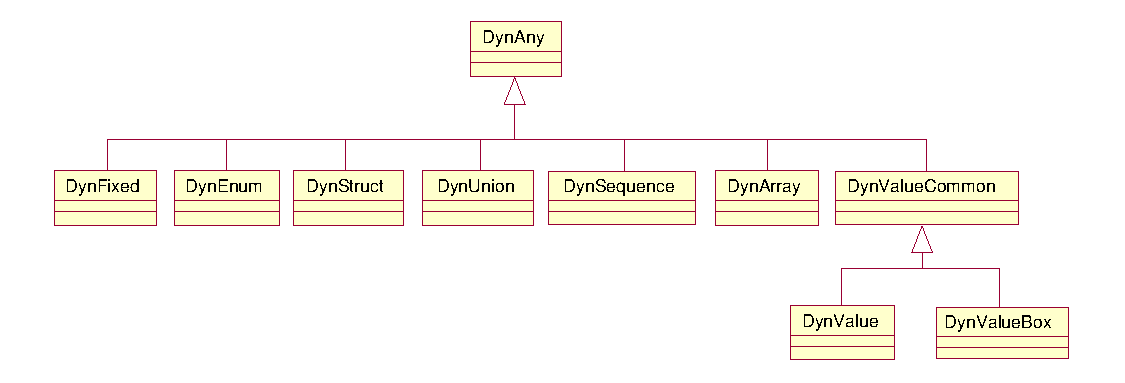
\includegraphics[width=\textwidth]{DynAny/dynany}
  \end{center}
\caption{DynAny Relationships}
\end{figure}


The DynAny interface is the base interface that represents values of
the basic types.  For each constructed type there is a corresponding
interface that extends the DynAny interface and defines operations
specific to the constructed type.  The table below lists the
interfaces in the DynamicAny module and the types they represent.


\begin{small}
\begin{longtable}{|p{6.3cm}|p{8.6cm}|}
\hline
~ \hfill \textbf {Interface} \hfill ~ & ~ \hfill \textbf {Type} \hfill ~ \endhead
\hline
\verb"DynAny" & \verb"basic types (boolean, long, etc.)" \\
\hline
\verb"DynFixed" & \verb"fixed" \\
\hline
\verb"DynEnum" & \verb"enum" \\
\hline
\verb"DynStruct" & \verb"struct" \\
\hline
\verb"DynUnion" & \verb"union" \\
\hline
\verb"DynSequence" & \verb"sequence" \\
\hline
\verb"DynArray" & \verb"array" \\
\hline
\verb"DynValue*" & \verb"non-boxed valuetype" \\
\hline
\verb"DynValueBox*" & \verb"boxed valuetype" \\
\hline

\end{longtable}
\end{small}

* Not currently implemented by JacORB.

\section{Usage Constraints}

Objects that implement interfaces in the DynamicAny module are
intended to be local to the process that constructs and uses them.
As a result, references to these objects cannot be exported to other
processes or externalized using ORB::object\_to\_string;  an
operation that attempts to do so will throw the MARSHAL system
exception.

\section{Creating a DynAny Object}

The DynAnyFactory interface is used to create a DynAny object.  There
are two operations for creating a DynAny object; these are listed in
the table below.


\begin{small}
\begin{longtable}{|p{6.3cm}|p{8.6cm}|}
\hline
~ \hfill \textbf {Operation} \hfill ~ & ~ \hfill \textbf {Description} \hfill ~ \endhead
\hline
\verb"create_dyn_any" & \verb"Constructs a DynAny object from an Any"
\verb"value" \\
\hline
\verb"create_dyn_any_from_ty"
\verb"pe_code" & \verb"Constructs a DynAny object from a"
\verb"TypeCode" \\
\hline

\end{longtable}
\end{small}

The example below illustrates how to obtain a reference to the
DynAnyFacory object and then use it to construct a DynAny object with
each of the create operations.  Exception handling is omitted for
brevity.

The following line of code imports the classes in the DynamicAny
package.

\begin{small}
\begin{verbatim}
import org.omg.DynamicAny.*;

\end{verbatim}
\end{small}

The following code segment obtains a reference to the DynAnyFacory
object.

\begin{small}
\begin{verbatim}
DynAnyFactory factory = null;
DynAny DynAny = null;
DynAny DynAny2 = null;
org.omg.CORBA.Any any = null;
org.omg.CORBA.TypeCode tc = null;
org.omg.CORBA.Object obj = null;

// obtain a reference to the DynAnyFactory
obj = orb.resolve_initial_references ("DynAnyFactory");

// narrow the reference to the correct type
factory = DynAnyFactoryHelper.narrow (obj);

\end{verbatim}
\end{small}

The following code segment creates a DynAny with each of the create
operations.

\begin{small}
\begin{verbatim}
// create a DynAny object from an Any
any = orb.create_any ();
any.insert_long (1);
DynAny = factory.create_dyn_any (any);

// create a DynAny object from a TypeCode
tc = orb.get_primitive_tc (org.omg.CORBA.TCKind.tk_long);
DynAny2 = factory.create_dyn_any_from_type_code (tc);

\end{verbatim}
\end{small}

If the Any value or TypeCode represents a constructed type then the
DynAny can be narrowed to the appropriate subtype, as illustrated
below.

The following IDL defines a struct type.

\begin{small}
\begin{verbatim}
// example struct type
struct StructType
{
   long field1;
   string field2;
};

\end{verbatim}
\end{small}

The following code segment illustrates the creation of a DynStruct
object that represents a value of type StructType.

\begin{small}
\begin{verbatim}
StructType type = null;
DynStruct dynStruct = null;

// create an Any that contains an object of type StructType
type = new StructType (999, "Hello");
any = orb.create_any ();
StructTypeHelper.insert (any, type);

// construct a DynAny from an Any and narrow it to a DynStruct
dynStruct = (DynStruct) factory.create_dyn_any (any);

\end{verbatim}
\end{small}

\section{Accessing the Value of a DynAny Object}

The DynAny interface defines a set of operations for accessing the
value of a basic type represented by a DynAny object.  The operation
to get a value of basic type $<$type$>$ from a DynAny has the form
get\_$<$type$>$.  The operation to insert a value of basic type
$<$type$>$ into a DynAny has the form insert\_$<$type$>$.  A
TypeMismatch exception is thrown if the type of the operation used to
get/insert a value into a DynAny object does not match the type of
the DynAny.

The operations for accessing the value of a constructed type
represented by a DynAny are defined in the interface specific to the
constructed type.  For example, the DynStruct interface defines the
operation get\_members, which returns a sequence of name/value pairs
representing the members of the struct or exception represented by a
DynStruct object.

\section{Traversing the Value of a DynAny Object}

DynAny objects can be viewed as an ordered collection of component
DynAnys.  For example, in a DynStruct object the ordered collection
of component DynAnys is the members of the struct or exception it
represents.  For DynAny objects representing basic types or
constructed types that do not have components, the collection of
component DynAnys is empty.

All DynAny objects have a current position.  For DynAnys representing
constructed types that have components, the current position is the
index of the component DynAny that would be obtained by a call to the
current\_component operation (described in the table below).  The
component DynAnys of a DynAny object are indexed from 0 to n-1, where
n is the number of components.  For DynAnys representing basic types,
or constructed types that do not have components, the current
position is fixed at the value -1.

The operations for traversing the component DynAnys of a DynAny
object are common to all DynAny subtypes, hence they are defined in
the DynAny base interface.  The table below lists the operations
available for traversing a DynAny object.


\begin{small}
\begin{longtable}{|p{6.3cm}|p{8.6cm}|}
\hline
~ \hfill \textbf {Operation} \hfill ~ & ~ \hfill \textbf {Description} \hfill ~ \endhead
\hline
\verb"seek" & \verb"Sets the current position to the"
\verb"specified index" \\
\hline
\verb"rewind" & \verb"Sets the current position to the first"
\verb"component (index 0)" \\
\hline
\verb"next" & \verb"Advances the current position to the"
\verb"next component" \\
\hline
\verb"component_count" & \verb"Returns the number of components" \\
\hline
\verb"current_component" & \verb"Returns the component at the current"
\verb"position" \\
\hline

\end{longtable}
\end{small}

The following code segment illustrates one way of traversing the
component DynAnys of a DynStruct object.  As the DynStruct is
traversed, the value of each component is obtained and printed.
Exception handling is omitted for brevity.

\begin{small}
\begin{verbatim}
DynAny curComp = null;

// print the value of the first component
curComp = dynStruct.current_component ();
System.out.println ("field1 = " + curComp.get_long ());

// advance to the next component
dynStruct.next ();

// print the value of the second component
curComp = dynStruct.current_component ();
System.out.println ("field2 = " + curComp.get_string ());

\end{verbatim}
\end{small}

The next code segment illustrates another way to perform the same
task.

\begin{small}
\begin{verbatim}
// go back to the first component
dynStruct.rewind ();  // same as calling seek (0)

// print the value of the first component
System.out.println ("field1 = " + dynStruct.get_long ());

// advance to the next component
dynStruct.seek (1);

// print the value of the second component
System.out.println ("field2 = " + dynStruct.get_string ());

\end{verbatim}
\end{small}

As the second code segment illustrates, if the component DynAny
represents a basic type, its value can be extracted (or inserted) by
calling the accessor operation on the parent DynAny directly, rather
than first obtaining the component using the current\_component
operation.

\section{Constructed Types}

This section describes the interfaces in the DynamicAny module that
represent the constructed types supported by JacORB.  Each of these
interfaces extends the DynAny interface.



\subsection{DynFixed}

A DynFixed object represents a fixed value.  Since IDL does not have
a generic type to represent a fixed type, the operations in this
interface use the IDL string type.  The value represented by a
DynFixed object can be accessed (as a string) using the get\_value
and set\_value operations.

A DynFixed object has no components.

\subsection{DynEnum}

A DynEnum object represents a single enumerated value.  The integer
(ordinal) value of the enumerated value can be accessed with the
get\_as\_ulong and set\_as\_ulong operations.  The string (IDL
identifier) value of the enumerated value can be accessed with the
get\_as\_string and set\_as\_string operations.

A DynEnum object has no components.

\subsection{DynStruct}

A DynStruct object represents a struct value or an exception value.
The current\_member\_name and current\_member\_kind operations return
the name and TCKind value of the TypeCode of the member at the
current position of the DynStruct.  The members of the DynStruct can
be accessed with the get\_members and set\_members operations.

The component DynAnys of a DynStruct object are the members of the
struct or exception.  A DynStruct representing an empty exception has
no components.

\subsection{DynUnion}

A DynUnion object represents a union value.  The value of the
discriminator can be accessed using the get\_discriminator and
set\_discriminator operations.

If the discriminator is set to a value that names a member of the
union then that member becomes active.  Otherwise, if the value of
the discriminator does not name a member of the union then there is
no active member.

If there is an active member, the member operation returns its value
as a DynAny object, and the member\_name and member\_kind operations
return its name and the TCKind value of its TypeCode.  These
operations throw an InvalidValue exception if the union has no active
member.

A DynUnion object can have either one or two components.  The first
component is always the discriminator value.  The second component is
the value of the active member, if one exists.

\subsection{DynSequence}

A DynSequence object represents a sequence.  The length of the
sequence can be accessed using the get\_length and set\_length
operations.  The elements of the sequence can be accessed using the
get\_elements and set\_elements operations.

The component DynAnys of a DynSequence object are the elements of the
sequence.

\subsection{DynArray}

A DynArray object represents an array.  The elements of the array can
be accessed using the get\_elements and set\_elements operations.

The component DynAnys of a DynArray object are the elements of the
array.

\section{Converting between Any and DynAny Objects}

The DynAny interface defines operations for converting between Any
objects and DynAny objects.  The from\_any operation initialises the
value of a DynAny with the value of a specified Any.  A TypeMismatch
exception is thrown if the type of the Any does not match the type of
the DynAny.  The to\_any operation creates an Any from a DynAny.

As an example of how these operations might be useful, suppose one
wants to dynamically modify the contents of some constructed type,
such as a struct, which is represented as an Any.  The following
steps will accomplish this task:

\begin{enumerate}
  \item  A DynStruct object is constructed from the TypeCode of the struct using the DynAnyFactory::create\_dyn\_any\_from\_type\_code operation.
  \item  The DynAny::from\_any operation is used to initialise the value of the DynStruct with the value of the Any.
  \item  The contents of the DynStruct can now be traversed and modified.
  \item  A new Any can be created to represent the modified struct using the DynAny::to\_any operation.
\end{enumerate}

\section{Further Examples}

The demo/dynany directory of the JacORB repository contains example
code illustrating the use of DynAny objects.  Further code can be
found in the org.jacorb.test.orb.dynany package of the JacORB-Test
repository.


%%% Local Variables: 
%%% mode: latex
%%% TeX-master: "../ProgrammingGuide"
%%% End: 


%%%%%%%%%%%%%%%%%%%%%%%%%%%%%%%%%%%%%%%%%%%%%%%%%%%%%%%%%%%%%%%%%%%%%%%%%%%%%%
\chapter{Objects By Value}
\label{ch:obv}


Until CORBA 2.3, objects could only be passed using reference
semantics: there was no way to specify that object state should be
copied along with an object reference. A further restriction of the
earlier CORBA versions was that all non-object types (structs, unions,
sequences, etc.) were {\em values}, so you could not use, e.g. a
reference-to-struct to construct a graph of structure values that
contained shared nodes. Finally, there was no inheritance between
structs.

All these shortcomings are addressed by the {\em objects-by-value} (OBV)
chapters of the CORBA specification: the addition of stateful
value types supports copy semantics for objects and inheritance for
structs, boxed value types introduce reference semantics for base
types, and abstract interfaces determine whether an argument is sent
by-value or by-reference by the argument's runtime type. The
introduction of OBV into CORBA presented a major shift in the CORBA
philosophy, which had been to strictly avoid any dependence on
implementation details (state, in particular). It also added a
considerable amount of marshaling complexity and interoperability
problems. (As a personal note: Even in CORBA 2.6, the OBV marshaling
sections are still not particularly precise...)

JacORB 2.0 implements most of the OBV specification.  Boxed value
types and regular value types work as prescribed in the standard
(including value type inheritance, recursive value types, and
factories).  Still missing in the current implementation is run-time
support for abstract value types (although the compiler does accept
the corresponding IDL syntax), and the marshaling of truncatable
value types does not yet meet all the standard's requirements (and
should thus be called ``beta'').

\section{Example}

To illustrate the use of various kinds of value types, here's an
example which is also part of the demo programs in the JacORB
distribution.  The demo shows the use of boxed value types and a
recursive stateful value type. Here's the IDL definition from {\tt
demo/value/server.idl}:

\begin{verbatim}
module demo {
  module value {

     valuetype boxedLong   long;
     valuetype boxedString string;

     valuetype Node {
        public long id;
        public Node next;
     };

     interface ValueServer {
        string receive_long   (in boxedLong p1, in boxedLong p2);
        string receive_string (in boxedString s1, in boxedString s2);
        string receive_list   (in Node node);
     };
  };
};
\end{verbatim}

From the definition of the  boxed value type {\tt boxedLong} and
{\tt boxedString}, the IDL generates the following Java class, which
is simply a holder for the long value. No mapped class is generated
for the boxed string value type.

\begin{verbatim}
package demo.value;

public class boxedLong
    implements org.omg.CORBA.portable.ValueBase
{
    public int value;
    private static String[] _ids = { boxedLongHelper.id() };

    public boxedLong(int initial )
    {
        value = initial;
    }
    public String[] _truncatable_ids()
    {
        return _ids;
    }
}
\end{verbatim}

The boxed value definitions in IDL above permit uses of non-object
types that are not possible with IDL primitive types. In particular, it
is possible to pass Java {\tt null} references where a value of a
boxed value type is expected. For example, we can call the operation
{\tt receive\_long} and pass one initialized {\tt boxedLong} value and
a null reference, as show in the following snippet from the client
code:

\begin{verbatim}
    ValueServer s = ValueServerHelper.narrow( obj );
    boxedLong boxL = new boxedLong (774);

    System.out.println ("Passing two integers: "
                       + s.receive_long ( boxL , null ));
\end{verbatim}

With a regular {\tt long} parameter, a {\tt null} reference would have
resulted in a {\tt BAD\_PARAM} exception. With boxed value types, this
usage is entirely legal and the result string returned from the {\tt
  ValueServer} object is {\tt ``one or two null values''}.

A second new possibility of the reference semantics that can be
achieved by ``boxing'' primitive IDL types is {\em sharing} of values.
With primitive values, two variables can have copies of the same
value, but they cannot both refer to the same value. This means that
when one of the variables is changed, the other one retains its
orignal value. With shared values that are {\em referenced}, both
variables would always point to the same value.

The stateful value type {\tt Node} is implemented by the programmer in
a class {\tt NodeImpl} (see the JacORB distribution for the actual
code).  The relationship between this implementation class and the
corresponding IDL definition is not entirely trivial, and we will
discuss it in detail below.

\section{Factories}

When an instance of a (regular) value type is marshaled over the wire
and arrives at a server, a class that implements this value type must
be found, so that a Java object can be created to hold the state
information.  For interface types, which are only passed by
reference, something similar is accomplished by the POA, which
accepts remote calls to the interface and delivers them to a local
implementation class (the \emph{servant}).  For value type instances,
there is no such thing as a POA, because they cannot be called
remotely.  Thus, the ORB needs a different mechanism to know which
Java implementation class corresponds to a given IDL value type.

The CORBA standard introduces \emph{value factories} to achieve this.
Getting your value factories right can be anywhere from trivial to
tricky (we will cover the details in a minute), and so the standard
suggests that ORBs also provide convenience mechanisms to relieve
programmers from writing value factories if possible.  JacORB's
convenience mechanism is straightforward:

\begin{quotation}
\noindent \emph{If the implementation class for an IDL value type A is named
  AImpl, resides in the same package as A, and has a no-argument
constructor, then no value factory is needed for that type.}
\end{quotation}

In other words, if your implementation class follows the common naming
convention (``...Impl''), and it provides a no-arg constructor
so that the ORB can instantiate it, then the ORB has all that it
needs to (a) find the implementation class, and (b) create an instance
of it (which is then initialized with the unmarshaled state from the
wire).

This mechanism ought to save you from having to write a value factory
99\% of the time.  It works for all kinds of regular value types,
including those with inheritance, and recursive types (where a type
has members of its own type).

If you do need more control over the instance creation process, or the
unmarshaling from the wire, you can write your own value factory
class and register it with the ORB using {\tt
ORB.register\_value\_factory(}\emph{repository\_id, factory}{\tt)}.
The \emph{factory} object needs to implement the interface {\tt
org.omg.CORBA.portable.ValueFactory}, which requires a single method:

\begin{verbatim}
   public Serializable read_value (InputStream is);
\end{verbatim}

When an instance of type \emph{repository\_id} arrives over the wire,
the ORB calls the {\tt read\_value()} method, which must unmarshal the
data from the input stream, create an instance of the appropriate
implementation class from it, and return that.

The easiest way to implement this method is to create an instance of
the implementation class, and pass it to the {\tt read\_value()} method
of the given InputStream:

\begin{verbatim}
   public Serializable read_value (InputStream is) {
     A result = new AImpl();
     return is.read_value(result);
   }
\end{verbatim}

The {\tt InputStream.read\_value()} method registers the newly created
instance in the stream's indirection table, and then reads the data
from the stream and initializes the given {\tt value} instance from
it.

The value factory must be registered with the ORB using {\tt
 register\_value\_factory()}.  As a special convenience (defined in
 the CORBA standard), if the value factory class for type {\tt A} is
 called {\tt ADefaultFactory}, then the ORB will find it automatically
 and use it, unless a different factory has been explicitly
 registered.

It sometimes causes confusion that you can also define \emph{factory
methods} in a value type's IDL.  These factory methods are completely
unrelated to the unmarshaling mechanism discussed above; they are
simply a portable means to declare what kinds of ``constructors'' a
value type implementation should have.  They are purely for local use,
but since they are ``factories'', the corresponding methods must also
be implemented in the type's {\tt ValueFactory} implementation.


%%% Local Variables: 
%%% mode: latex
%%% TeX-master: "../ProgrammingGuide"
%%% End: 


%%%%%%%%%%%%%%%%%%%%%%%%%%%%%%%%%%%%%%%%%%%%%%%%%%%%%%%%%%%%%%%%%%%%%%%%%%%%%%
\chapter{Interface Repository}
\label{ch:interface_repository}

%
% IFR
% $Id: ifr.tex,v 1.2 2006-05-15 13:19:58 alphonse.bendt Exp $
% 

Run--time  type information  in CORBA  is  managed by  the ORB's  {\it
Interface Repository}  (IR) component.  It allows  to request, inspect
and modify IDL  type information dynamically, e.g., to  find out which
operations an object supports. Some ORBs  may also need the IR to find
out whether  a given object's type  is a subtype of  another, but most
ORBs can do  without the IR by encoding this  kind of type information
in the helper classes generated by the IDL compiler.

In essence,  the IR is  just another remotely accessible  CORBA object
that offers  operations to retrieve  (and in theory also  modify) type
information.

\section{Type Information in the IR}

The  IR  manages  type   information  in  a  hierarchical  containment
structure that  corresponds to the structure of  scoping constructs in
IDL  specifications:   modules  contain  definitions   of  interfaces,
structures, constants  etc. Interfaces in turn  contain definitions of
exceptions, operations, attributes  and constants. Figure \ref{IR-fig}
illustrates this hierarchy.

\begin{figure}[htb]
  \begin{center}
    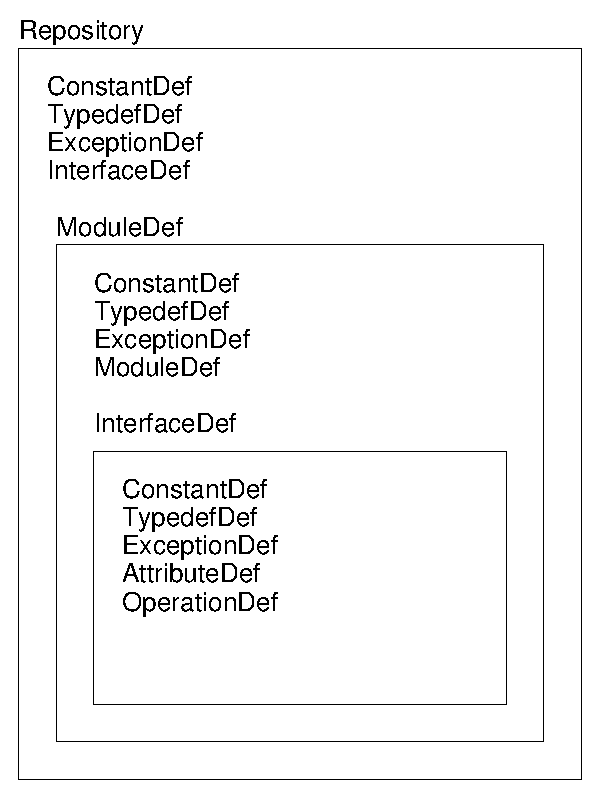
\includegraphics[width=5cm]{IFR/IR}
  \end{center}
\caption{Containers in the Interface Repository}
\label{IR-fig}
\end{figure}

The  descriptions  inside  the  IR  can  be  identified  in  different
ways. Every  element of  the repository has  a unique,  qualified name
which  corresponds  to  the  structure  of  name  scopes  in  the  IDL
specification. An interface {\tt  I1} which was declared inside module
{\tt M2} which in turn was  declared inside module {\tt M1} thus has a
qualified name  {\tt M1::M2::I1}. The  IR also provides  another, much
more   flexible   way   of    naming   IDL   constructs   using   {\it
Repository Id}s.  There   are  a   number  of  different   formats  for
RepositoryIds  but  every  Repository  must  be  able  to  handle  the
following format, which is marked  by the prefix {\tt "IDL:"} and also
carries  a  suffix   with  a  version  number,  as   in,  e.g.,  "{\tt
IDL:jacorb/demo/grid:1.0}". The name  component between the colons can
be set freely using the  IDL compiler directives {\tt \#pragma prefix}
and {\tt \#pragma ID}. If no such directive is used, it corresponds to
the qualified name as above.

\section{Repository Design}

When designing the  Interface Repository, our goal was  to exploit the
Java reflection  API's functionality to  avoid having to  implement an
additional data base for  IDL type descriptions. An alternative design
is to use the IR as a back-end to the IDL compiler, but we did not want
to  introduce such  a  dependency and  preferred  to a  have a  rather
``light--weight'' repository  server.  As  it turned out,  this design
was  possible because  the similarities  between the  Java  and CORBA
object models allow  us to derive the required  IDL information at run
time. As  a consequence,  we can  even do without  any IDL  at compile
time.  In addition  to this simplification, the main  advantage of our
approach lies in avoiding  redundant data and possible inconsistencies
between  persistent IDL descriptions  and their  Java representations,
because Java classes have to be generated and stored anyway.

Thus, the  Repository has to  load Java classes, interpret  them using
reflection  and   translate  them   into  the  appropriate   IDL  meta
information. To  this end, the  repository realizes a  reverse mapping
from   Java   to  IDL.   Figure   \ref{IR-Process}  illustrates   this
functionality,  where $f^{-1}$  denotes  the reverse  mapping, or  the
inverse of  the language  mapping.

\begin{figure}[htb]
  \begin{center}
    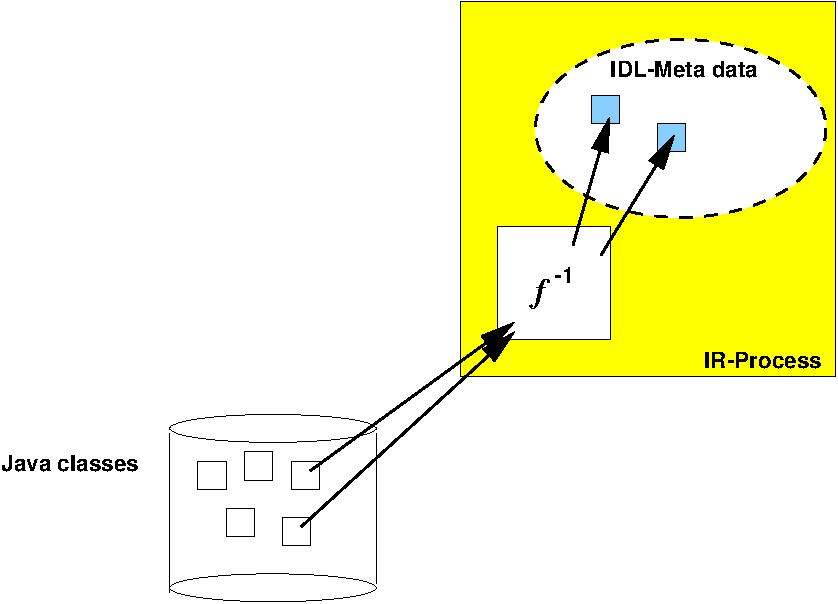
\includegraphics[width=7cm]{IFR/IR-Process}
\end{center}
\caption{The JacORB Interface Repository}
\label{IR-Process}
\end{figure}

\section{Using the IR}

For the ORB to be able to contact the IR, the IR server process must
be running. To start it, simply type the {\tt ir} command and provide
the required arguments:

\cmdline{ir /home/brose/classes /home/brose/public\_html/IR\_Ref}

The first  argument is  a path to  a directory containing  {\tt .class}
files and packages. The IR  loads these classes and tries to interpret
them as  IDL compiler--generated classes.  If it  succeeds, it creates
internal representations  of the  adequate IDL constructs. See below for
instructions on generating classes with IR information. The second
argument on  the command  line above  is simply the  name of  the file
where the IR stores its object reference for ORB bootstrapping.

To view the contents of the repository, you can use the GUI IRBrowser
tool or the query command. First, let's query the IR for a particular
repository ID. JacORB provides the command {\tt qir} (``query IR'')
for this purpose:

\cmdline{qir IDL:raccoon/test/cyberchair/Paper:1.0}

As result, the IR returns an InterfaceDef object, and {\tt qir} parses
this and prints out:

\begin{verbatim}
     interface Paper
     {
        void read(out string arg_0);
        raccoon::test::cyberchair::Review getReview(in long arg_0);
        raccoon::test::cyberchair::Review submitReview(
            in string arg_0, in long a rg_1);
        void listReviews(out string arg_0);
     };
\end{verbatim}

To start the IRBrowser, simply type

\cmdline{irbrowser [ -i <IOR-string> | -f <filename>]}

e.g.

\cmdline{irbrowser}

Note that if no arguments are supplied it will default to using
resolve\_initial\_references.

Figure \ref{fig:IRBrowser} gives a screen shot of the IR browser.

\bigskip
\begin{figure}[htb]
  \begin{center}
    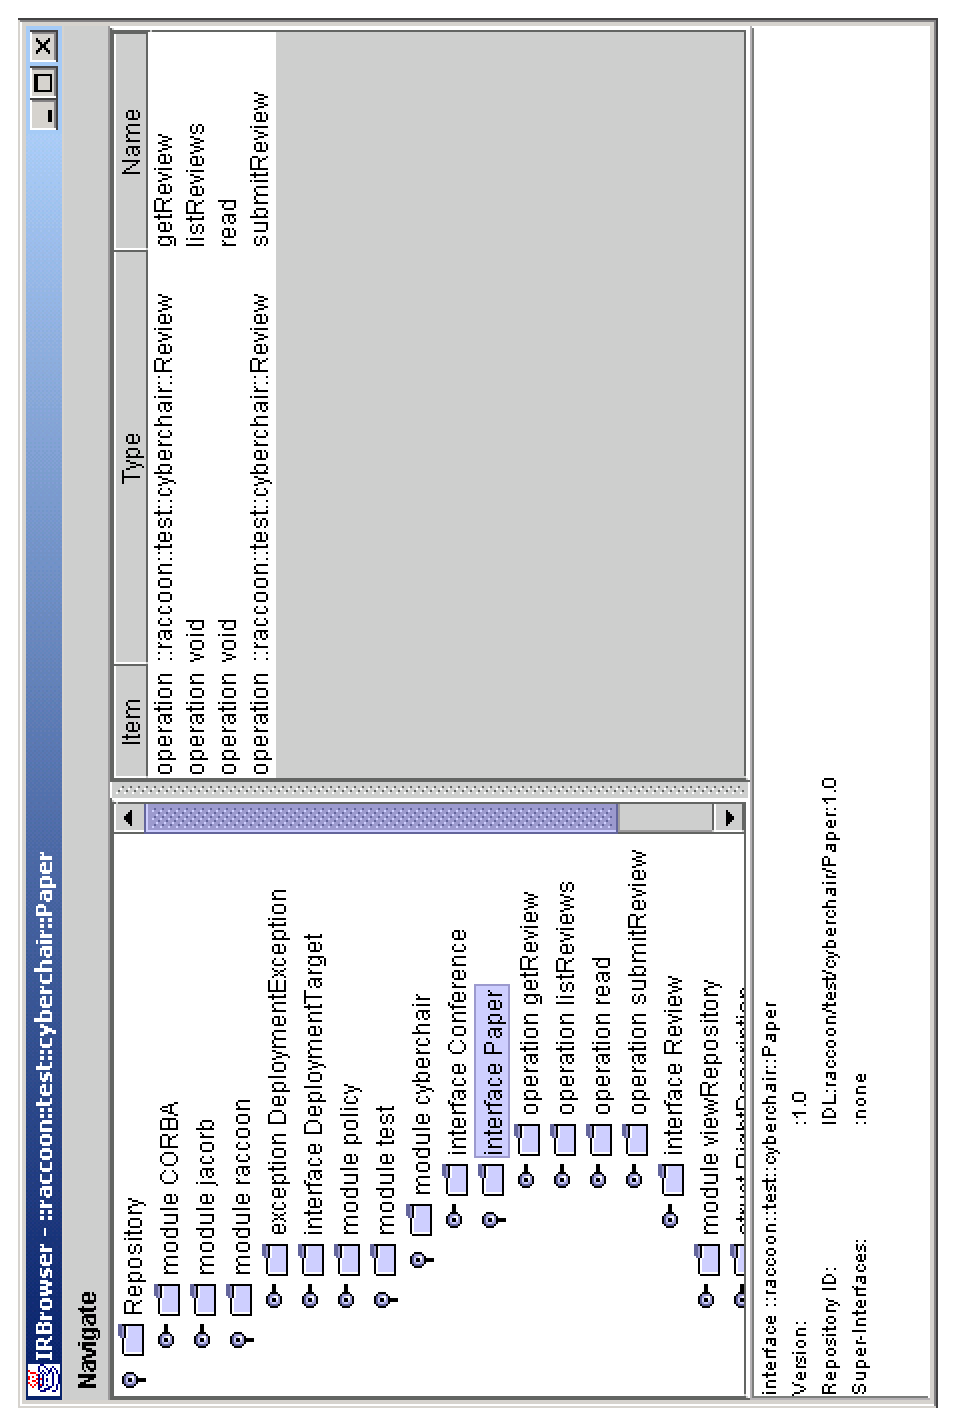
\includegraphics[width=11cm]{IFR/IRBrowser}
\end{center}
\caption{IRBrowser Screenshot}
\label{fig:IRBrowser}
\end{figure}

The Java classes generated by  the IDL compiler using the standard OMG
IDL/Java language mapping do not contain enough information to rebuild
all  of the  information contained  in  the original  IDL file.   For
example,  determining whether an  attribute in  an interface  was {\tt
readonly} or  not is not  possible, or telling the  difference between
{\tt  in}  and {\tt  inout}  parameter  passing  modes. Moreover,  IDL
modules are not  explicitly represented in Java, so  telling whether a
directory in  the class  path represents an  IDL module is  not easily
possible. For these  reasons, the JacORB IDL compiler  generates a few
additional  classes that hold  the required  extra information  if the
compiler switch {\tt -ir} is used when compiling IDL files:

\cmdline{idl -ir myIdlFile.idl}

The additional files generated by the compiler are:
\begin{itemize}
\item a {\tt \_XModule.java} class file for any IDL module X
\item a {\tt YIRHelper.java} class file for any interface Y.
\end{itemize}

\textbf{If no {\tt .class} files that  are compiled from  these extra
classes are found  in the class path passed  to the IR server  process,
the IR will not  be able  to derive any  representations.}
Note that  the IDL compiler does not make any non--compliant modifications
to any of the standard files that are defined in the Java language mapping
 --- there is only additional information.

One more caveat about these  extra classes: The compiler generates the
{\tt  \_XModule.java} class  only  for genuine  modules. Java  package
scopes created by applying the {\tt -d } switch to the IDL compiler do
not  represent   proper  modules  and   thus  do  not   generate  this
class. Thus, the contents of  these directories will not be considered
by the IR.

When an  object's client  calls the {\tt  get\_interface()} operation,
the ORB consults the IR  and returns an {\tt InterfaceDef} object that
describes the object's  interface. Using {\tt InterfaceDef} operations
on  this  description  object,  further  description  objects  can  be
obtained,  such as descriptions  for operations  or attributes  of the
interface under consideration.

The IR  can also be  called like any  other CORBA object  and provides
{\tt lookup()}  or {\tt lookup\_name()} operations to  clients so that
definitions can be searched for, given a qualified name. Moreover, the
complete contents of individual containers (modules or interfaces) can
be listed.

Interface   Repository  meta   objects  provide   further  description
operations. For a given {\tt  InterfaceDef} object, we can inspect the
different  meta   objects  contained   in  this  object   (e.g.,  {\tt
OperationDef} objects). It is  also possible to obtain descriptions in
form of a simple structure  of type {\tt InterfaceDescription} or {\tt
FullInterfaceDescription}. Since structures are  passed by value and a
{\tt   FullInterfaceDescription}    fully   provides   all   contained
descriptions,  no  further  ---possibly  remote  ---  invocations  are
necessary for searching the structure.


%%% Local Variables: 
%%% mode: latex
%%% TeX-master: "../ProgrammingGuide"
%%% End: 


%%%%%%%%%%%%%%%%%%%%%%%%%%%%%%%%%%%%%%%%%%%%%%%%%%%%%%%%%%%%%%%%%%%%%%%%%%%%%%
\chapter{The JacORB Appligator}
\label{ch:applets}


{\em by Sebastian M{\"u}ller and Steve Osselton}

\bigskip

Version 1.4 of JacORB includes a new implementation of the Appligator.
This is a portable interceptor based IIOP proxy.  Using this proxy you
can both run Java Applets with JacORB and use JacORB across firewalls
and the Internet. This new implementation no longer supports HTTP
tunneling.

\section{Appligator Functionality}

The Appligator is a GIOP proxy. When the Appligator is used, instead
of a client calling directly to a server it calls to the Appligator
which then itself calls on to the server. This is all transparent as
far as a client is concerned.  The basic mechanism of operation is as
follows:

\begin{enumerate}
\item A client that wishes to use the Appligator installs a client
  side interceptor.
\item When the client makes a call the interceptor checks to determine
  whether the call should be redirected to an Appligator. If so, then
  the original call target is encoded within a service context and a
  ForwardRequest exception is thrown so that the ORB redirects the
  call to the Appligator.
\item When the Appligator receives a forwarded request it extracts the
  original target from the service context and calls onto the original
  target. The actual proxy implementation within the Appligator is
  invoked via DSI and calls on to the target via DII.
\end{enumerate}

\section{Using The Appligator}

The Appligator can be run as a normal CORBA server via the
'appligator' shell script or batch file. The Appligator is configured
vis both command line arguments and properties stored in the ORB
configuration file 'jacorb.properties'.

\subsection{Starting Appligator}

The Appligator can be invoked as follows:

\verb+$ appligator <port> <filename> [-dynamic]+

This starts the Appligator on the specified port and writes it's IOR
to the specified file.

The '-dynamic' flag is optional and determines whether the object key
used for the Appligator IOR is dynamically (i.e. randomly) selected or
fixed. If a fixed id is used then the configuration property
'jacorb.ProxyServer.ID' is used as the object key value. If this is
not set then this defaults to 'Appligator'. Using a fixed object key
has the advantage that this key is used every time the Appligator
restarts so a remote client would not have to update it's reference to
the Appligator (typically an IOR file).

\subsection{Client Configuration}

Appligator clients need to install the appropriate client side
interceptor class. This can be done by configuring the portable ORB
initializer class 'ProxyClientInitializer' by setting the following
ORB initialization property:

{\noindent\tt\small
  org.omg.PortableInterceptor.ORBInitializerClass.org.jacorb.\\
proxy.ProxyClientInitializer}

\subsection{Appligator Configuration Appligator}

configuration properties are
placed in the 'jacorb.properties' file, all have the common prefix
'jacorb.ProxyServer'. Configuration properties are used either for the
configuration of the Appligator server itself or for the configuration
of Appligator clients.

\subsubsection{Appligator Server Properties}

If the 'jacorb.ProxyServer.Name' property is set and the name service
has been configured and is available then the Appligator will register
itself in the name service using this name.  If the
'jacorb.ProxyServer.ID' property is set and the Appligator has not
been run with the '-dynamic' flag then this property is used as the
object key in the created Appligator IOR.

\subsubsection{Appligator Client Properties}

The 'jacorb.ProxyServer.URL' configuration property is used
by clients to locate the default Appligator. This URL should map to an
IOR file written by an Appligator.  If the
'jacorb.ProxyServer.Network' and 'jacorb.ProxyServer.Netmask'
properties are set these are used to determine the local network
address for a client. If this is set then any calls to objects within
this network will not be redirected to the Appligator. This is useful
when a CORBA server may need to call to an Appligator to access remote
servers but may want to communicate with local servers directly. The
dotted decimal form should be used for both these properties, for
example:

\verb+jacorb.ProxyServer.Netmask=255.255.255.0+

\verb+jacorb.ProxyServer.Network=160.45.110.0+

Clients can be configured to use different Appligators to access
objects in different subnets. To do this configuration properties of
the form 'jacorb.ProxyServer.URL-<network>-<netmask>' can be
used. Here the URL property should map to the Appligator IOR for the
particular subnet identified by <network> and <netmask>. For example:

\verb+jacorb.ProxyServer.URL-160.45.120.0-255.255.255.0=file:/tmp/net1.ior+

\section{Applet Support}

Regular Java programs can connect to every host on the Internet,
applets can only open connections to their applethost (the host they
are downloaded from). This lets Applets only use CORBA servers on
their applethost, if no proxy is used. With JacORB Appligator, access
for your Applets is no longer restricted. Placed on the applethost,
Appligator handles all connections from and to your Applet
transparently.

Due to the transparency of JacORB Appligator you can write your Applet
as if it were a normal CORBA program. The only thing you have to do is
to use a special initialization of the ORB by calling the ORB init
operation that takes an Applet as a parameter:

\verb+ORB orb = ORB.init (applet, properties);+

A normal JacORB program reads a local jacorb.properties file to get
the URL of its name server and other vital settings. An Applet of
course has no local properties file, but a remote one: You have to
place the properties file (which has the same syntax and parameters as
the normal file) in the same directory as your Applet (the file name
has to be: jacorb.properties, without a leading dot).

Similar to the name server, Appligator writes its IOR to a file. Your
Applet has to know the location of this file to retrieve the IOR of
Appligator. You must set the location of the IOR file via the
jacorb.properties file (jacorb.ProxyServer.URL) or with an Applet
parameter in the <APPLET> HTML tag (JacorbProxyServerURL).

\subsection{Summary}

\begin{itemize}
\item Init the ORB with jacorb.orb.init(applet,properties), where applet is
this Applet and properties are java.util.Properties (which can be
null).
\item Put a jacorb.properties file in the directory of the Applet.
\item Specify the location for the Appligator IOR file in the
jacorb.properties (jacorb.ProxyServer.URL) or in an Applet parameter
(JacorbProxyServerURL)
\item Make sure the name server IOR file is
accessible for the Applet (lies on the applethost)
\item Start Appligator on the applethost (web server) with:

\verb+$ appligator <port> <filename>+

Where filename is the location where the Appligator IOR is written and is the location specified in the JacORB properties file or Applet parameter.
\end{itemize}

\subsection{Applet Properties}

As described above there are some ways for the Applet to get its JacORB properties file. The most important property is the URL to the Appligator IOR file. Without this property the Applet will not work. If you use a name server, the URL to the name server IOR must also be specified.

Properties can be set in three ways:
\begin{enumerate}
\item In the ORB.init() call with the java.util.Properties parameter.
\item In the JacORB properties file located in the same directory as
  the Applet
\item The URL to the name server and Appligator IOR file can be set in
  the Applet tag in the HTML file
\end{enumerate}


\subsection{Appligator and Netscape/IE, appletviewer}

Netscape Navigator/Communicator comes with its own (outdated) CORBA
support. You have to delete Netscape's CORBA classes to use JacORB. To
do this you have to delete the file iiop10.jar located in NS
ROOT/java/classes. It's a good idea to store a backup of Netscape's
file in another directory. Note that renaming this jar file in the
original directory does not suffice if you don't also change the .jar
extension because Netscape loads all jar files in this directory. You
then need to install jacorb.jar in this directory.

If Netscape loads wrong classes or throws security exceptions (have a
look at Netscape's Java Console to see this) be sure to check your
CLASSPATH and look for old jar files or ``.''. Remove all JacORB and
VisiBroker classes from your CLASSPATH. We succeeded running JacORB
Applet clients on Netscape  4.72 with the Java 1.3 plugin.

Microsoft's Internet Explorer is stricter than Netscape: Even
downloaded classes are not allowed to listen on a socket. We strongly
advise to use Sun's Java 1.3 plugin with IE also. To trick IE into
using JacORB, you need to copy JacORB classes to
\$WINNT$\backslash$Java$\backslash$TrustLib. You can either copy the
entire jacorb.jar and unpack it in this directory or just copy the
directories jacorb, org,and HTTPClient.

Appligator works well with Sun's appletviewer. You only have to make
the appletviewer replace the Sun's CORBA classes with JacORB's
classes. A typical appletviewer call for JacORB Applets looks like
this (written in one command line):

\verb+$ appletviewer http://www.example.com/CORBA/dii example.html+

There is a shell script called ''jacapplet'' in JacORB's bin
directory, which calls the appletviewer with the appropriate options
(you have to edit it to match your local JDK path).

If you use the Appligator with other browsers or if you know a way to
load the JacORB classes without removing and copying jars please let
us know.

\subsection{Examples}

There are some example applets in the demo directory
(jacorb/demo/applet). They are based on the normal examples. The
examples include a HTML file which calls the Applet. To run the
example start the name server first. Start Appligator on your web
server and than the normal example server corresponding to the Applet
example on any computer in any order. Then you can call the example
Applet with the JDK appletviewer or Netscape.

Be sure to have a jacorb.properties file and the jacorb.jar in place.

\section{Firewall Support}

Typically firewalls do two things: filter traffic by port, and filter
traffic by protocol. The JacORB Appligator can be used to deal with
port restrictions.

The Appligator was written to avoid the sandbox restrictions for Java
applets. Unsigned applets can only have connections to the host they
are loaded from, which makes them useless in most distributed CORBA
scenarios. The Appligator is a GIOP proxy, which enables applets to
connect to every CORBA server by redirecting the traffic from the
Applet to the CORBA server to the proxy. The Appligator also works the
other way round: Every connection the Applet is redirected to the
Appligator.

Even without applets the Appligator can be used as a GIOP proxy on a
firewall. The Appligator is a CORBA object itself and is explicitly
started on a given port using a command line argument <port>. All
incoming traffic to the Appligator will go to port <port>. If you
configure your CORBA object behind the firewall to be aware of the
Appligator all traffic from and to this objects will go through the
Appligator.

To make your port filtering firewall working with CORBA and GIOP
messages you must ask your system administrator to assign a port for
GIOP messages on the firewall. Start the Appligator on this port.

Now all CORBA servers (which are aware of the Appligator) in your
enclave can be contacted over the Appligator. If your CORBA client
wants to contact a server in the Internet outside the firewall the
connection will go over the Appligator. Callbacks from the Internet to
your client do not work with Netscape.

Finally you have to specify the location on the Appligator. This is
done the same way as JacORB determines to location of the name server:
When the Appligator starts the IOR of the Appligator is written to a
file which is put to the location you specified as command
parameter. This file must be accessible to all clients that want to
use the Appligator. You can use a shared file system to access this
file or put it on a web server etc. The location of the file in which
the IOR of the Appligator is stored must be set in the
jacorb.properties file. Use the ''jacorb.ProxyServer.URL'' property
for this.

\subsection{Summary}

\begin{itemize}
\item Use the Appligator as a GIOP proxy on a firewall if your
  firewall is configured to block all traffic but traffic on some
  special ports.
\item Ask your system administrator to assign a special port for GIOP
  on your firewall and start the Appligator on this port on the
  firewall: for example:
\verb+$ appligator 7777 app.ior+
\item All CORBA objects that should be reachable from outside the firewall or need to contact a CORBA object outside the firewall must use the Appligator as a proxy. Configure the client side ORB initializer for those applications
\item Set the location of the Appligator in the jacorb.properties file
  of your clients (jacorb.ProxyServer.URL)
\end{itemize}

\subsection{NAT Firewalls}

Most commercial firewalls support Network Address Translation (NAT).
Here the address of an internal server is not made directly visible to
the external Internet, but transformed into another configured address
(typically that of the firewall).

The problem here is that the IOR written by an Appligator will contain
it's internal address. If a remote client wishes to access this
Appligator via a NAT firewall then it cannot use this IOR direct as it
will not contain a routeable address. To support this the Appligator
IOR used by a remote client must be patched to contain the NAT address
of the firewall. A new utility 'fixior' has been provided to do
this. This can be run as follows:

\verb+$ fixior <host> <port> <ior_file>+

\subsection{Security Considerations}

When allowing Appligator traffic through a fixed port in a firewall
the Appligator can in effect allow access to any internal CORBA
server. As the real service target is contained within a service
context a knowledgeable user could attempt to exploit this to access
an unauthorized service. To do this a hacker would have to know the
object key used for the Appligator and a CORBA reference to an
internal service. For this reason if fixed Appligator keys are used it
is recommended that the default value is not used. A much better
solution is to tunnel the Appligator communication through a secure
channel such as afforded by a Secure Shell (SSH) or a Virtual Private
Network (VPN).

\subsection{Use of SSH}

Rather than configure a firewall to allow direct access to an
Appligator a better solution is to enable SSH and use SSH as a secure
tunnel to the Appligator. To do this you first need to patch the
Appligator IOR file used by the client so that this refers to a local
port on the local host:
\verb+$ fixior 127.0.0.1 11111 app.ior+

SSH can then be used to create a secure tunnel between this port and
the remote port on the server machine used by the Appligator. If the
Appligator was running on remote machine 'server' on port 22222 this
could be done as follows:

\verb+$ ssh -T -L 11111:server:22222 server+

If you have a scenario where the server needs to callback to a client
and dual Appligators are deployed on either side of a firewall then
SSH can be used to create a tunnel for each Appligator as follows:

\verb+$ ssh -T -L 11111:server:22222 -R 33333:client:44444 server+

Here SSH has created a local tunnel between port 11111 on 'client' and
port 22222 on 'server' and a remote tunnel between port 33333 on
'server' and port 44444 on 'client'. The 'server' Appligator would be
running on port 22222 and the 'client' Appligator on port 44444. The
Appligator IOR used by 'client' to access the 'server' Appligator
would be patched to have endpoint 127.0.0.1:11111 and the Appligator
IOR used by 'server' to access the 'client' Appligator would be
patched to have endpoint 127.0.0.1:33333.


%%% Local Variables: 
%%% mode: latex
%%% TeX-master: "../ProgrammingGuide"
%%% End: 


%%%%%%%%%%%%%%%%%%%%%%%%%%%%%%%%%%%%%%%%%%%%%%%%%%%%%%%%%%%%%%%%%%%%%%%%%%%%%%

\chapter{IIOP over SSL}
\label{ch:SSL}



Using  SSL to authenticate  clients and  to protect  the communication
between client and target requires no changes in your source code. The
only  notable  effect  is  that  SSL/TLS type  sockets  are  used  for
transport  connections  instead of  plain  TCP  sockets  --- and  that
connection setup takes a bit longer.

The only  prerequisites are that set up  a key  store file that  holds your
cryptographic   keys,  and  to   configure  SSL   by  setting   a  few
properties. All of this is described in this chapter.

\textbf{Note:} unlike previous versions of JacORB, as the minimum JDK is 1.4, SSL
is enabled by default.

\section{Key stores}

SSL  relies   on  public  key  certificates  in   the  standard  X.509
format. These  certificates are presented in  the authentication phase
of the  SSL handshake and used  to compute and  exchange session keys.

The Java 2  security API provides interfaces that  access a persistent
data structure  called {\em  KeyStore}. A key  store is simply  a file
that contains  public key  certificates and the  corresponding private
keys. It also  contains other certificates that can  be used to verify
public key  certificates.  All  cryptographic data is  protected using
passwords and accessed using names called {\em aliases}.

The following section explain how to create key stores for Sun JSSE.

%Note that  key  stores  are normally  used  only for  client
%authentication in JacORB.   Servers may, but need not,  have their own
%keys and  passwords because server authentication is  optional and not
%mandatory like  client authentication. Technically,  this is achieved
%by  exchanging the  client  and server  roles  at SSL  setup. This  is
%entirely  transparent to  applications, of  course, but  might prevent
%interoperation  with other ORBs  over SSL  if their  SSL setup  is not
%prepared to handle this role change.

\subsection{Setting up a JSSE key store}

To set up key stores with JSSE you can use Java's {\tt keytool}.
In  order to  generate  a  simple public  key  infrastructure you  can
perform the following steps:

\begin{enumerate}
\item Create a new key store containing a new public/private key pair
with {\tt keytool}. The public key will be wrapped into a self-signed certificate.
\item Export the self-signed certificate from the key store into a file.
\item Import the self-signed certificate into a trust store
   (or configure that trustees shall be read from key store, see below).
\end{enumerate}
To create a new key store containing a new public/private key pair type:
\begin{verbatim}
   keytool -genkey -alias <alias> -keystore <keystore>
\end{verbatim}
If you don't give a key store name {\tt keytool} will create a key store with
the name {\tt .keystore} in the user's home directory. The command
given above will ask for the following input:
\begin{verbatim}
   Enter keystore password:  changeit
   What is your first and last name?
     [Unknown]:  Developer
   What is the name of your organizational unit?
     [Unknown]:  cs
   What is the name of your organization?
     [Unknown]:  PrismTech
   What is the name of your City or Locality?
     [Unknown]:  Berlin
   What is the name of your State or Province?
     [Unknown]:  Berlin
   What is the two-letter country code for this unit?
     [Unknown]:  Germany
   Is CN=Developer, OU=cs, O=PrismTech, L=Berlin, ST=Berlin,
      C=Germany correct?
     [no]:  yes

   Enter key password for <testkey>
        (RETURN if same as keystore password):  testkey
\end{verbatim}
You can view the entries of the newly created keystore by typing:
\begin{verbatim}
keytool -keystore <keystore> -list -storepass <password>
\end{verbatim}
The output will read for example like this:

\begin{verbatim}
   Keystore type: jks
   Keystore provider: SUN

   Your keystore contains 1 entry

   testkey, Dec 1, 2004, keyEntry,
   Certificate fingerprint (MD5): C4:9B:11:97:FF:CD:4C:C9:B3:02:BB:
   9A:46:D8:C3:11
\end{verbatim}

Now you have a public key certificate that you can present for
authentication. The public key contained in the key store is wrapped
into a self-signed certificate. This self-signed certificate has to be
added to the Java trust store. To do this export the certificate from
the key store and import it into the Java trust store located in {\tt
<java\_home>/jre/lib/security/cacerts}.

To export the self-signed certificate into a file type:
\begin{verbatim}
keytool -export -keystore <keystore> -alias <alias> -file <filename>
\end{verbatim}
To import the certificate into the trust store type:
\begin{verbatim}
keytool -import -keystore <truststore> -alias <alias> -file <filename>
\end{verbatim}

More documentation on key stores  can be found in the Java tool
documentation for the {\tt keytool}  command. Note that if you care
for ``real'' security,  be advised  that setting  up  and managing
(or finding)  a properly administered CA is essential for the overall
security of your system.

\subsection{Step--By--Step certificate creation}
In  order to  generate  a  simple public  key  infrastructure you  can
perform the following steps:
\begin{enumerate}
\item Create new key stores (File/new) and keypairs (Keys/new) for the CA
and for the user.
\item  Open the  user keys tore (File/open),  select the  key  entry and
export the self-signed certificate (Certificates/Export).
\item  Open  the  CA  key store  and  add the  user  certificate  as  a
Trustee (Trustees/add\dots).
\item Select the  trusted user certificate and create  a signed public
key certificate (Certificates/Create). Leave the role name field empty,
enter the  CAs private  key password and  save the new  certificate by
clicking OK.
\item Export the  CAs self-signed certificate to a  file (as explained
above).    Delete    the    trusted    certificate   from    the    CA
key store (Trustees/Delete).
\item Open the  user key store again. Select the  key entry, the import
the CA-signed  user cert (Certificates/Import), and  the self-signed CA
cert.
\item Add  the self-signed CA cert  as a trustee. This  is only needed
for verifying the chain, therefor the key store can be deployed without
it.  Please  note  that  a  failed  verification  might  result  in  a
SignatureException.
\end{enumerate}

\section{Configuring SSL properties}

When the ORB is initialized by the application, a couple of properties
are read from files and the  command line. To turn on SSL support, you have to
set the following property to ``on'':

\begin{verbatim}
        jacorb.security.support_ssl=on
\end{verbatim}

This will just load the SSL classes on startup. The configuration of the
various aspects of SSL is done via additional properties.

Configure which SSL socket factory and SSL server socket factory shall
be used with the properties:
\begin{verbatim}
         jacorb.ssl.socket_factory=qualified classname
         jacorb.ssl.server_socket_factory=qualified classname
\end{verbatim}

If you want to use JSSE, then configure the following as qualified
classname of SSL Socket Factory and SSL server socket factory:
\begin{verbatim}
         org.jacorb.security.ssl.sun_jsse.SSLSocketFactory
         org.jacorb.security.ssl.sun_jsse.SSLServerSocketFactory
\end{verbatim}
%jacorb.ssl.server_socket_factory=org.jacorb.security.ssl.sun_jsse.SSLSocketFactory

As explained  in the previous  section, cryptographic data  (key pairs
and  certificates) is  stored in  a  key store  file. To configure the
file name of the key store file, you need to define the following
property:

\begin{verbatim}
        jacorb.security.keystore=AKeystoreFileName
\end{verbatim}

The key store file name can either be an absolute path or relative to
the home directory. Key stores are searched in this order, and the
first one found is taken. If this property is not set, the user will be
prompted to enter a key store location on ORB startup.

To avoid  typing in  lots of  aliases and passwords  (one for  the key
store, and  one for each entry  that is used), you  can define default
aliases and passwords like this:

\begin{verbatim}
# the name of the default key alias to look up in the key store
jacorb.security.default_user=brose
jacorb.security.default_password=jacorb
\end{verbatim}

Note that when using Sun JSSE: The {\tt javax.net.ssl.trustStore[Password]}
properties doesn't seem to take effect, so you may want to add trusted
certificates to "normal" key stores. In this case configure JacORB to read
certificates from the key store rather than from a dedicated trust
store, please set the property
\begin{verbatim}
jacorb.security.jsse.trustees_from_ks=on
\end{verbatim}

SSL settings can be further refined using security options as in
the following property definitions:

\begin{verbatim}
        jacorb.security.ssl.client.supported_options=0
        jacorb.security.ssl.client.required_options=0

        jacorb.security.ssl.server.supported_options=0
        jacorb.security.ssl.server.required_options=0
\end{verbatim}

The  value  of  these security  options  is  a  bit  mask coded  as  a
hexadecimal integer. The meanings of the individual bits is defined in
the CORBA Security Service  Specification and reproduced here from the
{\tt Security.idl} file:

\begin{verbatim}
        typedef unsigned short   AssociationOptions;

        const AssociationOptions NoProtection = 1;
        const AssociationOptions Integrity = 2;
        const AssociationOptions Confidentiality = 4;
        const AssociationOptions DetectReplay = 8;
        const AssociationOptions DetectMisordering = 16;
        const AssociationOptions EstablishTrustInTarget = 32;
        const AssociationOptions EstablishTrustInClient = 64;
        const AssociationOptions NoDelegation = 128;
        const AssociationOptions SimpleDelegation = 256;
        const AssociationOptions CompositeDelegation = 512;
\end{verbatim}

% With the current SSL integration in JacORB, the only valid settings
% are EstablishTrustInTarget and/or EstablishTrustInClient, i.e.  hex
% values 20, 40 or 60. NoProtection is not possible when SSL is used. If
% you don't want protection, switch SSL support off. The following
% sections go into some more detail about what specific property values
% mean.

\subsection{Client side and server side configuration}
On both the client side and the server side supported and required
options can be configured. The following tables explain the settings
for supported and required options for client and server.

\begin{table}
\caption{Client side supported options}
\begin{tabular}{|p{7cm}|p{7cm}|}
\hline
\textbf{Property with value}& \textbf{Description}\\
\hline
\verb"jacorb.security.ssl."
\verb"client.supported_options=20"
\verb"// EstablishTrustInTarget"& This value indicates that the client can use SSL. Actually, this
is default SSL behaviour and must always be supported by the client.\\
\hline
\verb"jacorb.security.ssl."
\verb"client.supported_options=40"
\verb"// EstablishTrustInClient"& This makes
the client load it's own key/certificate from it's key
store, to enable it to authenticate to the server. \\
\hline
\end{tabular}
\end{table}


\begin{table}
\caption{Client side required options}
\begin{tabular}{|p{7cm}|p{7cm}|}
\hline
\textbf{Property with value}& \textbf{Description}\\
\hline
\verb"jacorb.security.ssl."
\verb"client.required_options=20"
\verb"// EstablishTrustInTarget"& This enforces SSL to be used.\\
\hline
\verb"jacorb.security.ssl."
\verb"client.required_options=40"
\verb"// EstablishTrustInClient"& This
enforces SSL to be used. Actually, this is no meaningfuly
value, since in SSL, the client can't force it's own authentication to
the server. \\
\hline
\end{tabular}
\end{table}

\begin{table}
\caption{Server side supported options}
\begin{tabular}{|p{7cm}|p{7cm}|}
\hline
\textbf{Property with value}& \textbf{Description}\\
\hline
\verb"jacorb.security.ssl."
\verb"server.supported_options=1"
\verb"// NoProtection"& This tells the clients that the server also
supports unprotected connections. If NoProtection is set, no required
options should be set as well, because they override this value. \\
\hline
\verb"jacorb.security.ssl."
\verb"server.supported_options=20"
\verb"// EstablishTrustInTarget"& This value indicates that the server
supports SSL. Actually, this is default SSL behaviour and must always
be supported by the server. This also makes the server load it's
key/certificate from the key store.\\
\hline
\verb"jacorb.security.ssl."
\verb"server.supported_options=40"
\verb"// EstablishTrustInClient"&  This value is ignored, because
authenticating the client is either required, or not done at all (the
client can't force its own authentication).\\
\hline
\end{tabular}
\end{table}
\begin{table}

\caption{Server side required options}
\begin{tabular}{|p{7cm}|p{7cm}|}
\hline
\textbf{Property with value}& \textbf{Description}\\
\hline
\verb"jacorb.security.ssl."
\verb"server.required_options=20"
\verb"// EstablishTrustInTarget"& This enforces SSL to be used.\\
\hline
\verb"jacorb.security.ssl."
\verb"server.required_options=40"
\verb"// EstablishTrustInClient"&  This enforces SSL to be used, and
will request the client to authenticate. It also will load trusted
certificates for the authentication process.\\
\hline
\end{tabular}
\end{table}

\section{SecureRandom Plugin System}
\label{secureRandomPlugin}
Under certain platforms (e.g. J2ME CDC platforms) when the JSSE
initializes its random number generator it may spawn a large number
of threads and/or have a significant start-up time. This overhead may
be unacceptable.

In order to allow developers to provide their own initialization
routines for SecureRandom a plugin class may be provided. A developer
should implement the following interface.

\begin{small}
\begin{verbatim}
package org.jacorb.security.ssl.sun_jsse;

public interface JSRandom
{
    SecureRandom getSecureRandom ();
}
\end{verbatim}
\end{small}

The classname should then be specified in the property

\begin{verbatim}
jacorb.security.randomClassPlugin
\end{verbatim}
 which will be instantiated at runtime. If this property has been
specified the SSLSocket factories will call {\tt getSecureRandom}
to pass through to the SSLContext. Otherwise, the JSSE will use its
default values.

Two example implementations; {\tt JSRandomImpl} and {\tt JSRandomImplThread}
are provided. {\tt JSRandomImpl} explicitly initializes a SecureRandom with
a fixed seed value. Note that the seed is a hardcoded value (4711). As using
such a seed is a security risk it is not recommended that this code be used
in a production system. The second, using initSecureRandom (see below)

\begin{small}
\begin{verbatim}
public class JSRandomImplThread implements JSRandom {

    public static void initSecureRandom() { ... }
}
\end{verbatim}
\end{small}

allows the developer to initialize a single static SecureRandom
in a separate thread at the start of their main before any ORB
calls are done.


%%% Local Variables:
%%% mode: latex
%%% TeX-master: "../ProgrammingGuide"
%%% End:


%%%%%%%%%%%%%%%%%%%%%%%%%%%%%%%%%%%%%%%%%%%%%%%%%%%%%%%%%%%%%%%%%%%%%%%%%%%%%%

\chapter{BiDirectional GIOP}
\label{ch:bidir}


BiDirectional GIOP has its main use in configurations involving callbacks with
applets or firewalls where it sometimes isn't possible to open a direct
connection to the desired target. As a small example, imagine that you want to
monitor the activities of a server via an applet. This would normally be done
via a callback object that the applet registers at the server, so the applet
doesn't have to poll the server for events. To accomplish this without
BiDirectional GIOP, the server would have to open a new connection to the
client which will not work because applets usually arent allowed to act as
servers, i.e. open ServerSockets. At this point BiDirectional GIOP can help
because it allows to reuse the connection the applet opened to the server for
GIOP requests from the server to the applet (which isn't allowed in
``standard'' GIOP).

\section{Setting up Bidirectional GIOP}

Setting up BiDirectional GIOP consists of two steps:
\begin{enumerate}
\item Setting an ORBInitializer property and  creating the BiDir policy
\item Adding this policy to the servant's POA.
\end{enumerate}

\subsection{Setting the ORBInitializer property}

The first thing that is necessary for BiDirectional GIOP to be available is
the presence of the following property, which can be added by the usual ways
(see chapter \ref{ch:configuration}):

\begin{verbatim}
   org.omg.PortableInterceptor.ORBInitializerClass.bidir_init=
       org.jacorb.orb.giop.BiDirConnectionInitializer
\end{verbatim}

If this property is present on ORB startup, the corresponding policy factory
and interceptors will be loaded.


\subsection{Creating the BiDir Policy}
Creating the necessary BiDir Policy is done via a policy factory hidden in the
ORB.

\begin{verbatim}
import org.omg.BiDirPolicy.*;
import org.omg.CORBA.*;

[...]

Any any = orb.create_any();
BidirectionalPolicyValueHelper.insert( any, BOTH.value );

Policy p  = orb.create_policy( BIDIRECTIONAL_POLICY_TYPE.value,
                               any );
\end{verbatim}

The value of the new policy is passed to the factory inside of an any. The ORB
is the told to create a policy of the specified type with the specified
value. The newly created policy is then used to create a user POA. Please note
that if {\em any} POA of has this policy set, {\em all} connections will be
enabled for BiDirectional GIOP, that is even those targeted at object of POAs
that don't have this policy set. For the full source code, please have a look
at the bidir demo in the {\tt demo} directory.


\section{Verifying that BiDirectional GIOP is used}
From inside of your application, it is impossible to tell whether requests
arrived over a unidirectional or BiDirectional connection. Therefore, to check
if connections are used in both directions, you can either use a network
monitoring tool or take a look at JacORBs output to tell you if your server
created a new connection to the client, or if the existing one is being
reused.

If the debug level is set to 2 or larger, the following output on the server
side will tell you that a connection is being reused:

\begin{verbatim}
[ ConnectionManager: found conn to target <my IP>:<my port> ]
\end{verbatim}

If, on the other hand, the connection is not being reused, the client will
show the following output:
\begin{verbatim}
[ Opened new server-side TCP/IP transport to <my host>:<my port> ]
\end{verbatim}


\section{TAO interoperability}
There is one problem that may prevent TAO and JacORB to interoperate using
BiDirectional GIOP: If JacORB uses IP addresses as host names (JacORBs
default) and TAO uses DNS names as host names (TAOs default), connections
from JacORB clients to TAO servers will not be reused. If, on the other hand,
both use the same ``format'' for host addresses, interoperability will be
successful. There are two ways to solve this problem:
\begin{enumerate}
\item Use {\tt ``-ORBdotteddecimaladdresses 1''} as an command line argument
  to the TAO server.
\item Recompile JacORB with DNS support (See the INSTALL file for more
  information).
\end{enumerate}


%%% Local Variables: 
%%% mode: latex
%%% TeX-master: "../ProgrammingGuide"
%%% End: 


%%%%%%%%%%%%%%%%%%%%%%%%%%%%%%%%%%%%%%%%%%%%%%%%%%%%%%%%%%%%%%%%%%%%%%%%%%%%%%

\chapter{Portable Interceptors}
\label{ch:pi}


Since revision 1.1 JacORB provides support for Portable Interceptors These
interceptors are compliant to the standard CORBA specification.  Therefore we
don't provide any documentation on how to program interceptors but supply a
few (hopefully helpful) hints and tips on JacORB specific solutions.

The first  step to have an  interceptor integrated into the  ORB is to
register an {\em  ORBInitializer}. This is done by  setting a property
the following way:
\begin{verbatim}org.omg.PortableInterceptor.ORBInitializerClass.<any_suffix>=
   <orb initializer classname>
\end{verbatim}

For compatibility reasons with the spec, the properties format may also be
like this:

\begin{verbatim}org.omg.PortableInterceptor.ORBInitializerClass.<orb initializer classname>
\end{verbatim}

The suffix  is just to distinguish between  different initializers and
doesn't have to  have any meaningful value. The  value of the property
however has to be the fully qualified classname of the initializer. If
the  verbosity  is  set  to  $\geq  2$  JacORB  will  display  a  {\tt
ClassNotFoundException} in  case the initializers class is  not in the
class path.

An example line might look like:
\begin{verbatim}org.omg.PortableInterceptor.ORBInitializerClass.my_init=
   test.MyInterceptorInitializer
\end{verbatim}

Unfortunately the  interfaces of  the specification don't  provide any
access to  the ORB.  If  you need  access to the  ORB from out  of the
initializer  you  can  cast  the  {\tt  ORBInitInfo}  object  to  {\tt
jacorb. orb.portableInterceptor.ORBInitInfoImpl}   and   call  {\tt
getORB()}  to  get  a  reference  to the  ORB  that  instantiated  the
initializer.

When working with service contexts please make sure that you don't use {\tt
  0x4A414301} as an id because a service context with that id is used
internally.  Otherwise you will end up with either your data not transfered or
unexpected internal exceptions.

\section{Interceptor ForwardRequest Exceptions}
Several of the interceptor types may throw a ForwardException such as
{\tt ClientRequestInterceptor send\_request}. A developer may wish to do
this if, for instance, a new policy is being applied to the object to switch
to a SSL connection type as suggested within section \ref{rtProfileSwitching}.

A current limitation of the specification (CORBA 3; 02-06-33) is that it is
impossible to detect whether the call has previously been thrown for the same
client request. Thus it is possible to enter an infinite loop throwing
ForwardRequest at this point. This issue was first submitted to the OMG in
May 2002 under number 5266.

In order to allow developers more flexibility when writing their interceptors
PrismTech have enhanced the exception handling as follows. We have chosen one of
the solutions proposed within issue 5266; namely to allow forward\_reference()
to be accessed in send\_request() as well as in receive\_other(). i.e. returning
the object from the previous ForwardRequest if that has been thrown and null
otherwise.

A typical use of this might be
\begin{verbatim}
   public void send_request( ClientRequestInfo ri )
   {
      if (ri.effective_profile().tag == TAG_INTERNET_IOP.value &&
          ri.forward_reference() == null)
      {
         // Do some processing, throw a forward request.
      }
   }
\end{verbatim}
This allows the developer to conditionally throw a forward request while using
forward\_reference() to prevent infinite loops.

%%% Local Variables:
%%% mode: latex
%%% TeX-master: "../ProgrammingGuide"
%%% End:


%%%%%%%%%%%%%%%%%%%%%%%%%%%%%%%%%%%%%%%%%%%%%%%%%%%%%%%%%%%%%%%%%%%%%%%%%%%%%%

\chapter{Asynchronous Method Invocation}
\label{ch:AMI}



JacORB allows you to invoke objects asynchronously, as defined in the
\emph{Messaging} chapter of the CORBA specification (chapter 22 in
CORBA 3.0).  Only the callback model is implemented at this time;
there is no support for polling yet.

Asynchronous Method Invocation (AMI) means that when you invoke a
method on an object, control returns to the caller immediately; it
does not block until the reply has been received from the remote
object.  The results of the invocation are delivered later, as soon as
they are received by the client ORB.  Asynchronous Invocation is
entirely a client-side feature.  The server is never aware whether it
is invoked synchronously or asynchronously.

In the callback model, replies are delivered to a special
\emph{ReplyHandler} object that is registered at the client side when
the asynchronous invocation is started.  Here is a brief example for
this (see the \emph{Messaging} specification for further details).
Suppose you have a Server object, defined in a file server.idl.

\begin{verbatim}  interface Server
  {
      long operation (in long p1, inout long p2);
  };
\end{verbatim}

The first step is to compile this IDL definition with the
``ami\_callback'' compiler switch:

\begin{verbatim}  idl -ami_callback server.idl\end{verbatim}

This lets the compiler generate an additional ReplyHandler class,
named AMI\_ServerHandler.  For each operation of the Server interface,
this class has an operation with the same name that receives the
return value and out parameters of the original operation.  There is
an additional method named operation\_excep that is called if the
invocation raises an exception.  If it were defined in IDL, the
ReplyHandler class for the above Server would look like this:

\begin{verbatim}  interface AMI_ServerHandler : Messaging::ReplyHandler
  {
     void operation (in long ami_return_val, in long p2);
     void operation_excep (in Messaging::ExceptionHolder excep_holder);
  };
\end{verbatim}

To implement this interface, extend the corresponding POA class (or
use the tie approach), as with any CORBA object:

\begin{verbatim}  public class AMI_ServerHandlerImpl extends AMI_ServerHandlerPOA
  {
       public void operation (int ami_return_val, int p2)
       {
           System.out.println ("operation reply received");
       }

       public void operation_excep
                (org.omg.Messaging.ExceptionHolder excep_holder)
       {
           System.out.println ("received an exception");
       }

  }
\end{verbatim}

For each method $m$ of the original Server interface, the IDL compiler
generates a special method sendc\_$m$ into the stub class if the
``ami\_callback'' switch is on.  The parameters of this method are (1)
a reference to a ReplyHandler object, and (2) all \emph{in} or
\emph{inout} parameters of the original operation, with their mode
changed to \emph{in} (\emph{out} parameters are omitted from this
operation).  The sendc operation does not have a return value.

To actually make an asynchronous invocation, an instance of the
ReplyHandler needs to be created, registered with the ORB, and passed
to the sendc method.  The code for this might look as follows:

\begin{verbatim}  ORB    orb = ...
  Server s   = ...

  // create handler and obtain a CORBA reference to it
  AMI_ServerHandler h = new AMI_ServerHandlerImpl()._this (orb);

  // invoke sendc
  ((_ServerStub)s).sendc_operation (h, 4, 5);
\end{verbatim}

Note that the sendc operation is only defined in the stub, and
therefore the cast is necessary to invoke it.  There is not yet any
consensus in the OMG whether the sendc operation should also be
declared in any of the Java interfaces that make up the Server type.
Thus, the fact that you need to make a cast to the stub class
may change in a future version of JacORB.

If you want to try asynchronous invocations with code such as above,
make sure that your client process does something else or at least
waits after the invocation has been made, otherwise it will likely
exit before the reply can be delivered to the handler.

The \emph{Messaging} specification also defines a number of CORBA
policies that allow you to control the timing of asynchronous
invocations.  Since these policies are applicable to both synchronous
and asynchronous invocations, we describe them in a separate section
(see chapter \ref{ch:qos}).


%%% Local Variables: 
%%% mode: latex
%%% TeX-master: "../ProgrammingGuide"
%%% End: 


%%%%%%%%%%%%%%%%%%%%%%%%%%%%%%%%%%%%%%%%%%%%%%%%%%%%%%%%%%%%%%%%%%%%%%%%%%%%%%

\chapter{Quality of Service}
\label{ch:qos}


JacORB implements a subset of the QoS policies defined in chapter
22.2 of the CORBA 3.0 specification.  In the following, we describe
each of the policies we have currently implemented, along with notes
on particular JacORB issues concerning each policy.  Policies not
listed in the following are not yet implemented.

As of yet, all policies described in this chapter are
\emph{client-side override policies}. The CORBA specification uses the
term for any policy that is explicitly set and thus overrides system
defaults. Policies can be set at different scopes: per object, per
thread, or per ORB. The current JacORB implementation only supports
object and ORB scopes. In general, the following steps are necessary: 

\begin{description}
\item[Step 1.] Get an {\tt any} from the ORB and put the value for the
           policy into it.
\item[Step 2.] Get a Policy object from the ORB which encapsulates the
           desired value (the {\tt any} value from the previous step).
\item[Step 3.]  Apply the policy to a particular object using the 
           {\tt \_set\_policy\_override()} operation on the object
           reference. 
\item[Step 3.] alternatively: set the policy ORB-wide using the {\tt
           set\_policy\_overrides()} operation on the ORB's
           {\tt PolicyManager} object.
\end{description}

Below is the code that corresponds to the steps listed above, using the
\emph{SyncScopePolicy} (described in the following section) as an
example. Also, have a look at the demo program in {\tt demo/policies}:

\begin{verbatim}
SomeCorbaType     server = ...
org.omg.CORBA.ORB orb    = ...
org.omg.CORBA.Any a      = orb.create_any();
a.insert_short(SYNC_WITH_SERVER.value); // the value for that policy
try
{
    Policy p = orb.create_policy(SYNC_SCOPE_POLICY_TYPE.value, a);
    server._set_policy_override (new Policy[]{ p },
                                 SetOverrideType.ADD_OVERRIDE);
    
    // get the ORB's policy manager
    PolicyManager policyManager = 
        PolicyManagerHelper.narrow( 
            orb.resolve_initial_references("ORBPolicyManager"));
    
    // set an ORB-wide policy
    policyManager.set_policy_overrides( new Policy[]{ p }, 
                                        SetOverrideType.ADD_OVERRIDE);
}
catch (PolicyError e)
{
    throw new RuntimeException ("policy error: " + e);
}
\end{verbatim}

The above is portable code that relies only on standardized CORBA APIs
to create and set policies.  Because this code is somewhat cumbersome
to write, JacORB alsp allows you to simplify it by creating the Policy
object directly via its constructor, as shown below. Note that this is
non-portable code:

\begin{verbatim}
SomeCorbaType server  = ...

Policy p = new org.jacorb.orb.policies.SyncScopePolicy
                                  (SYNC_WITH_TARGET.value);
server._set_policy_override (new Policy[]{ p },
                             SetOverrideType.ADD_OVERRIDE);
\end{verbatim}

See the package org.jacorb.orb.policies to find out which
constructors are defined for the individual policy types.

\section{Sync Scope}

The \emph{SyncScopePolicy} specifies at which point a oneway
invocation returns to the caller.  (The policy is ignored for
non-oneway invocations.)  There are four possible
values:

\begin{description}
\item[SYNC\_NONE] The invocation returns immediately.
\item[SYNC\_WITH\_TRANSPORT] The invocation returns after the request
  has been passed to the transport layer.
\item[SYNC\_WITH\_SERVER] The server sends an
  acknowledgement back to the client when it has received the
  request, but \emph{before} actually invoking the target.  The
  client-side call blocks until this acknowledgement has been
  received.
\item[SYNC\_WITH\_TARGET] An ordinary reply is sent back by the
  server, \emph{after} the target invocation has completed.  The
  client-side call blocks until this reply has been received.
\end{description}

The default mechanism in JacORB is \emph{SYNC\_WITH\_TRANSPORT},
since the call to the socket layer is a synchronous one.  In order to
implement \emph{SYNC\_NONE}, an additional thread is created on the
fly which in turn calls the socket layer, while the client-side
invocation returns after this thread has been created.  Given this
additional overhead, it is unlikely that \emph{SYNC\_NONE} yields a
significant performance gain for the client, not even on a
multiprocessor machine.

\section{Timing Policies}

For each CORBA request four different points in time can be specified:

\begin{description}
\item[Request Start Time] the time after which the request may be
  delivered to its target
\item[Request End Time] the time after which the request may no longer
  be delivered to its target
\item[Reply Start Time] the time after which the reply may be delivered
  to the client
\item[Reply End Time] the time after which the reply may no longer be
  delivered to the client
\end{description}

Each of these points in time can be specified on a per-object level as
a client-side override policy: \mbox{\emph{RequestStartTimePolicy}},
\emph{RequestEndTimePolicy}, \emph{ReplyStartTimePolicy}, and
\emph{ReplyEndTimePolicy} (see below for concrete code examples).

Each of these policies specifies an absolute time, which means that
they will usually have to be set again for each individual
request.  As a convenience, there are two additional policies that
allow you to specify a \emph{relative} time for \emph{Request End
Time} and \emph{Reply End Time}; they are called
\emph{RelativeRequestTimeoutPolicy} and
\emph{RelativeRoundtripTimeoutPolicy}, respectively.  These timeouts
are simply more convenient ways for expressing these two times;
before each individual invocation, the ORB computes absolute times
from them (measured from the start of the invocation at the client
side) and handles them just as if an absolute \emph{Request End Time}
or \emph{Reply End Time} had been specified.  We will therefore only
discuss the four absolute timing policies below.

All of these policies apply to synchronous and asynchronous
invocations alike.

\begin{figure}[htb]
  \begin{center}
    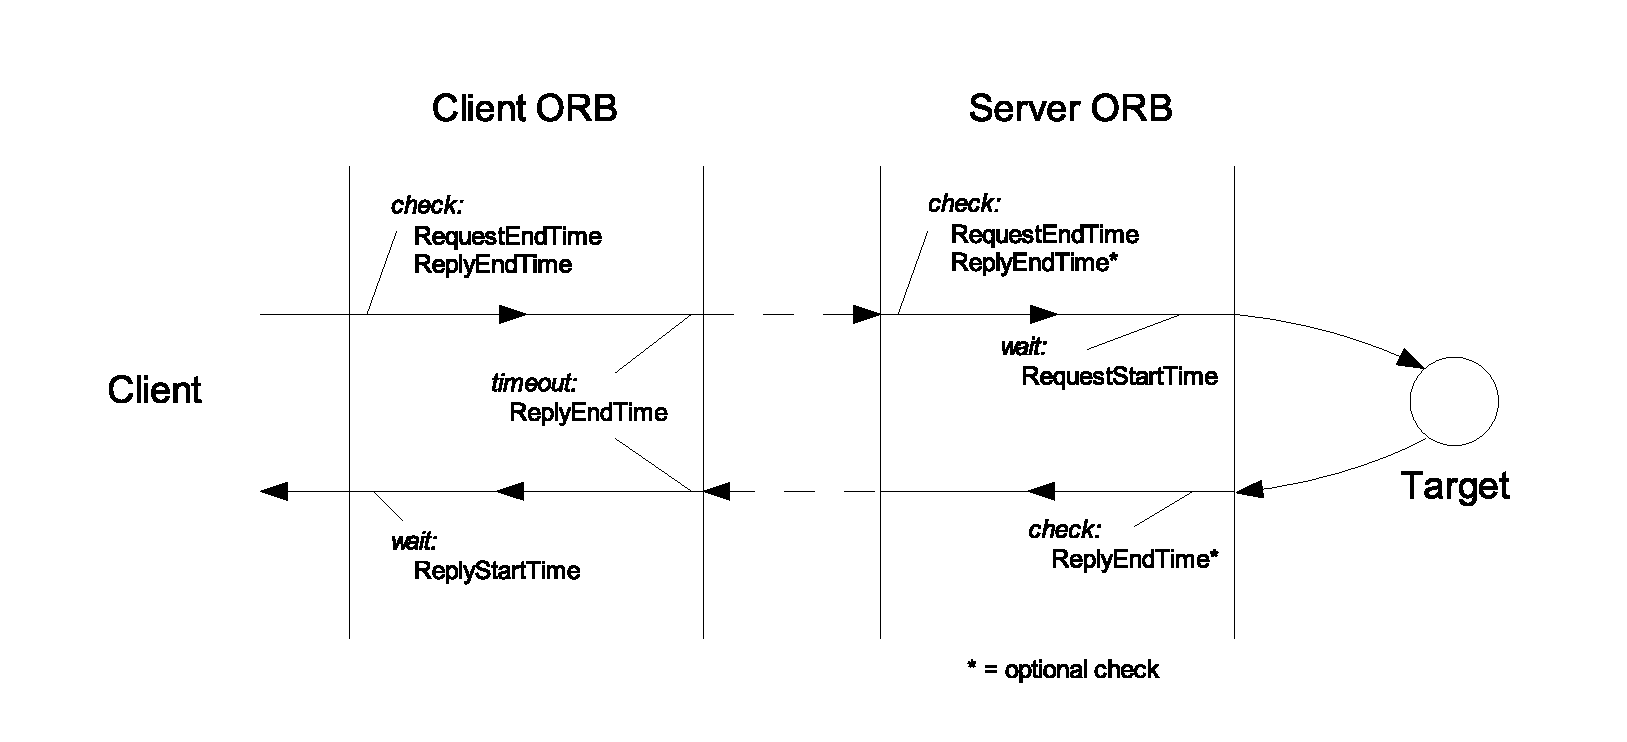
\includegraphics[width=16cm]{QoS/Timing}
  \end{center}
\caption{Timing Policies in JacORB}
\label{fig:timing}
\end{figure}

Figure \ref{fig:timing} shows how JacORB interprets the timing
policies in the course of a single request.

\begin{itemize}
\item As soon as the ORB receives control (prior to marshaling), it
converts any \emph{RelativeRequestTimeoutPolicy} or
\emph{RelativeRoundtripTimeoutPolicy} to an absolute value, by adding
the relative value to the current system time.

\item The ORB then checks whether \emph{Request End Time} or
\emph{Reply End Time} have already elapsed.  If so, no invocation is
made, and an {\tt org.omg.CORBA.TIMEOUT} is thrown to the client.

\item After the ORB has sent the request, it waits for a reply until
\emph{Reply End Time} has elapsed.  If it receives no reply before
that, the request is discarded and an {\tt org.omg.CORBA.TIMEOUT}
thrown to the client.  (JacORB does not currently cancel the
outstanding request, it simply discards the reply, should one arrive
after the timeout has elapsed.)

\item On the server side (before demarshaling), the ORB checks
whether \emph{Request End Time} or \emph{Reply End Time} have already
elapsed.  If so, the request is not delivered to the target, and an
{\tt org.omg.CORBA.TIMEOUT} is thrown back to the client.

\item If the request proceeds, the ORB waits until the \emph{Reply
Start Time} has been reached, if one was specified, and has not
already elapsed.  After that, the request is delivered to the target.

\item After the target has returned control to the ORB, it checks
whether \emph{Reply End Time} has already elapsed.  If it has, the ORB
sends an {\tt org.omg.CORBA.TIMEOUT} back to the client, rather than
the actual reply.

\item If the reply arrives at the client before \emph{Reply End Time}
has elapsed, the ORB waits until \emph{Reply Start Time} has been
reached, if one was specified, and has not already elapsed.  After
that, the reply is delivered back to the client.

\end{itemize}

The bottom line of this is that for a simple, per-invocation timeout,
you should specify a \mbox{\emph{RelativeRoundtripTimeoutPolicy}}.  Note
that since this relative time is converted into an absolute time, and
also checked on the server side, the clocks on both the server and
the client need to be synchronized at least to the same order of
magnitude as the desired timeout.

\subsection*{Programming}

In CORBA, points of time are specified to an accuracy of 100~ns, using
values of struct {\tt TimeBase::UtcT}.  To allow easy manipulation of such
values from Java, JacORB provides a number of static methods in {\tt
org.jacorb.util.Time}.  For example, to convert the current Java time
into a {\tt UtcT} value, write

\begin{verbatim}
UtcT currentTime = org.jacorb.util.corbaTime();
\end{verbatim}

To create a {\tt UtcT} value that specifies a time $n$~ms in the
future, you can write

\begin{verbatim}
UtcT time = org.jacorb.util.corbaFuture (10000 * n);
\end{verbatim}

(The argument to {\tt corbaFuture()} is in CORBA time units of
100~ns; we multiply $n$ by 10000 here to convert it from Java time
units (milliseconds).)

The following shows how to set a timing policy for an object using the
standard mechanism (see the beginning of this chapter for an
explanation).  In this example, we set a \emph{Reply End Time} that
lies one second in the future:

\clearpage{}

\begin{verbatim}
import org.omg.CORBA.*;

SomeCorbaType server  = ...  // the object for which we want to set
                             // a timing policy
org.omg.CORBA.ORB orb = ...
org.omg.CORBA.Any a   = orb.create_any();

org.omg.TimeBase.UtcT replyEndTime
    = org.jacorb.util.Time.corbaFuture (1000);  // one second

org.omg.TimeBase.UtcTHelper.insert (a, replyEndTime);

try
{
    Policy p
        = orb.create_policy (REPLY_END_TIME_POLICY_TYPE.value, a);
    server._set_policy_override (new Policy[]{ p },
                                 SetOverrideType.ADD_OVERRIDE);
}
catch (PolicyError e)
{
    ...
}
\end{verbatim}

Using the constructors of JacORB's implementations of policy values,
this becomes less verbose:

\begin{verbatim}
SomeCorbaType server  = ...

Policy p = new org.jacorb.orb.policies.ReplyEndTimePolicy
                         (org.jacorb.util.Time.corbaFuture (1000));

server._set_policy_override (new Policy[]{ p },
                             SetOverrideType.ADD_OVERRIDE);
\end{verbatim}

Likewise, to set a \emph{Relative Roundtrip Timeout} of one second,
write:

\begin{verbatim}
SomeCorbaType server  = ...

Policy p =
    new org.jacorb.orb.policies.RelativeRoundtripTimeoutPolicy (1000);

server._set_policy_override (new Policy[]{ p },
                             SetOverrideType.ADD_OVERRIDE);
\end{verbatim}

The difference between this and the example before, where a
\emph{Reply End Time} was used, is that the latter specifies a
\emph{relative time} to CORBA.  The policy will therefore be valid
for all subsequent invocations, because the absolute deadline will be
recomputed before each invocation.  In the first example, the
deadline will no longer make sense for any subsequent invocations,
since only an absolute time was specified to the ORB.


%%% Local Variables: 
%%% mode: latex
%%% TeX-master: "../ProgrammingGuide"
%%% End: 


%%%%%%%%%%%%%%%%%%%%%%%%%%%%%%%%%%%%%%%%%%%%%%%%%%%%%%%%%%%%%%%%%%%%%%%%%%%%%%

\chapter{Connection Management and Connection Timeouts}
\label{ch:connections}


JacORB offers a certain level of control over connections and timeouts. You
can
\begin{itemize}
\item set connection idle timeouts.
\item set request timing.
\item set the maximum number of accepted TCP/IP connections on the server.
\end{itemize}

\section{Timeouts}
\label{connection_timeouts}
Connection idle timeouts can be set individually for the client and the
server. They control how long an idle connection, i.e.~a connection that has
no pending replies, will stay open. The corresponding properties are {\tt
  jacorb.connection.client.idle\_timeout} and {\tt
  jacorb.connection.server.timeout} and take their values as milliseconds. If
not set, connections will stay open indefinitely (or until the OS decides to
close them).

\emph{Request timing} controls how long an individual request may take to
complete.  The programmer can specify this using QoS policies,
discussed in chapter \ref{ch:qos}.

\section{Connection Management}
\label{connection_management}

When a client wants to invoke a remote object, it needs to send the request
over a connection to the server. If the connection isn't present, it has to be
created. In JacORB, this will only happen once for every combination of host
name and port. Once the connection is established, all requests and replies
between client and server will use the same connection. This saves resources
while adding a thin layer of necessary synchronization, and is the recommended
approach of the OMG. Occasionally people have requested to allow for multiple
connections to the same server, but nobody has yet presented a good argument
that more connections would speed up things considerably.

On the server side, the property {\tt
  jacorb.connection.max\_server\_connection} allows to set the maximum number
of TCP/IP connections that will be listened on for requests. When using a
network sniffer or tools like netstat, more inbound TCP/IP connections than
the configured number may be displayed. This is for the following reason:
Whenever the connection limit is reached, JacORB tries to close existing idle
connections (see the subsection below). This is done on the thread
that accepts the new connections, so JacORB will not actively accept more
connections. However, the ServerSocket is initialized with a backlog of 20.
This means that 20 more connections will be quasi-accepted by the OS. Only the
21st will be rejected right away.

\subsection{Basics and Design}
\label{connection_management_basics}
Whenever there is the need to close an existing connection because of the
connection limit, the question arises on which of the connection to close. To
allow for maximum flexibility, JacORB provides the interface {\tt
  SelectionStrategy} that allows for a custom way to select a connection to
close. Because selecting a connection usually requires some sort of
statistical data about it, the interface {\tt
  StatisticsProvider} allows to implement a class that collects statistical
data.

\begin{small}
\begin{verbatim}
package org.jacorb.orb.giop;

public interface SelectionStrategy
{
    public ServerGIOPConnection
        selectForClose( java.util.List connections );
}

public interface StatisticsProvider
{
    public void messageChunkSent( int size );
    public void flushed();
    public void messageReceived( int size );
}
\end{verbatim}
\end{small}

The interface {\tt SelectionStrategy} has only the single method of {\tt
  selectForClose()}. This is called by the class {\tt GIOPConnectionManager}
when a connection needs to be closed. The argument is a {\tt List} containing
objects of type {\tt ServerGIOPConnection}. The call itself is synchronized in
the {\tt GIOPConnectionManager}, so no additional synchronization has to be
done by the implementor of {\tt SelectionStrategy}. When examining the
connections, the strategy can get hold of the {\tt StatisticsProvider} via the
method {\tt getStatisticsProvider()} of the class {\tt GIOPConnection}. The
strategy implementor should take care only to return idle connections. While
the connection state is checked anyway while closing (it may have changed in
the meantime), it seems to be more efficient to avoid cycling through the
connections. When no suitable connection is available, the strategy may
return {\tt null}. The {\tt GIOPConnectionManager} will then wait for a
configurable time, and try again. This goes on until a connection can be
closed.

The interface {\tt StatisticsProvider} is used to collect statistical data
about a connection and provide it to the {\tt SelectionStrategy}.  Because the
nature of this data may vary, there is no standard access to the data via the
interface. Therefore, {\tt StatisticsProvider} and {\tt SelectionStrategy}
usually need to be implemented together. Whenever a new connection is
created\footnote{Currently, connection management is only implemented for the
server side. Therefore, only accepted {\tt ServerGIOPConnections}s will get a
{\tt StatisticsProvider}}, a new {\tt StatisticsProvider} object is
instanciated and stored with the {\tt GIOPConnection}\footnote{This is
actually only done when a {\tt StatisticsProvider} is configured}.
The {\tt StatisticsProvider} interface is oriented along the mode of use of the {\tt
GIOPConnection}. For efficiency reasons, messages are not sent as one big byte
array. Instead, they are sent piecewise over the wire. When such a chunk is
sent, the method {\tt messageChunkSent(int size)} will be called. After the
message has been completely sent, method {\tt flush()} is called. This whole
process is synchronized, so all consecutive {\tt messageChunkSent}s until a
{\tt flush()} form a single message. Therefore, no synchronization on this
level is necessary. However, access to gathered statistical data by the {\tt
SelectionStrategy} is concurrent, so care has to be taken. Receiving messages
is done only on the whole, so there exists only one method, {\tt
messageReceived(int size)}, to notify the {\tt StatisticsProvider} of such an
event.


JacORB comes with two pre-implemented strategies: least frequently used and
least recently used. LFU and LRU are implemented by the classes {\tt
  org.jacorb.orb.giop.L[F|R]USelection\-StrategyImpl} and {\tt
  org.jacorb.orb.giop. L[F|R]U\-Statistics\-ProviderImpl}.

\subsection{Configuration}
\label{connection_management_config}
To configure connection management, the following properties are provided:
\begin{description}
\item {\tt jacorb.connection.max\_server\_connections} This property sets the
  maximum number of TCP/IP connections that will be listened on by the
  server--side ORB.
\item {\tt jacorb.connection.wait\_for\_idle\_interval} This property sets the
  interval to wait until the next try is made to find an idle connection to
  close. Value is in microseconds.
\item {\tt jacorb.connection.selection\_strategy\_class} This property sets
  the {\tt Selection\-Strategy}.
\item {\tt jacorb.connection.statistics\_provider\_class} This property sets
  the {\tt Statistics\-Provider}.
\item {\tt jacorb.connection.delay\_close} If turned on, JacORB will delay
  closing of TCP/IP connections to avoid certain situations, where message
  loss can occur. See also section \ref{connection_management_limitations}.
\end{description}

\subsection{Limitations}
\label{connection_management_limitations}
When trying to close a connection, it is first checked that the connection is
idle, i.e.~has no pending messages.  If this is the case, a GIOP
CloseConnection message is sent, and the TCP/IP connection is closed. Under
high load, this can lead to the following situation:

\begin{enumerate}
\item Server sends the CloseConnection message.
\item Server closes the TCP/IP connection.
\item The client sends a new request into the connection, because it hasn't
  yet read and acted on the CloseConnection message.
\item The server--side OS will send a TCP RST, which cancels out the
  CloseConnection message.
\item The client finds the connection closed and must consider the request lost.
\end{enumerate}

To get by this situation, JacORB takes the following approach. Instead
of closing the connection right after sending the CloseConnection
message, we delay closing and wait for the client to close the
connection. This behaviour is turned off by default, but can be
enabled by setting the property {\tt jacorb.connection.delay\_close}
to ``yes''. When non-JacORB clients are used care has to be taken that
these ORBs do actively close the connection upon receiving a
CloseConnection message.


%%% Local Variables:
%%% mode: latex
%%% TeX-master: "../ProgrammingGuide"
%%% End:


%%%%%%%%%%%%%%%%%%%%%%%%%%%%%%%%%%%%%%%%%%%%%%%%%%%%%%%%%%%%%%%%%%%%%%%%%%%%%%

\chapter{Extensible Transport Framework}
\label{ch:etf}


The \emph{Extensible Transport Framework (ETF)}, which JacORB
implements, allows you to plug in other transport layers besides the
 standard IIOP (TCP/IP) protocol\footnote{At the time of
 this writing (July 2003), ETF is still a draft standard (OMG TC
 document mars/2003-02-01).}.

To use an alternative transport, you need to (a) implement it as a set
of Java classes following the ETF specification, and (b) tell JacORB
to use the new transport instead of (or alongside with) the standard
IIOP transport.  We cover both steps below.

\section{Implementing a new Transport}

The interfaces that an ETF-compliant transport must implement are
 described in the ETF specification, and there is thus no need to
 repeat that information here.  JacORB's default IIOP transport, which
 is realized in the package {\tt org.jacorb.orb.iiop}, can also serve
 as a starting point for implementing your own transports.

For each transport, the following interfaces must be implemented
(defined in {\tt ETF.idl}, the package is {\tt org.omg.ETF}):

\begin{description}
\item[Profile] encapsulates addressing information for this transport
\item[Listener] server-side communication endpoint, waits for incoming
connections and passes them up to the ORB
\item[Connection] an actual communication channel for this transport
\item[Factories] contains factory methods for the above interfaces
\end{description}

The {\tt Handle} interface from the ETF package is implemented in the
 ORB (by the class {\tt org.jacorb.orb.BasicAdapter}), not by
 individual transports.  There is currently no support in JacORB for
 the optional zero-copy mechanism; the interface {\tt
 ConnectionZeroCopy} therefore needn't be implemented.

On the server side, the {\tt Listener} must pass incoming connections
 up to the ORB using the ``Handle'' mechanism; the {\tt accept()}
 method needn't be implemented.  Once a {\tt Connection} has been
 passed up to the ORB, it will never be ``returned'' to the {\tt
 Listener} again.  The method {\tt completed\_data()} in the {\tt
 Listener} interface therefore needn't be implemented, and neither
 should the {\tt Listener} ever call {\tt
 Handle.signal\_data\_available()} or {\tt Handle.closed\_by\_peer()}
 (these methods throw a {\tt NO\_IMPLEMENT} exception in JacORB).

At the time of this writing (July 2003), there is still uncertainty in
 ETF about how server-specific Profiles (as returned by {\tt
 Listener.endpoint()}, for example) should be turned into
 object-specific ones for inclusion into IORs.  We have currently
 added three new operations to the {\tt Profile} interface to resolve
 this issue, see JacORB's version of {\tt ETF.idl} for details.

\section{Configuring Transport Usage}

You tell JacORB which transports it should use by listing the names of
 their {\tt Factories} classes in the property {\tt
 jacorb.transport.factories}.  In the standard configuration, this
 property contains only {\tt org.jacorb.orb.iiop.IIOPFactories}, the
 {\tt Factories} class for the standard IIOP transport.  The
 property's value is a comma-separated list of fully qualified Java
 class names; each of these classes must be found somewhere on the
 CLASSPATH that JacORB is started with.  For example:

\begin{scriptsize}
\begin{verbatim}
jacorb.transport.factories = my.transport.Factories, org.jacorb.orb.iiop.IIOPFactories
\end{verbatim}
\end{scriptsize}

By default, a JacORB server creates listeners for each transport
listed in the above property, and publishes profiles for each of these
transports in any IOR it creates.  The order of profiles within an IOR
is the same as that of the transports in the property.

If you don't want your servers to listen on each of these transports
 (e.g. because you want some of your transports only to be used for
 client-side connections), you can specify the set of actual listeners
 in the property {\tt jacorb.transport.server.listeners}.  The value
 of this property is a comma-separated list of numeric profile tags,
 one for each transport that you want listeners for, and which you
 want published in IOR profiles.  The numeric value of a transport's
 profile tag is the value returned by the implementation of {\tt
 Factories.profile\_tag()} for that transport.  Standard IIOP has
 profile tag 0 ({\tt TAG\_INTERNET\_IOP}).  Naturally, you can only
 specify profile tag numbers here for which you have a corresponding
 entry in {\tt jacorb.transport.factories}.

So, to restrict your server-side transports to standard IIOP, you
would write:

\begin{verbatim}
jacorb.transport.server.listeners = 0
\end{verbatim}

On the client side, the ORB must decide which of potentially many
 transports it should use to contact a given server.  The default
 strategy is that for each IOR, the client selects \emph{the first profile
 for which there is a transport implementation available at the client
 side} (specified in {\tt jacorb.transport.factories}).  Profiles for
which the client has no transport implementation are skipped.

Note that this is a purely static decision, based on availability of
 an implementation.  JacORB does not attempt to actually establish a
 transport connection in order to find out which transport can be
 used.  Also, should the selected transport fail, JacORB does not
 ``fall back'' to the next transport in the list.  (This is because
 JacORB opens connections lazily, only when the first actual data is
 being sent.)

You can customize this strategy by providing your own implementation of
{\tt org.jacorb.orb.ProfileSelector}, and specifying it in the
property {\tt jacorb.transport.client.selector}.  The interface {\tt
ProfileSelector} requires a single method,

\begin{verbatim}
   public Profile selectProfile (List profiles,
                                 ClientConnectionManager ccm);
\end{verbatim}

For each IOR, this method receives a list of all profiles from the IOR
 for which the client has a transport implementation, in the order in
 which they appear in the IOR.  The method should select one profile
 from this list and return it; this profile will then be used for
 communication with the server.

To help with the decision, JacORB's {\tt ClientConnectionManager} is
 passed as an additional parameter.  The method implementation can use
 it to check whether connections with a given transport, or to a given
 server, have already been made; it can also try and pre-establish a
 connection using a given transport and store it in the {\tt
 ClientConnectionManager} for later use.  (See the JacORB source code
to find out how to deal with the {\tt ClientConnectionManager}.)

The default {\tt ProfileSelector} does not use the {\tt
 ClientConnectionManager}, it simply returns the first profile from
 the list, unconditionally.  To let JacORB use your own implementation
 of the {\tt ProfileSelector} interface, specify the fully qualified
 classname in the property:

\begin{verbatim}
jacorb.transport.client.selector=my.pkg.MyProfileSelector
\end{verbatim}


%%% Local Variables: 
%%% mode: latex
%%% TeX-master: "../ProgrammingGuide"
%%% End: 


%%%%%%%%%%%%%%%%%%%%%%%%%%%%%%%%%%%%%%%%%%%%%%%%%%%%%%%%%%%%%%%%%%%%%%%%%%%%%%

\chapter{JacORB utilities}
\label{ch:tools}

%
% $Id: tools.tex,v 1.14 2009-11-27 14:53:14 alexander.bykov Exp $
%

In this chapter we  briefly explain the executables that come
with JacORB. These include the IDL-compiler, a utility to decode IORs
and print their components, the JacORB name server, a utility to test
a remote object's liveness, etc.

\section{idl}

The IDL compiler parses IDL files and maps type definitions to Java
classes as specified by the OMG IDL/Java language mapping. For
example, IDL interfaces are translated into Java interfaces, and
typedefs, structs, const declarations etc.  are mapped onto
corresponding Java classes. Additionally, stubs and skeletons for all
interface types in the IDL specification are generated.

(The  IDL  parser  was   generated  with  Scott  Hudson's  CUP  parser
generator.  The  LALR grammar for  the CORBA IDL  is in the  file {\tt
org/jacorb/idl/parser.cup}.)

\subsection*{Compiler Options}

\begin{tabbing}
XX \= XXXXXXXXXXXXX \= XX \kill
\>  -h $|$ help \>  print help on compiler options\\
\>  -v $|$ version \> print compiler version information\\
\>  -d dir \> root of directory tree for output (default: current directory)\\
\>  -syntax \> syntax check only, no code generation\\
\>  -Dx \>  define preprocessor symbol x with value 1\\
\>  -Dx=y  \>  define preprocessor symbol x with value y\\
\>  -Idir  \>  set include path for idl files\\
\>  -Usymbol \> undefine preprocessor symbol\\
\>  -W [1..4] \> debug output level (default is 1)\\
\>  -all  \> generate code for all IDL files, even included ones
(default is off)\\
\> \> If you want to make sure that for a given IDL no code will\\
\> \>  be generated even if this option is set, use the (proprietary)
preprocessor \\
\> \> directive {\tt \#pragma   inhibit\_code\_generation}.\\
\>  -forceOverwrite \> generate Java code even if the IDL files have
not \\
\> \> changed since the last compiler run (default is off)\\
\>  -ami\_callback  \> generate AMI reply handlers and sendc methods
(default is off). See chapter \ref{ch:AMI}\\
\>  -ami\_polling  \>  generate AMI poller and sendp methods (default
is off). See chapter \ref{ch:AMI}\\
\>  -addbackend classname \>  classname as code generator\\
\>  -backend classname \>  use classname as compiler (code generator) backend.\\
\> \>If no generator is specified then it will default to simple file output.\\
\> \>Custom generators must implement the interface\\
\> \> {\tt org.jacorb.idl.IDLTreeVisitor}\\
\> -i2jpackage x:a.b.c \>  replace IDL package name x by a.b.c in
generated Java code \\
\> \> (e.g. CORBA:org.omg.CORBA)\\
\> -i2jpackagefile filename \> replace IDL package names using list
from <filename>. \\
\> \> Format as above.\\
\> -ir \> generate extra information required by the JacORB Interface
Repository \\
\> \> (One extra file for each IDL module, and another additional file per IDL interface.)\\
\> \> (default is off)\\
\> -cldc10 \>Generate J2ME/CLDC1.0 compliant stubs\\
\> -genEnhanced \>Generate stubs with toString/equals (only StructType)\\
\> -nofinal  \> generated Java code will contain no final class
definitions, which\\
\> \> is the default to allow for compiler optimizations.\\
\> -unchecked\_narrow  \>  use unchecked\_narrow in generated code for IOR parameters in
 operations \\
\> \> (default is off). Generated helper classes contain marshalling code which, by
default,\\
\> \>  will try to narrow any object references to statically known interface type. This \\
\> \> may involve remote invocations to test a remote object's type, thus incurring \\
\> \> runtime overhead to achieve static type safety. The -unchecked\_narrow option\\
\> \> generates code that will not by statically type safe, but avoids
remote tests \\
\> \>  of an object's type. If the type is not as expected, clients will experience \\
\> \> CORBA.BAD\_OPERATION exceptions at invocation time.\\
\> -noskel \>disables generation of POA skeletons (e.g., for
client-side use)\\
\> -nostub \>disables generation of client stubs (for server-side use)\\
\> -diistub \>generate DII-based client stubs \\
\> \> (default is off)\\
\> -sloppy\_forward \> allow forward declarations without later
definitions\\
\> \> (useful only for separate compilation).\\
\> -sloppy\_names \> less strict checking of module name scoping
(default: off)\\
\> \> CORBA IDL has a number of  name resolution rules that are
stricter than\\
\> \> necessary for Java (e.g., a struct member's name identifier must
not \\
\> \> equal the type name). The -sloppy\_names option relaxes checking of
these \\
\> \>  rules. Note that IDL accepted with this option will be rejected
by other, conformant  \\
\> \> IDL compilers!\\
\> -permissive\_rmic  \>  tolerate dubious and buggy IDL generated by
JDK's rmic stub generator\\
\> \> (e.g., incorrectly empty inheritance clauses), includes -sloppy\_names.\\
\> -generate\_helper \emph{compatibilty} \\
\> \> controls the compatibilty level of the generated helper code. Valid values are: \\
\> \> {\bf deprecated} uses CORBA 2.3 API. this API version is part of the JDK.\\
\> \> {\bf portable} uses CORBA 2.4 API. the usage of this option mandates the use \\
\> \> of the JacORB provided \emph{org.omg.*} classes on the bootclasspath. This is the default. \\
\> \> {\bf jacorb} uses JacORB API. The generated helper code will contain references \\
\> \> to JacORB classes. The helpers will use the CORBA 2.4 API but won't be portable \\
\> \> anymore. There's no need to put the \emph{org.omg.*} classes provided by JacORB \\
\> \> on the bootclasspath.
\end{tabbing}

\subsection*{i2jpackage}
The {\tt -i2jpackage} switch can be used to flexibly redirect
generated Java classes into packages. Using this option, any IDL scope
x can be replaced by one (or more) Java packages y. Specifying {\tt
  -i2jpackage X:a.b.c} will thus cause code generated for IDL
definitions within a scope x to end up in a Java package {\tt a.b.c},
e.g. an IDL identifier {\tt X::Y::ident} will be mapped to {\tt
  a.b.c.y.ident} in Java. It is also possible to specify a file
containing these mappings using the {\tt -i2jpackagefile} switch.

\subsubsection{Example 1}

given the following IDL definition
\begin{verbatim}
struct MyStruct
{
    long value;
};
\end{verbatim}
Invoking idl without the i2jpackage option will generate (along with other
files) the java file MyStruct.java
\begin{verbatim}

/**
 * Generated from IDL struct "MyStruct".
 *
 * @author JacORB IDL compiler V 2.3, 18-Aug-2006
 * @version generated at 07.12.2006 11:46:28
 */

public final class MyStruct
        implements org.omg.CORBA.portable.IDLEntity
{
    [...]
}
\end{verbatim}

Note that the class does not contain a package definition.

The option -i2jpackage :com.acme will place any identifier without scope into
the java package com.acme. Thus we get:
\begin{verbatim}
package com.acme;

/**
 * Generated from IDL struct "MyStruct".
 *
 * @author JacORB IDL compiler V 2.3, 18-Aug-2006
 * @version generated at 07.12.2006 11:46:28
 */

public final class MyStruct
        implements org.omg.CORBA.portable.IDLEntity
{
    [...]
}
\end{verbatim}

\subsubsection{Example 2}

\begin{verbatim}
module outer
{
    struct OuterStruct
    {
        long value;
    };

    module inner
    {
        struct InnerStruct
        {
            long value;
        };
    };
};
\end{verbatim}

If you're not using the i2jpackage option, the IDL compiler will generate
the classes \emph{outer.OuterStruct} and \emph{outer.inner.InnerStruct}.

Again using the i2jpackage it's possible to map IDL modules to different java
packages.
\cmdline{idl -i2jpackage outer:com.acme.outer} will generate the classes
\emph{com.acme.outer.OuterStruct} and \emph{com.acme.outer.inner.InnerStruct}.

\cmdline{idl -idjpackage inner:com.acme.inner} will generate the classes
\emph{outer.OuterStruct} and \emph{outer.com.acme.inner.InnerStruct}.

Note: See Section \ref{sec:ifr_pragma_i2jpackage} if you intend to use the
i2jpackage option in conjunction with the JacORB IfR and are using \#pragma
prefix statements in your IDL.


\subsection*{Compiler Options}
If one is building from Ant it is possible to invoke the compiler directly
using the supplied Ant task, JacIDL. To add the taskdef add the following
to the ant script:
\small{
\begin{verbatim}
<taskdef name="jacidl" classname="org.jacorb.idl.JacIDL"/>
\end{verbatim}
}
The task supports all of the options of the IDL compiler.

\begin{small}
\begin{longtable}{|p{4cm}|p{8.5cm}|p{2cm}|p{2cm}|}
\caption{JacIDL Configuration}\\
\hline
~ \hfill \textbf {Attribute} \hfill ~ & ~ \hfill \textbf {Description} \hfill ~ & ~ \hfill \textbf{Required} \hfill ~ & ~ \hfill \textbf {Default} \hfill ~ \endhead
\hline
\verb"srcdir" & Location of the IDL files & Yes & \\
\hline
\verb"destdir" & Location of the generated java files & Yes & \\
\hline
\verb"includes" & Comma-separated list of patterns of files that must be included; all files are included when omitted. & No & \\
\hline
\verb"includesfile" & The name of a file that contains include patterns. & No & \\
\hline
\verb"excludes" & Comma-separated list of patterns of files that must be excluded; files are excluded when omitted. & No & \\
\hline
\verb"excludesfile" & The name of a file that contains include patterns. & No & \\
\hline
\verb"defaultexcludes" & Indicates whether default excludes should be used (yes | no); default
excludes are used when omitted. & No & \\
\hline
\verb"includepath" & The path the idl compiler will use to search for included files. & No & \\
\hline
\verb"parseonly" & Only perform syntax check without generating code. & No & False\\
\hline
\verb"noskel" & Disables generation of POA skeletons & No & False\\
\hline
\verb"nostub" & Disables generation of client stubs & No & False\\
\hline
\verb"diistub" & Generate DII-based client stubs & No & False\\
\hline
\verb"sloppyforward" & Allow forward declarations without later definitions & No & False\\
\hline
\verb"sloppynames" & Less strict checking of names for backward compatibility & No & False\\
\hline
\verb"generateir" & Generate information required by the Interface Repository & No & False\\
\hline
\verb"all" & Generate code for all IDL files, even included ones & No & False\\
\hline
\verb"nofinal" & Generate class definitions that are not final & No & False\\
\hline
\verb"forceoverwrite" & Generate code even if IDL has not changed. & No & False\\
\hline
\verb"uncheckedNarrow" & Use unchecked\_narrow in generated code for IOR parameters in operations. & No & False\\
\hline
\verb"ami" & Generate ami callbacks. & No & False\\
\hline
\verb"debuglevel" & Set the debug level from 0 to 4. & No & 0\\
\hline
\verb"helpercompat" & control the portability of the generated helper code. & No & portable \\
\hline
\end{longtable}
\end{small}

\subsection*{Nested Elements}

Several elements may be specified as nested elements. These are {\tt <define>}, {\tt <undefine>}, {\tt <include>}, {\tt <exclude>}, {\tt <patternset>} and {\tt <i2jpackage>}. The format of {\tt <i2jpackage>} is {\tt <i2jpackage names="x:y">}


\subsection*{Examples}

The task command
\small{\begin{verbatim}
    <jacidl destdir="${generate}"
            srcdir="${idl}"
    />
\end{verbatim}
}

compiles all *.idl files under the \${idl} directory and stores the .java files in the \${generate} directory.

\small{\begin{verbatim}
    <jacidl destdir="${generate}" srcdir="${idl}">
       <define key="GIOP_1_1" value="1"/>
    </jacidl>
\end{verbatim}
}

like above, but additionaly defines the symbol GIOP\_1\_1 and sets its (optional) value to 1.

\small{\begin{verbatim}
    <jacidl destdir="${generate}"
            srcdir="${idl}"
            excludes="**/*foo.idl"
    />
\end{verbatim}
}

like the first example, but exclude all files which end with foo.idl.

\section{ns}

JacORB provides a service for mapping names to network references. The
name server itself is written in Java like the rest of the package and
is a  straightforward implementation  of the CORBA  ``Naming Service''
from  Common  Object Services  Spec.,  Vol.1  \cite{OMG1997}. The  IDL
interfaces are mapped to Java according to our Java mapping.

\subsection*{Usage}

\cmdline{ns <filename>  [<timeout>]}

or

\cmdline{jaco jacorb.Naming.NameServer <filename>  [<timeout>]}

\subsection*{Example}

\cmdline{ns \~/public\_html/NS\_Ref}

The name server does {\it not}  use a well known port for its service.
Since clients  cannot (and  need not) know  in advance where  the name
service will  be provided, we use  a bootstrap file in  which the name
server records  an object reference to itself  (its {\it Interoperable
Object Reference} or  IOR). The name of this bootstrap  file has to be
given as an argument to the  {\tt ns} command. This bootstrap file has
to  be available  to clients  network-wide, so  we demand  that  it be
reachable  via a  URL  --- that  is,  there must  be an  appropriately
configured HTTP server in your network domain which allows read access
to the bootstrap  file over a HTTP connection.  (This implies that the
file must have its read  permissions set appropriately. If the binding
to the name service fails, please  check that this is the case.) After
locating the name service through this mechanism, clients will connect
to the name server directly, so the only HTTP overhead is in the first
lookup of the server.

The name bindings in the server's database are stored in and retrieved
from a file that is found in the current directory unless the property
{\tt jacorb.naming.db\_dir} is set to a different directory name. When
the server  starts up, it tries  to read this file's  contents. If the
file  is  empty or  corrupt,  it will  be  ignored  (but overridden  on
exit). The name server can only save its state when it goes down after
a specified timeout. If the server is interrupted (with {\tt CTRL-C}),
state information  is lost  and the file  will not contain  any usable
data.

If no timeout is specified, the name server will simply stay up until
it is killed. Timeouts are specified in milliseconds.

\section{nmg}

The JacORB  NameManager, a  GUI for the  name service, can  be started
using the {\tt nmg} command.  The NameManager then tries to connect to
an existing name service.

\subsection*{Usage}

\cmdline{nmg}

\section{lsns}

This utility  lists the contents  of the default naming  context. Only
currently active servers that have registered are listed. The {\tt -r}
option recursively lists the  contents of naming contexts contained in
the root  context. If  the graph of  naming contexts  contains cycles,
trying to list the entire contents recursively will not return...

\subsection*{Usage}


\cmdline{lsns [-r] }

\subsection*{Example}

\cmdline{lsns \\
\ /grid.service}

when only the server for the grid example is running and registered
with the name server.


\section{dior}

JacORB comes with a simple utility to decode an interoperable object reference
(IOR) in string form into a more readable representation.

\subsection*{Usage}

\cmdline{dior -i <IOR-string> | -f <filename>}

\subsection*{Example}

In the following example we use it to print out the contents of the
IOR that the JacORB name server writes to its file:

\cmdline{dior -f \~/public\_html/NS\_Ref}
\small{\begin{verbatim}
------IOR components-----
TypeId  :       IDL:omg.org/CosNaming/NamingContextExt:1.0
Profile Id   :  TAG_INTERNET_IOP
IIOP Version :  1.0
Host    :       160.45.110.41
Port    :       49435
Object key :    0x52 6F 6F 74 50 4F 41 3A 3A 30 D7 D1 91 E1 70 95 04
\end{verbatim}
}

\section{pingo}

``Ping'' an object using its stringified IOR. Pingo will call {\tt
  \_non\_existent()} on the object's reference to determine whether
  the object is alive or not.

\subsection*{Usage}

\cmdline{pingo -i <IOR-string> | -f <filename> }

\section{ir}

This command starts the JacORB Interface Repository, which is explained in
chapter \ref{ch:interface_repository}.

\subsection*{Usage}

\cmdline{ir <reppository class path> <IOR filename> }

\section{qir}

This command queries the JacORB Interface Repository and prints out
re--generated IDL for the repository item denoted by the argument
repository ID.

\subsection*{Usage}

\cmdline{qir <reppository Id> }

\section{ks}

This command starts the JacORB KeyStoreManager, which is explained in
chapter \ref{ch:SSL}

\subsection*{Usage}

\cmdline{ks}

\section{fixior}

This command patches host and port information into an IOR file.

\subsection*{Usage}

\cmdline{fixior <host> <port> <ior\_file> }


%%% Local Variables:
%%% mode: latex
%%% TeX-master: "../ProgrammingGuide"
%%% End:



%%%%%%%%%%%%%%%%%%%%%%%%%%%%%%%%%%%%%%%%%%%%%%%%%%%%%%%%%%%%%%%%%%%%%%%%%%%%%%


%%%%%%%%%%%%%%%%%%%%%%%%%%%%%%%%%%%
{
\bibliography{./guide}
\bibliographystyle{alpha}
}

\end{document}
